\documentclass[12pt]{article}

\usepackage{amsmath, amssymb, amsthm}
\usepackage{scalerel,stackengine}
\usepackage{esint}
\usepackage{geometry}
\geometry{a4paper, margin=1in}
\usepackage{setspace}
\doublespacing
\usepackage{titlesec}
\usepackage[autostyle=true]{csquotes}
\usepackage{graphicx}
\usepackage{stmaryrd}
\usepackage{tikz}
\usetikzlibrary{arrows.meta}
\usepackage{fancyhdr}
\usepackage{dsfont}
\usepackage{imakeidx}
\usepackage{microtype}
\usepackage[svgnames]{xcolor}

\usepackage{hyperref}
\hypersetup{
    colorlinks=true,
    linkcolor=NavyBlue,
    citecolor=DarkRed,
    urlcolor=Teal,
}

\usepackage[type={CC}, modifier={by-nc-sa}, version={4.0}]{doclicense}

\usepackage{enumitem}
\setlist{nosep}

\titleformat{\section}
{\normalfont\bfseries\LARGE}
{\thesection}{1em}{}
\titleformat{\subsection}
{\normalfont\bfseries\Large}
{\thesubsection}{1em}{}
\titleformat{\subsubsection}
{\normalfont\itshape\bfseries\large}
{\thesubsubsection}{1em}{}

\newtheoremstyle{blueplain}
  {3pt}{3pt}
  {\itshape}
  {}
  {\color{NavyBlue}\bfseries}
  {.}
  {0.5em}
  {}

\newtheoremstyle{bluedef}
  {3pt}{3pt}
  {\normalfont}
  {}
  {\color{Teal}\bfseries}
  {.}
  {0.5em}
  {}

\newtheoremstyle{blueremark}
  {3pt}{3pt}
  {\normalfont}
  {}
  {\color{DarkRed}\itshape}
  {.}
  {0.5em}
  {}

\theoremstyle{blueplain}
\newtheorem{theorem}{THEOREM}[section]
\newtheorem{proposition}[theorem]{Proposition}
\newtheorem{corollary}[theorem]{Corollary}
\newtheorem{lemma}[theorem]{Lemma}

\theoremstyle{bluedef}
\newtheorem{definition}{DEFINITION}[section]

\theoremstyle{blueremark}
\newtheorem{remark}{Remark}[section]
\newtheorem{example}{Example}[section]


\newcommand{\R}{\mathbb{R}}
\newcommand{\N}{\mathbb{N}}
\newcommand{\C}{\mathbb{C}}
\newcommand{\Z}{\mathbb{Z}}
\newcommand{\Q}{\mathbb{Q}}
\newcommand{\eps}{\varepsilon}
\newcommand{\ups}{\upsilon}
\newcommand{\mL}{\mathcal{L}}

\newcommand{\optsubsection}[1]{%
  \begingroup
    \let\oldthesubsection\thesubsection
    \renewcommand{\thesubsection}{\oldthesubsection$^*$}
    \subsection{#1}%
  \endgroup
}

\numberwithin{equation}{section}

\makeindex[columns=2, title=Index, intoc]

\pagestyle{fancy}
\fancyhf{}
\fancyhead[L]{\textsc{\small Real Analysis}}
\fancyhead[R]{\small \nouppercase{\leftmark}}
\fancyfoot[R]{\hyperref[mytoc]{\Large $\hookleftarrow$}}
\fancyfoot[C]{\thepage}
\fancyfoot[L]{\href{https://creativecommons.org/licenses/by-nc-sa/4.0/deed.en}{\doclicenseIcon}}
\setlength{\headheight}{14pt}
\setlength{\headsep}{20pt}
\setlength{\footskip}{25pt}

\begin{document}

\pagenumbering{gobble}

\begin{titlepage}
  \centering
  \vspace*{3cm}

  {\Huge \bfseries Real Analysis \par}

  \vspace{4cm}

  {\Large Kai Chen \par}
  \vspace{0.5cm}
  {\large \today \par}

  \vfill

  \rule{0.8\textwidth}{0.4pt} \\
  \vspace{0.5cm}
  {\small Part of the \href{https://github.com/kaiiiichen/SUSTech-Kai-Notes/wiki}{SUSTech-Kai-Notes} Initiative}
\end{titlepage}

\newpage
\thispagestyle{empty}

\vspace*{\fill}

\begin{center}
  \copyright\ \the\year\ Kai Chen. All rights reserved.

  \vspace{0.5cm}

  \doclicenseThis

  \vspace{1cm}

  This document was typeset using \href{https://www.latex-project.org}{\LaTeX}.
\end{center}
\clearpage

\pagenumbering{roman}

\section*{Preface}
These notes are compatible with the \href{https://github.com/kaiiiichen/SUSTech-Kai-Notes/tree/main/MA337%20Real%20Analysis%20(H)}{MA337 course (Fall 2025)} at \href{https://www.sustech.edu.cn/}{SUSTech}, and part of the course-notes-and-resources initiative: \href{https://github.com/kaiiiichen/SUSTech-Kai-Notes/wiki}{SUSTech-Kai-Notes}.

\medskip

\noindent I tried my best to make sure every statement and proof correct, and I made some complements, which might be useful, to the original contents of the course. For instance, the Dynkin classes.

\medskip

\vspace{2em}
\noindent\textbf{Main reference:}

\noindent A.N. Kolmogorov and S.V. Fomin, \textit{Elements of the Theory of Functions and Functional Analysis}: translated from the first (1954) Russian edition by Leo F. Boron, Gra Ylock Press, 1957.

\noindent (There is also a Chinese version of the book published by Higher Education Press, 2006.)

\clearpage

\phantomsection

\label{mytoc}

\onehalfspacing

\tableofcontents

\clearpage

\doublespacing

\pagenumbering{arabic}

\section{Set Theory}

This section is a crash course on set theory.

\clearpage

\subsection{Elements of Set Theory}

A set is a collection of well-defined objects. In fact, we cannot have a definable notion of a set.

\underline{Notation}: A set consists of its elements: $a \in A$;

$\emptyset$: empty set, i.e. $\forall x$, it holds $x \notin \emptyset$.

\begin{definition}
  $A \subset B$ ($A$ is \textbf{included in} $B$) if $\forall a \in A \Rightarrow a \in B$.
\end{definition}

\begin{proposition}
  $\forall$ set $A$, $\emptyset \subset A$.
\end{proposition}

\begin{definition}[Complement of a Set]\index{Complement of a Set}

  Let $A \subset \Omega$, then the \textbf{complement} of $A$ in $\Omega$ is defined as $A^c = \{x \in \Omega: x \notin A\}$.
\end{definition}


\underline{Question}: Why should we be careful with the notion of sets?

\begin{example}[Barber's Paradox]\index{Barber's Paradox}

  This is a paradox proposed by British philosopher and mathematician Bertrand Russell.

  Imagine that in a city X, there are residents with one of them being a barber. It's known that the barber only shaves everyone who doesn't shave himself. Does the barber shave himself? This leads to a contradiction.

  Mathematically speaking, there doesn't exist a set of all sets.
\end{example}

\begin{definition}[Power Set]\index{Power Set}


  Let $A$ be a set, then the \textbf{power set} of $A$ is defined as $2^A = \{$ all subsets of $A$ $\}$.
\end{definition}

\begin{proposition}
  $|2^A| = 2^{|A|}$ if $A$ is finite.
\end{proposition}

\begin{definition}[Set Operation]\index{Set Operation}

  Let $A, B$ be two sets, then
  \begin{enumerate}
    \item \textbf{Union}: $A \cup B = \{x: x \in A \text{ or } x \in B\}$.
    \item \textbf{Intersection}: $A \cap B = \{x: x \in A \text{ and } x \in B\}$.
    \item \textbf{Difference}: $A \setminus B = \{x: x \in A \text{ and } x \notin B\}$.
    \item \textbf{Symmetric Difference}: $A \triangle B = (A \setminus B) \cup (B \setminus A)$.
  \end{enumerate}
\end{definition}

\begin{figure}[htbp]
  \centering
  \begin{minipage}[t]{0.4\textwidth}
    \centering
    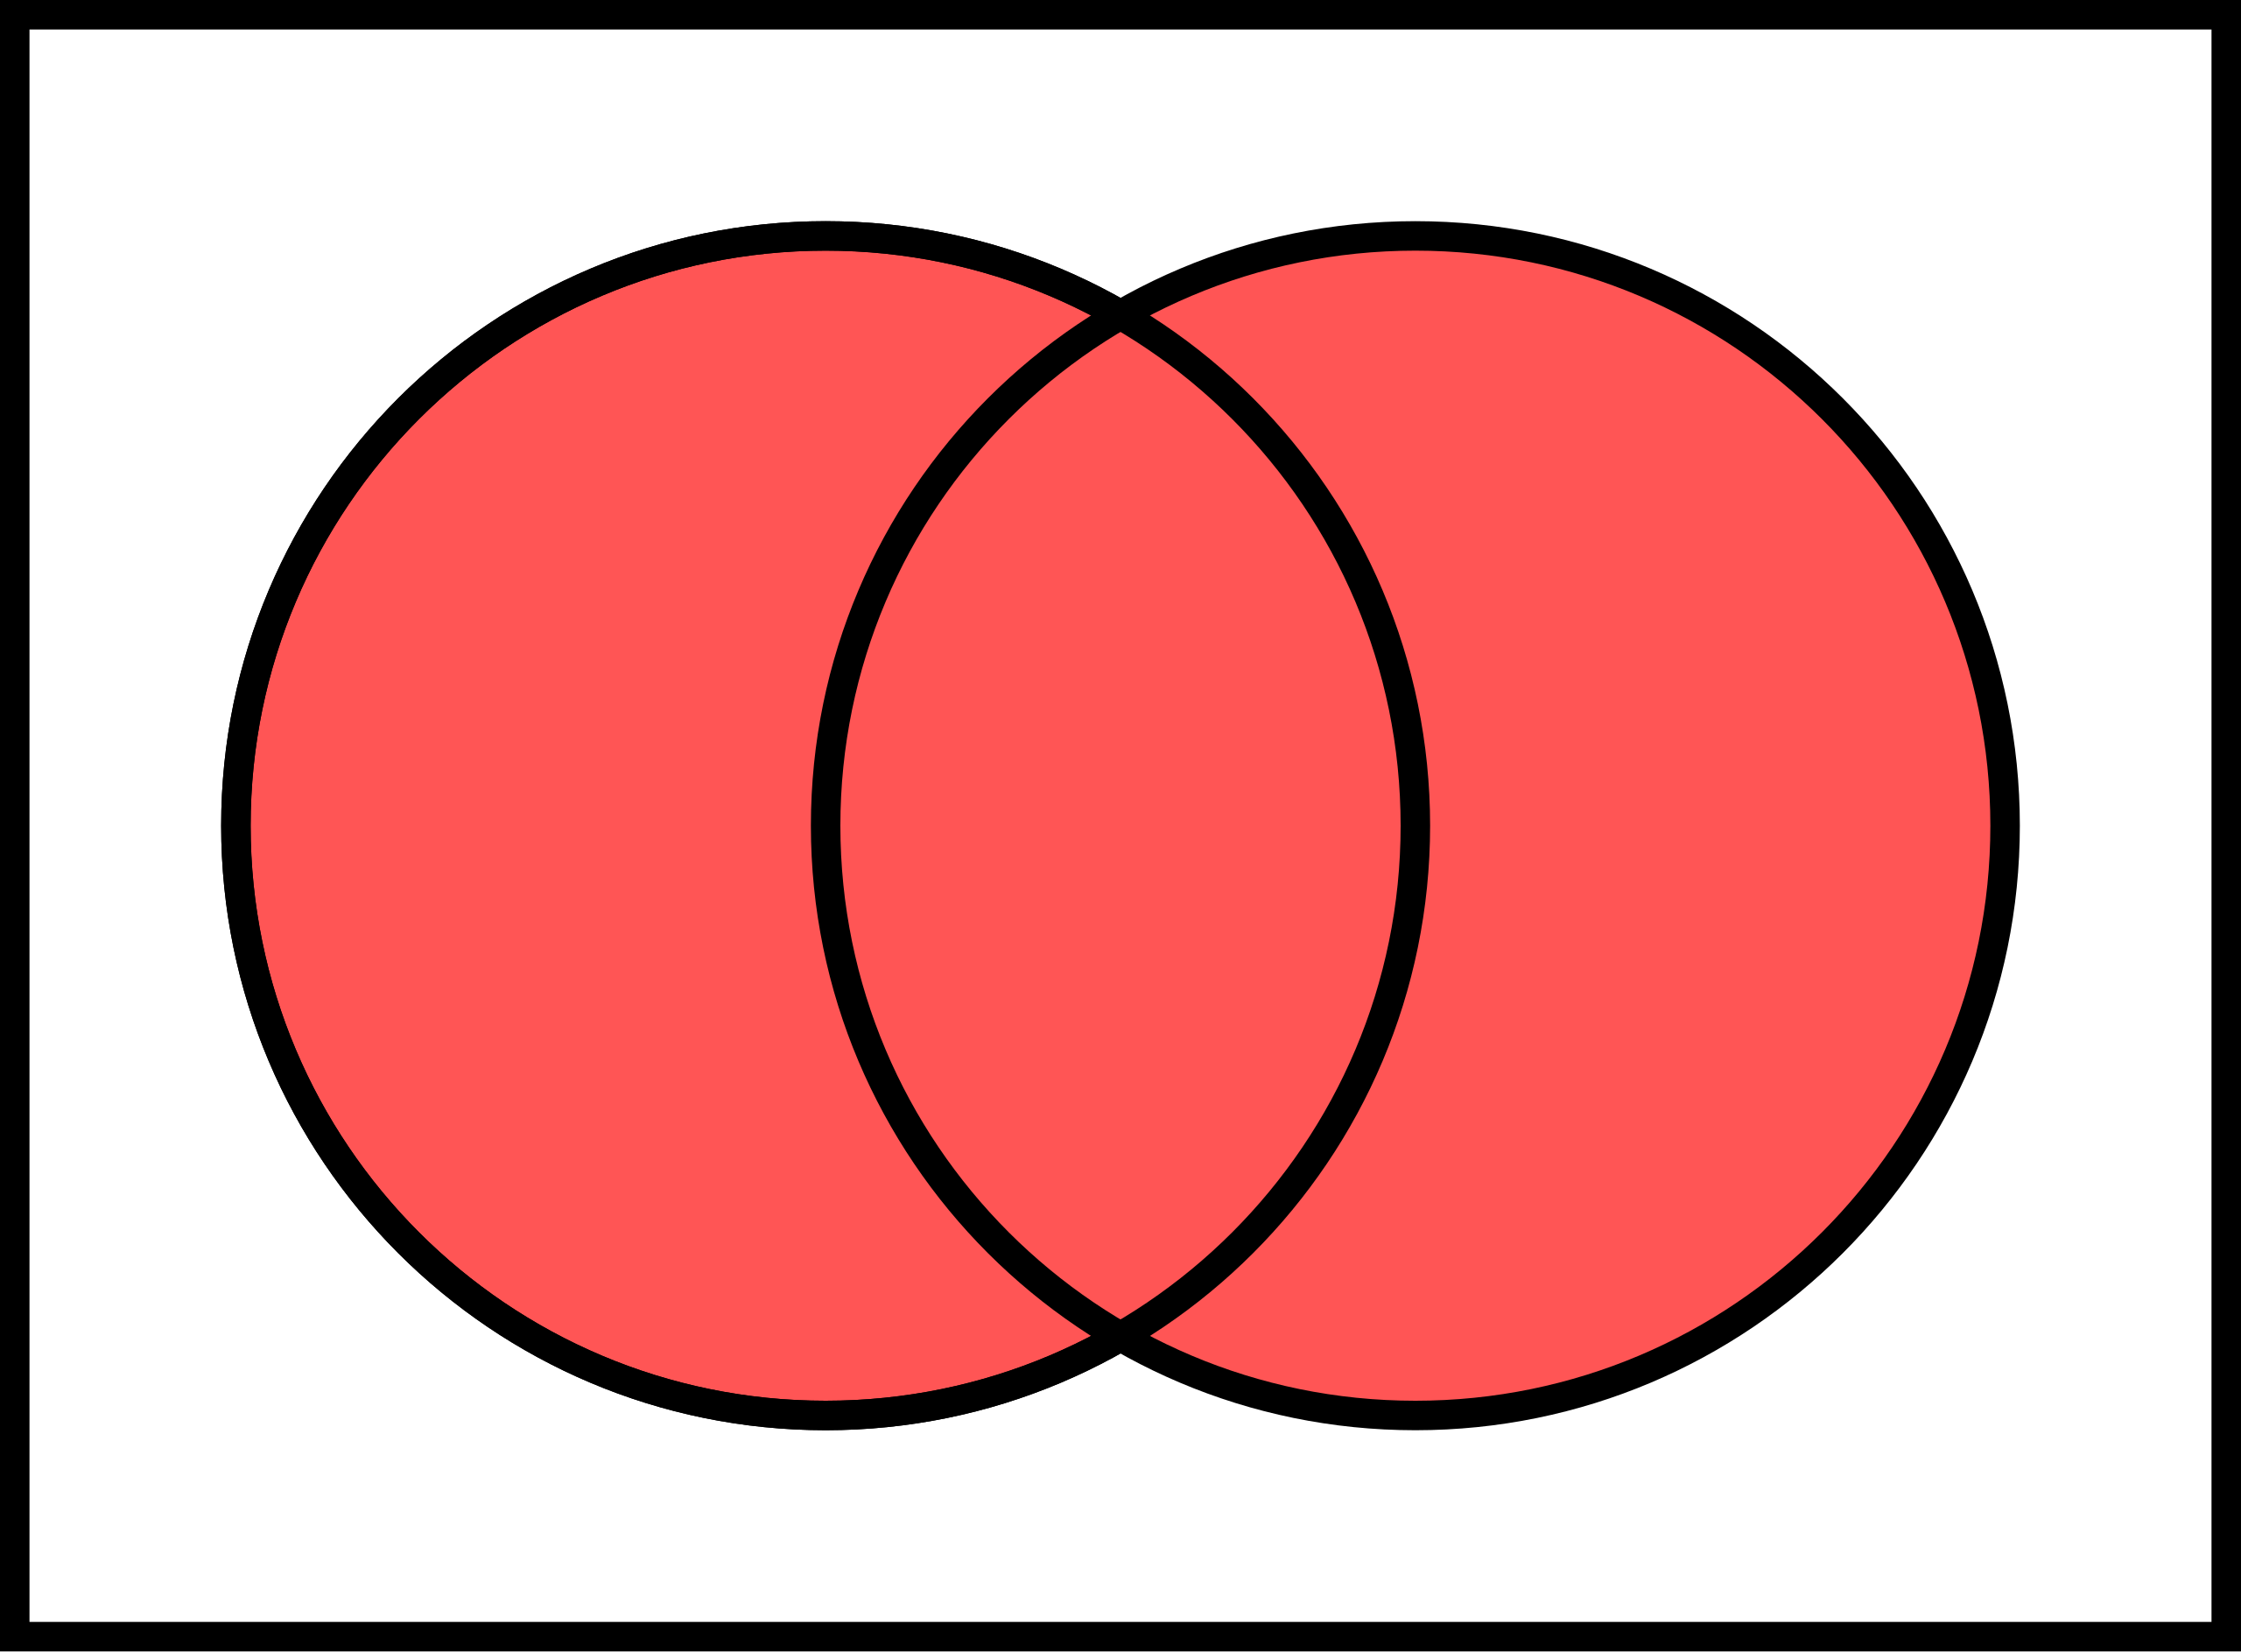
\includegraphics[width=\textwidth]{images/Venn0111.png}
    \caption{union}
  \end{minipage}
  \hfill
  \begin{minipage}[t]{0.4\textwidth}
    \centering
    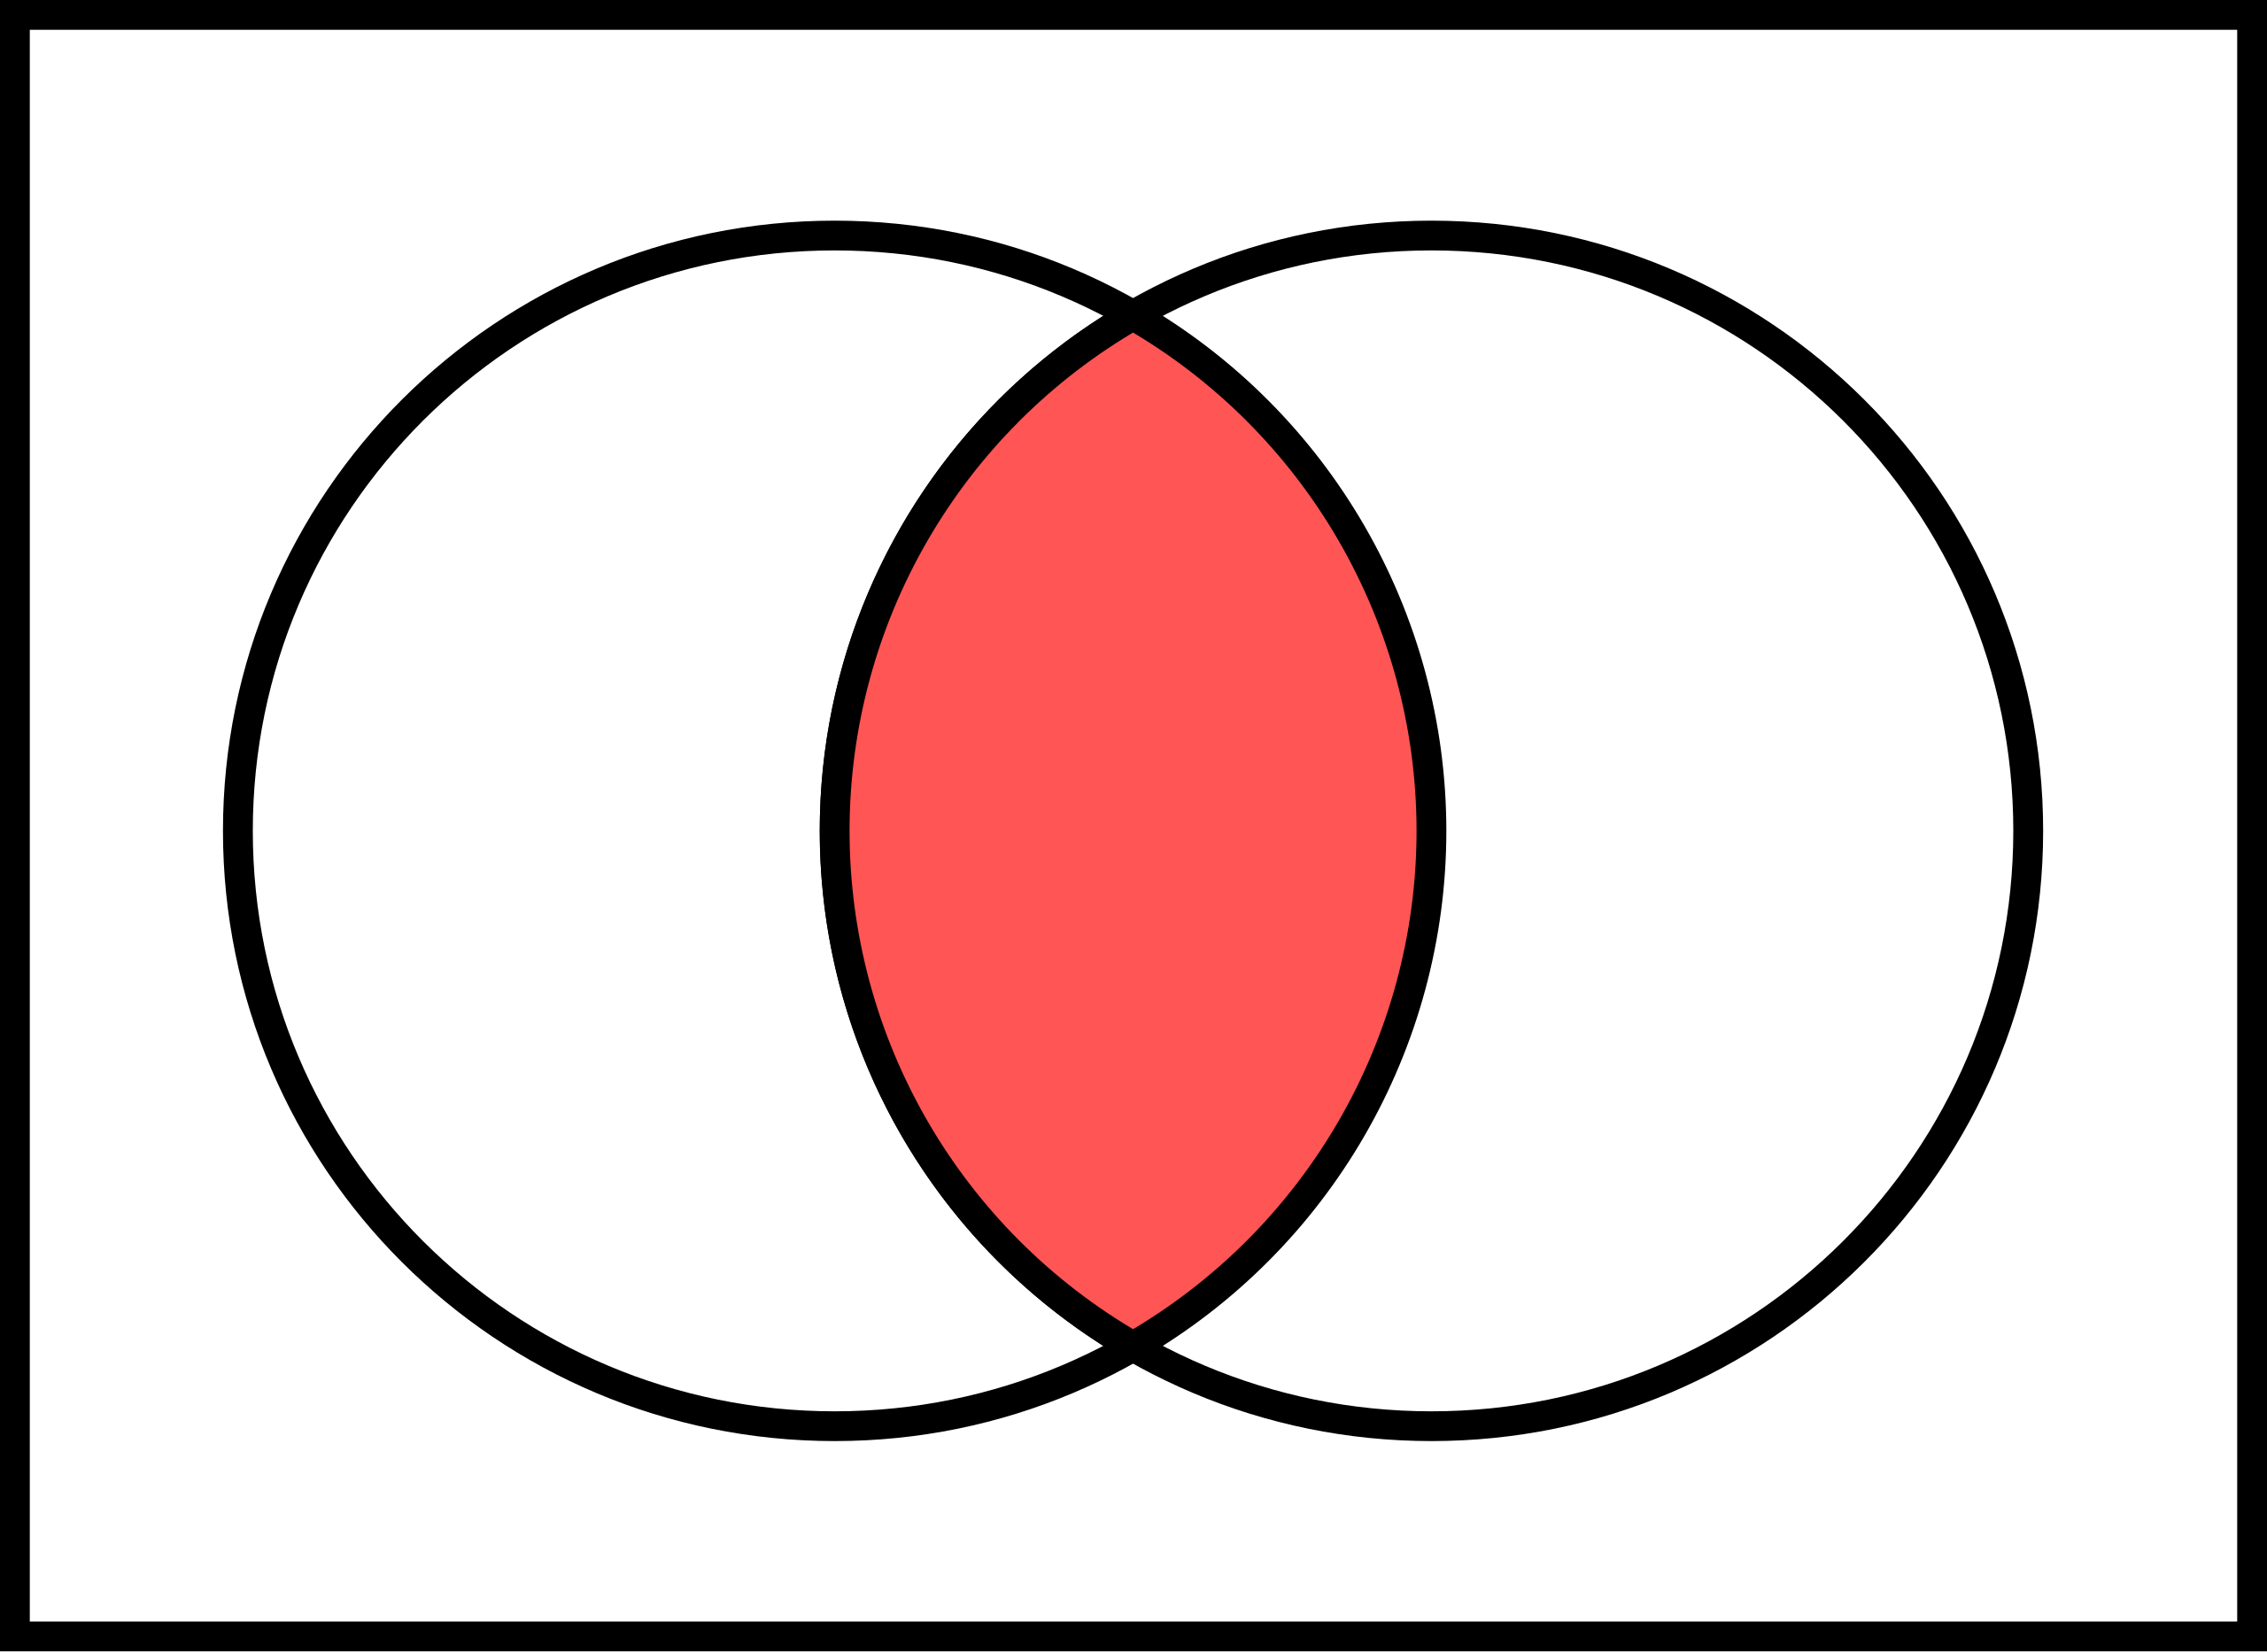
\includegraphics[width=\textwidth]{images/Venn0001.png}
    \caption{intersection}
  \end{minipage}
  \vspace{1em}
  \begin{minipage}[t]{0.4\textwidth}
    \centering
    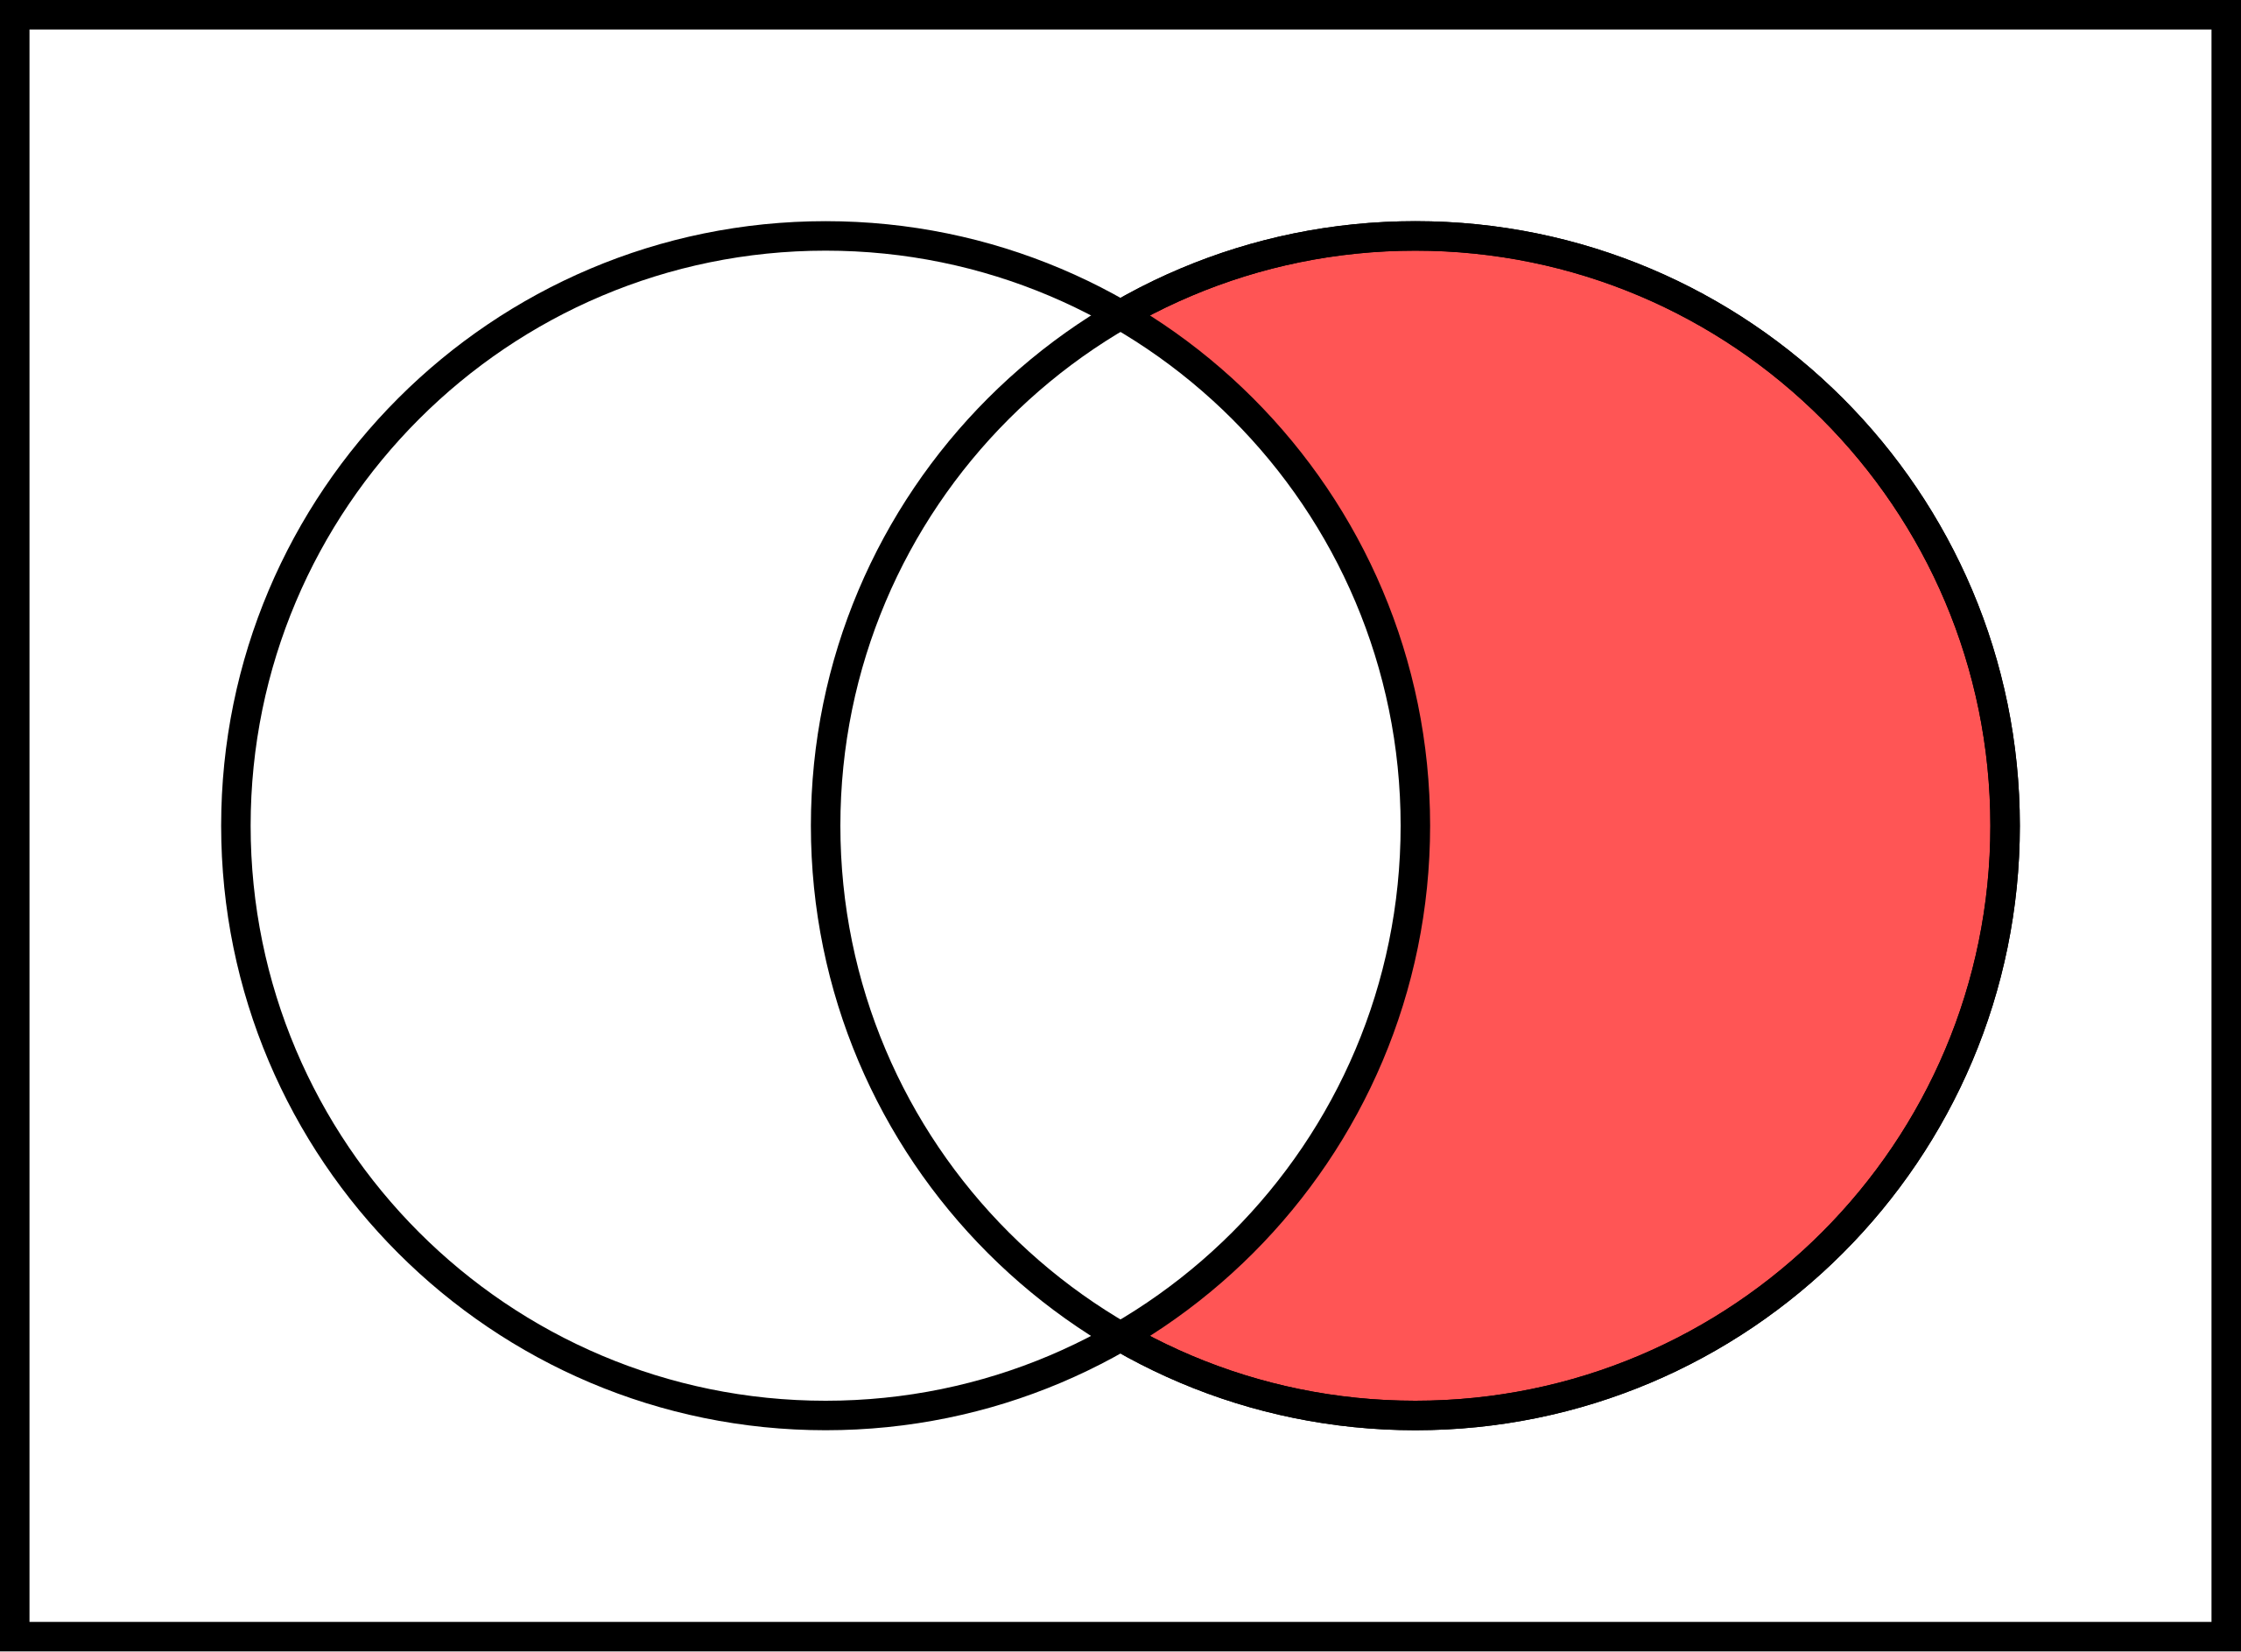
\includegraphics[width=\textwidth]{images/Venn004.png}
    \caption{difference}
  \end{minipage}
  \hfill
  \begin{minipage}[t]{0.4\textwidth}
    \centering
    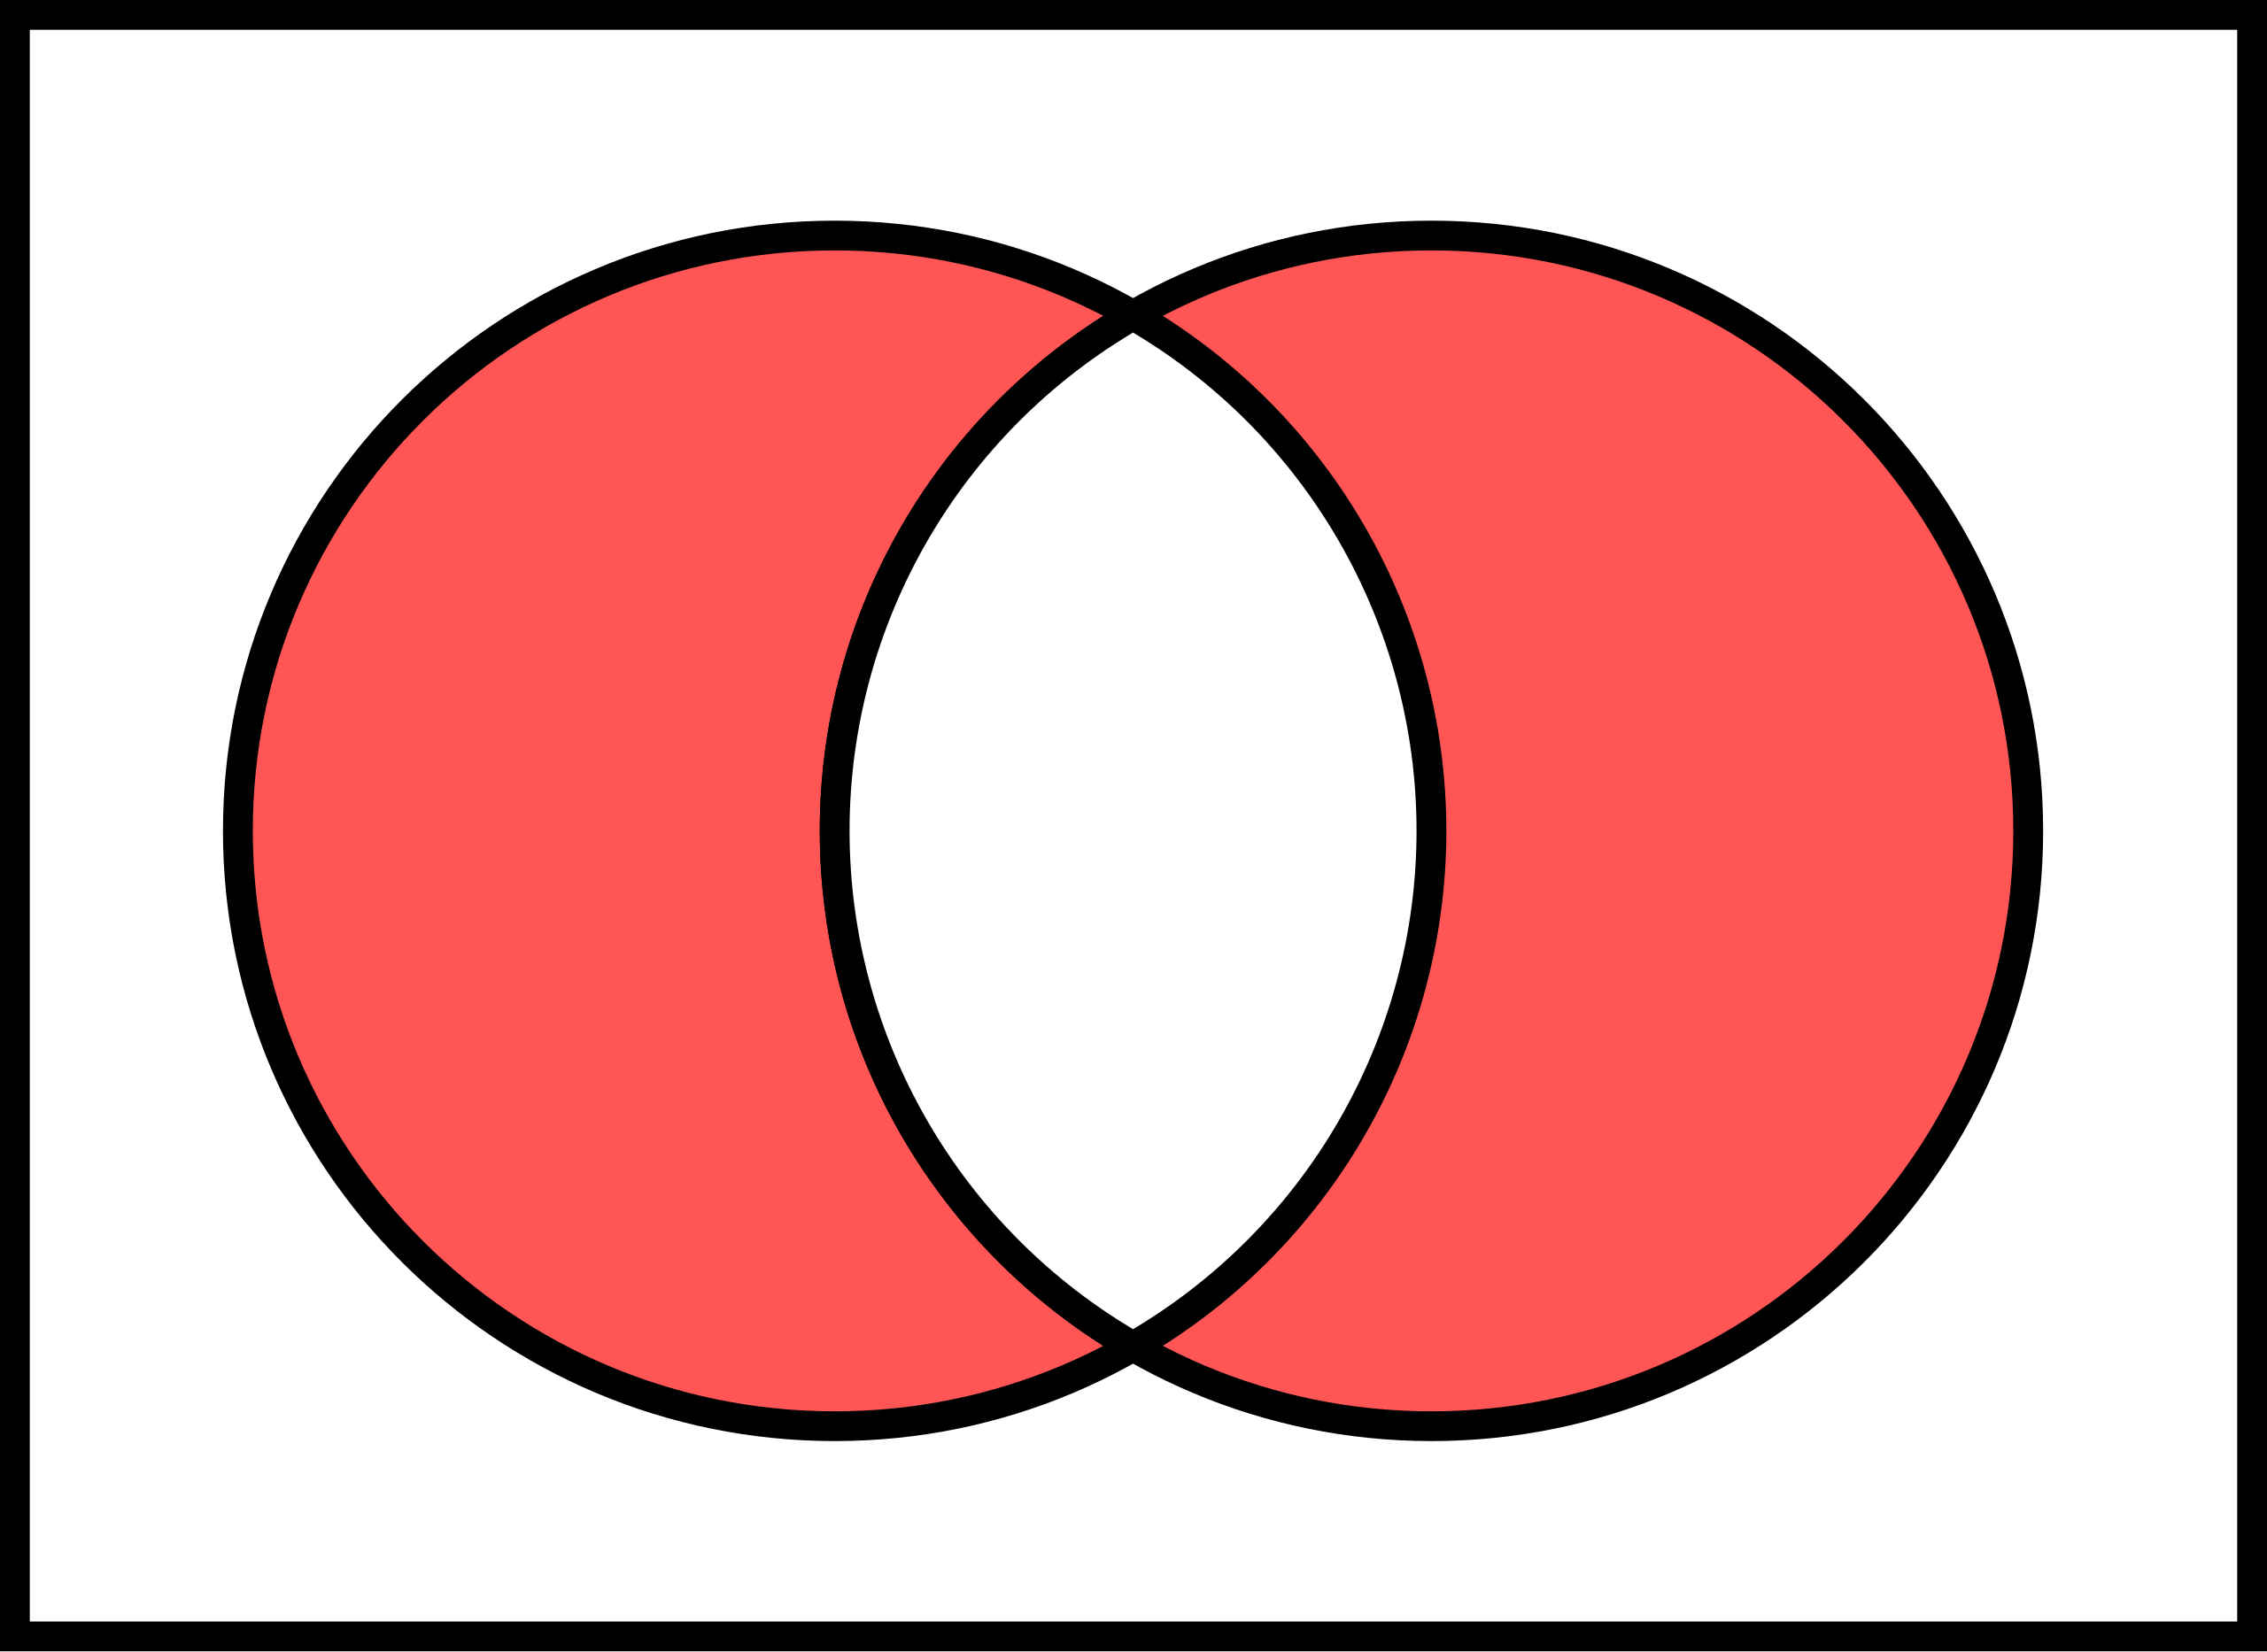
\includegraphics[width=\textwidth]{images/Venn003.png}
    \caption{symmetric difference}
  \end{minipage}
\end{figure}

\begin{remark}
  Union and intersection can also be defined for any amounts of sets by using index set. Let $E$ be a set. $\forall \alpha \in E$, we associate it with a set $A_{\alpha}$ and then define $\bigcup_{\alpha \in E} A_{\alpha}$ and $\bigcap_{\alpha \in E} A_{\alpha}$.
\end{remark}

\underline{Notation}: $\bigsqcup_{\alpha \in E} A_{\alpha}$ means disjoint union, i.e. $\forall \alpha, \beta \in E, \alpha \neq \beta$, we have $A_{\alpha} \cap A_{\beta} = \emptyset$.

\begin{proposition}
  \begin{enumerate}
    \item Commutativity: $A \cup B = B \cup A$, $A \cap B =B \cap A$;
    \item Associativity: $(A \cup B) \cup C = A \cup (B \cup C)$, $(A \cap B) \cap C = A \cap (B \cap C)$;
    \item Distributivity: $A \cup (B \cap C) = (A \cup B) \cap (A \cup C)$, $A \cap (B \cup C) = (A \cap B) \cup (A \cap C)$;

          \underline{Note}: If we view $\cup$ as $\oplus$ and $\cap$ as $\otimes$, then we get aioms of a commutative ring in algebra.

    \item De Morgan's Laws: $(\bigcup_{\alpha \in E} A_{\alpha})^c = \bigcap_{\alpha \in E} A_{\alpha}^c$, $(\bigcap_{\alpha \in E} A_{\alpha})^c = \bigcup_{\alpha \in E} A_{\alpha}^c$.
          \begin{proof}
            Let $\Omega$ be the whole space. We only prove the first identity.

            1. $\forall x \in LHS$, $x \in \Omega$ and $x \notin \bigcup_{\alpha \in E} A_{\alpha}$

            $\Rightarrow \forall \alpha \in E, x \notin A_{\alpha} \Rightarrow \forall \alpha \in E, x \in A_{\alpha}^c \Rightarrow x \in \bigcap_{\alpha \in E} A_{\alpha}^c$.

            2. $\forall x \in RHS$, $\forall \alpha \in E, x \in A_{\alpha}^c$ and $x \notin \bigcap_{\alpha \in E} A_{\alpha}^c$.

            $\Rightarrow \forall \alpha \in E, x \in A_{\alpha} \Rightarrow \forall \alpha \in E, x \in A_{\alpha}^c \Rightarrow x \in \bigcup_{\alpha \in E} A_{\alpha}^c$.

            Thus, $LHS = RHS$.
          \end{proof}
  \end{enumerate}
\end{proposition}

\begin{definition}[Cartesian Product]\index{Cartesian Product}

  Let $A, B$ be two sets, then the \textbf{Cartesian Product} of $A$ and $B$ is defined as $A \times B = \{(a, b): a \in A, b \in B\}$.
\end{definition}

\begin{example}
  $\R^2 = \R \times \R$, $R^n = \underbrace{R \times R \times \dots \times R}_{\text{n times}}$.
\end{example}

\clearpage

\subsection{Functions between Sets}

\subsubsection{Mappings, Functions}

\begin{definition}[Function]\index{Function}

  Let $A, B$ be two sets, then a \textbf{mapping} is a set $X \subset A \times B$, s.t.

  1. $\forall x \in X$, $\exists y \in B$, s.t. $(x, y) \in X$;

  2. $\forall x \in A$, $\forall y_1, y_2 \in B$, if $(x, y_1) \in X$ and $(x, y_2) \in X$, then $y_1 = y_2$.

  Such a mapping is called a \textbf{function}.
\end{definition}

\underline{Notation}: $y = f(x)$ (function $\leftrightarrow mapping$).

\begin{definition}
  \begin{enumerate}
    \item \textbf{Injective}: $f(x_1) = f(x_2) \Rightarrow x_1 = x_2$.
    \item \textbf{Surjective}: $\forall y \in B, \exists x \in A$, s.t. $f(x) = y$.
    \item \textbf{Bijective}: both injective and surjective.

          (bijection $\leftrightarrow$ equivalence $\leftrightarrow$ one-to-one mapping)
  \end{enumerate}
\end{definition}

\subsubsection{Equivalence Relations}

\begin{definition}[Equivalence Relation]\index{Equivalence Relation}

  Let $A$ be a set, then an \textbf{equivalent realtion} on $A$ is a subset $X \subset A \times A$, with the following properties:

  (\underline{Notation}: $x \sim y$ if $(a, b) \in X$)

  1. reflexivity: $x \sim x$;

  2. symmetry: $x \sim y \Rightarrow y \sim x$;

  3. transitivity: $x \sim y, y \sim z \Rightarrow x \sim z$.
\end{definition}

\begin{definition}
  Having an equivalent relation, an \textbf{equivalent class} of an element $x \in A$ is defined as $[x] := \{y \in A: y \sim x\}$.
\end{definition}

\begin{proposition}
  Two equivalent classes either coincide or don't intersect.
\end{proposition}

\begin{theorem}
  $\exists$ a set $E \subset A$, s.t. $A = \bigsqcup_{\alpha \in E} X_{\alpha}$, i.e $A$ is a disjoint union of equivalent classes.
\end{theorem}

Thus, each equivalent class can uniquely identified by randomly selecting one element from the class, which is called a \textbf{representative} of the equivalent class.

\begin{example}
  Let $A = \C$: the complex plain. $z \sim w$ if $|z| = |w|$.

  Then $\C = \bigsqcup_{r \in [0, + \infty)} C_r$, where $C_r = \{ z \in \C: |z| = r\}$.
\end{example}

\begin{definition}
  Two sets $A, B$ are called \textbf{equivalent} if there exists a bijection $f: A \rightarrow B$.
\end{definition}

From now on, we focus on equivalence relation of sets based on the above definition.

\subsubsection{Cardinals, Countable Sets}

\begin{definition}[Cardinal]\index{Cardinal}

  Let $X$ be a set of sets. This gives an equivalent relation on $X$. We obtain equivalent classes of sets. Each equivalent class is called a \textbf{cardinal (cardinal number)}.
\end{definition}

\underline{Notation}: $|A|$: cardinal of set $A$.

\begin{remark}
  1. Define $"0"$ = emptyset, $"1"$ = $\{0\}$, $"2"$ = $\{0,1\}$, $"3"$ = $\{0,1,2\}$, etc. So, the number $"n"$ is really a set with $n$ elements in it.

  2. A set $A$ is called "finite" iff there is some $n$ and a function $f: A \rightarrow \{1, 2, \ldots, n\}$ which is bijective.

  3. A set $A$ is called "infinite" iff it is not finite.
\end{remark}

\begin{example}
  $A = \{a_1, a_2, \ldots, a_n\}, B = \{b_1, b_2, \ldots, b_m\}$, then $A \sim B \Leftrightarrow n = m$.
\end{example}

\begin{definition}[Countable Set]\index{Countable Set}

  A set $A$ is called \textbf{countable} if $A \sim \N$.

  A countable set is also called \textbf{listable}, which means we can list all its elements in an infinite sequence.
\end{definition}

So, the key to prove a set is countable is

1. to find a bijection between the set and $\N$;

or

2. to find a way to explicitly list out all elements of the set without repeating or missing a single element.

\begin{definition}[At Most Countable Set]\index{At Most Countable Set}

  A set $A$ is called \textbf{at most countable} if $A$ is finite or countable.
\end{definition}


\begin{proposition}
  A set $A$ is infinite $\Leftrightarrow A \supset B$, where $B$  is a countable set.
  \begin{proof}
    $\Leftarrow$: Obvious;

    $\Rightarrow$: Take $a_1 \in A$, then take $A \setminus \{a_1\}$ which is also infinite. So we can take $a_2 \in A \setminus \{a_1\}$, then take $A \setminus \{a_1, a_2\}$ which is also infinite. Repeat this process.

    Let $B = \{a_1, a_2, a_3, \ldots\}$ where all $a_i$ are distinct $\Rightarrow A \supset B$.
  \end{proof}
\end{proposition}

\clearpage

\subsection{Standard Equivalences}

\subsubsection{Important Examples}

\begin{example}
  \begin{enumerate}
    \item $\Z \sim \N$
          \begin{proof}
            We just list all the elements of $Z$: $\Z = \{0, 1, -1, 2, -2, \ldots\}$.
          \end{proof}
    \item $\Q \sim \N$
          \begin{proof}
            \[\begin{array}{c|ccccc}
                       & 1      & 2      & 3      & 4      & \cdots \\ \hline
                1      & 0/1    & 1/1    & 2/1    & 3/1    & \cdots \\
                2      & 0/2    & 1/2    & 2/2    & 3/2    & \cdots \\
                3      & 0/3    & 1/3    & 2/3    & 3/3    & \cdots \\
                4      & 0/4    & 1/4    & 2/4    & 3/4    & \cdots \\
                \vdots & \vdots & \vdots & \vdots & \vdots & \ddots
              \end{array}\]

            Start from $(1,1)$ and move along the diagonals:
            \((1,1),\ (1,2),(2,1),\ (3,1),(2,2),(1,3),\ldots\) while we skip those fractions that are not in the lowest terms (repeated).

            This gives us the following sequence:
            \( \frac{0}{1}, \frac{1}{1}, \frac{1}{2}, \frac{2}{1}, \frac{3}{1}, \frac{1}{3}, \frac{2}{3}, \frac{3}{2}, \frac{4}{1}, \ldots\) which is a listing of all positive elements in $\Q$. Then, using the same trick to deal with all the negative elements as we listing all elements in $\Z$, we have $\Q \sim \N$.
          \end{proof}
    \item $\R \sim (0,1)$
          \begin{proof}
            1. $(a,b) \sim (c,d)$: $y = \alpha x + \beta$;

            2. $f(x) = arctan(x)$: $\R \rightarrow (-\frac{\pi}{2}, \frac{\pi}{2})$.

            Composing 1 and 2, we can get $\R \sim (0,1)$.
          \end{proof}
    \item $(a,b) = [a,b]$
          \begin{proof}
            We only need to prove $(0,1) \sim [0,1]$.

            Define $f(x) = \begin{cases} \frac{1}{2}, & x = 0; \\ \frac{1}{3}, & x = 1; \\ \frac{1}{n+2}, & x = n \in \N; \\ x, & \text{otherwise}; \end{cases}$

            It is easy to check that $f$ is bijective.
          \end{proof}
  \end{enumerate}
\end{example}

\subsubsection{Continual Sets, Cantor's Theorem}

\begin{definition}[Continual Set]\index{Continual Set}

  A set $A$ is called \textbf{continual} if $A \sim \R$.
\end{definition}

\begin{remark}
  continual sets $\sim \R \sim [a,b] \sim (a,b)$.
\end{remark}

\underline{Question}: Is continual the same as uncountable?

\begin{theorem}[Cantor's Theorem]\index{Cantor's Theorem}

  $\forall$ set $E$: $E \not\sim 2^E$.
  \begin{proof}
    Assume rather: $\exists$ a bijection $f : E \rightarrow 2^E$.

    Consider $A = \{x \in E: x \notin f(x) \in 2^E\} \subset E \Rightarrow A \in 2^E$.

    Since $f$ is bijctive, there exists a unique $a \in E$ s.t. $A = f(a)$.

    \underline{Question}: Is $a \in A$?

    1. If $a \in A$, then by definition of $A$, $a \notin f(a) = A$. Contradiction.

    2. If $a \notin A$, then by definition of $A$, $a \in f(a) = A$. Contradiction.

    So such bijection $f$ doesn't exist $\Rightarrow E \not\sim 2^E$.
  \end{proof}
\end{theorem}

Now, let's consider $2^\N$.

In fact, $2^\N \sim \{$ all sequences of $\{0,1\}$ $\}$ (each 0 and 1 meaning whether en element in $\N$ is in the subset or not).

\underline{Reminder}: $\forall x \in [0,1]$, $x$ can be written as $x = 0. a_1 a_2 a_3 \dots$, with $a_n \in \{0,1\} \forall n$.

Method: Using bisection method, if $x \in [0, \frac{1}{2}) \Rightarrow a_1 =0$, if $x \in [\frac{1}{2}, 1] \Rightarrow a_1 = 1$. Repeat this process for each subinterval.

      For example, $1 = 0.111111\dots$.

      And this method of representing all elements in $[0,1]$ can cover all elements in $\{$ all sequences of $\{0,1\}$ $\}$. Also, we don't have two elements in $[0,1]$ corresponding to the same sequence of $\{0,1\}$ except those like $0.1000\dots = 0.0111\dots$. These elements are countable, so we can just ignore them (Countable sets setminus countable real subsets can still have at most countable elements left).

      Thus, $2^\N \sim [0,1]$ and $2^\N \not\sim \N$.

    $\Rightarrow$ continual $\not=$ countable.

      \begin{remark}
        We can represent the cardinal of countable and continual sets by using Hebrew alphabet $\aleph_0$ and $\aleph_1$, i.e. $|\N| = \aleph_0, |\R| = \aleph_1$.
      \end{remark}

      \clearpage

      \subsection{Comparing Cardinals}

      \subsubsection{Ordered Sets}

      \begin{definition}[Order]\index{Order}

        Let $E$ be a set, then an \textbf{order (partial order)} on $E$ is a subset $X \subset E \times E$, we write $a \leq b$ with the following properties:

        (\underline{Notation}: if $(a,b) \in X$)

        1. reflexivity: $a \leq a$;

        2. anti-symmetry: $a \leq b$ and $b \leq a \Rightarrow a = b$;

        3. transitivity: $a \leq b$ and $b \leq c \Rightarrow a \leq c$.

        $E$ is called a \textbf{(partial) ordered set} with order $\leq$.
      \end{definition}

      \begin{example}
        \begin{enumerate}
          \item $\R$: natural ordering. Take $E \subset \R$.
          \item $\R^n$ with lexicographic ordering:

                $\vec{x} = (x_1, \ldots, x_n), \vec{y} = (y_1, \ldots, y_n)$, then $\vec{x} \leq \vec{y}$ means $x_i \leq y_i, \forall i \in \llbracket 1, n \rrbracket$

                Note that not all elements are comparable, e.g. $(1,2)$ and $(2,1)$ are not comparable.
        \end{enumerate}
      \end{example}

      \begin{definition}[Linearly Ordered Set]\index{Linearly Ordered Set}

        We add the forth axiom to the definition of order:

        4. comparability: $\forall a,b \in E$, it holds $a \leq b$ or $b \leq a$.

        Then $E$ is called a \textbf{linearly ordered set} with order $\leq$.
      \end{definition}

      \begin{example}
        Still take $E \subset \R$.
      \end{example}

      \begin{definition}[Well Ordered Set]\index{Well Ordered Set}

        We add the fifth axiom to the definition of linearly ordered set:

        5. least element: $\forall A \subset E$, $A$ has its \textbf{least element}, i.e. $\exists a \in A$, s.t. $a \leq x, \forall x \in A$.

        Then $E$ is called a \textbf{well ordered set} with order $\leq$.
      \end{definition}

      \begin{example}
        $\N$ with the usual order.
      \end{example}

      \begin{example}\underline{A linearly ordered set but not a well ordered set}

        $\Z$ with the usual order.

        $\Z_{<0} \subset \Z$ but it doesn't have a least element.
      \end{example}

      \subsubsection{Zermelo's theorem, Cantor-Bernshtain Theorem}

      The sets of all cardinals actually can have order, which follows our intuition.

      \begin{definition}
        For two cardinals $C_1$ and $C_2$, we say that $C_1 \leq C_2$ if for some representative set $E_1 \in C_1$ and $E_2 \in C_2$, it holds $E_1 \sim E_2^{\prime} \subset E_2$ for some $E_2^{\prime} \subset E_2$.
      \end{definition}

      \begin{example}
        Natually, $\aleph_0 \leq \aleph_1$ since $\N \sim \N \subset \R$.
      \end{example}

      \begin{theorem}[Zermelo's Theorem]\index{Zermelo's Theorem}

        $\forall$ cardinals $C_1, C_2$, it holds: either $C_1 \leq C_2$ or $C_2 \leq C_1$, i.e. $\forall$ set $A, B$, either $A \sim B^{\prime} \subset B$ or $B \sim A^{\prime} \subset A$.
      \end{theorem}

      \begin{theorem}[Cantor-Bernstein Theorem]\index{Cantor-Bernstein Theorem}

        If $|X| \leq |Y|$, and $|Y| \leq |X|$, then $|X| = |Y|$.
        \begin{proof}
          Let $f: X \to Y$ and $g: Y \to X$ be injections.

          Consider a point $x \in X$.
          \begin{itemize}
            \item If $x \in g(Y)$, we form $g^{-1}(x) \in Y$.
            \item If $g^{-1}(x) \in f(X)$, we form $f^{-1}(g^{-1}(x))$, and so forth.
          \end{itemize}
          Either this process can be continued indefinitely, or it terminates with an element of $X \setminus g(Y)$, or $Y \setminus f(X)$.

          In these 3 cases we say that $x$ is in $X_{\infty}$, $X_X$ or $X_Y$.
          $$\implies X = X_{\infty} \sqcup X_X \sqcup X_Y.$$

          In the same way, $Y = Y_{\infty} \sqcup Y_X \sqcup Y_Y$.

          Clearly, $Y_X \stackrel{f}{\leftrightarrow} X_X$, $Y_Y \stackrel{g}{\leftrightarrow} X_Y$. We claim that $X_{\infty} \stackrel{f}{\leftrightarrow} Y_{\infty}$ also holds.

          It is an injection between $X_{\infty}$ and $Y_{\infty}$ by its definition. And if we consider any $y$ in $Y_{\infty}$, it means we can track an infinite chain by looking for the preimage. Let the first preimage of $y$ be $x$, then $x$ also has an infinite chain, inheriting from $y$, and thus is in $X_\infty$. Thus, $f$ is also a surjection between $X_{\infty}$ and $Y_{\infty}$.

          Therefore we define $h: X \to Y$ by
          $$h(x) = \begin{cases}
              f(x)      & \text{if } x \in X_{\infty} \cup X_X \\
              g^{-1}(x) & \text{if } x \in X_Y
            \end{cases}$$

          \noindent Then $h$ is bijective.
        \end{proof}
      \end{theorem}

      \begin{corollary}
        The set of all cardinal numbers is linearly ordered.
      \end{corollary}

      Further, we have the theorem below also by Zermelo.

      \begin{theorem}[Zermelo's Theorem]\index{Zermelo's Theorem}
        Cardinal numbers are actually well ordered.
      \end{theorem}

      So, one can natually order cardinals.

      \clearpage

      \subsection{Continuum Hypothesis and Exercises}

      Cantor Theorem means $|E| < |2^E| \implies \exists$ larger and larger cardinals.

      For example, $|\N| = \aleph_0 < |\R| = \aleph_1$.

      \subsubsection{Continuum Hypothesis}

      \underline{Famous Open Question: Continuum Hypothesis}\index{Continuum Hypothesis}

      We know that $\aleph_0 < \mathfrak{c}$ (where $\mathfrak{c} = 2^{\aleph_0}$).

      \underline{Question}: Does there exist a set $A$ such that $\aleph_0 < |A| < \mathfrak{c}$?

      \begin{theorem}
        This question has no solution! (i.e. the existence of such set cannot be proved or disproved). This is an illustration of G\"odel's Incompleteness Theorem.
      \end{theorem}


      \subsubsection{A Few Exercises}

      \begin{example}
        Prove $\R \setminus \N \sim \R$.
        \begin{proof}
          Clearly, $\R \setminus \N \subset \R$.
          On the other hand, $\R \setminus \N \supset (0,1) \sim \R$.
          By Cantor-Bernstein Theorem: $\R \setminus \N \sim \R$.
        \end{proof}
      \end{example}

      \begin{example}
        Prove that $C[0,1] \sim \R$, where $C[0,1]$ is the space of continuous functions on $[0,1]$.
        \begin{proof}
          Reason: A continuous function is uniquely determined by its values at $x \in \Q$!
          ($f(x) = \lim_{x_n \to x, x_n \in \Q} f(x_n)$).

          Thus, $|C[0,1]| \leq |\{f: \Q \cap [0,1] \to \R\}|$.
          Let's analyze this cardinality.
          $|\{f: \Q \to \R\}| = |\R^\Q| = (\mathfrak{c})^{\aleph_0} = (2^{\aleph_0})^{\aleph_0} = 2^{\aleph_0 \cdot \aleph_0} = 2^{\aleph_0} = \mathfrak{c} = |\R|$.

          On the other hand, constant functions are in $C[0,1]$, so $\R \subset C[0,1] \implies |\R| \leq |C[0,1]|$.

          By Cantor-Bernstein Theorem, $|C[0,1]| = \mathfrak{c} = |\R|$.
        \end{proof}
      \end{example}

      \clearpage

      \subsection{Axiom of Choice and Zorn's Lemma}

      \begin{definition}[Axiom of Choice]\index{Axiom of Choice}
        Let $\{A_\alpha\}_{\alpha \in I}$ be a group of sets (meaning a family of sets indexed by $I$).
        Then there exists a function $f: I \to \bigcup_{\alpha \in I} A_\alpha$ such that $f(\alpha) \in A_\alpha$ for all $\alpha \in I$.
        (This essentially means we can "choose" one element from each set simultaneously).
      \end{definition}

      This axiom has several equivalent formulations, and the most applicable one is as follows:

      \begin{theorem}[Zorn's Lemma]\index{Zorn's Lemma}
        Let $E$ be a (partially) ordered set. Assume that the followings hold:
        Every \textbf{chain} $A$ in $E$ (i.e. a subset $A \subset E$ where every 2 elements are comparable) has an upper bound in $E$ (i.e. $\exists s \in E$ s.t. $x \leq s, \forall x \in A$).

        Then $E$ has a \textbf{maximal element} $m$ (i.e. $\nexists x \in E$ s.t. $m < x$, or equivalently $\forall x \in E, m \leq x \implies m = x$).
      \end{theorem}

      \begin{remark}
        Axiom of Choice $\iff$ Zorn's Lemma.
      \end{remark}

      One application of Zorn's Lemma is the existence of a basis in a linear space (even infinite-dimensional).

      \begin{definition}[Basis of a Linear Space]\index{Basis of a Linear Space}
        A basis for a linear space $V$ is a system $S = \{e_\alpha\}$ such that:
        \begin{enumerate}
          \item There are no (finite) non-trivial linear combinations between elements of $\{e_\alpha\}$ equal to 0 (i.e. $\{e_\alpha\}$ are linearly independent).
          \item Any $x \in V$ is a (finite) linear combination of elements of $\{e_\alpha\}$.
        \end{enumerate}
      \end{definition}

      \begin{remark}
        Generally there is no way to see (construct) a Hamel basis.
      \end{remark}

      \begin{theorem}
        Any linear space $V$ admits a Basis (called the \textbf{Hamel basis}).
        \begin{proof}
          Let $E = \{ \text{the set of all linearly independent systems of vectors in } V \}$.
          Let's introduce ordering on $E$:
          $S_1 \leq S_2 \iff S_1 \subset S_2$.
          It is easy to check that we've got a partial order.

          Now, let's check that the conditions of Zorn's Lemma are satisfied.
          Take a chain $\{S_\alpha\}_{\alpha \in A} \subset E$.
          Then $\{S_\alpha\}$ has an upper bound: $S = \bigcup_{\alpha \in A} S_\alpha$.
          Then $S$ is also a linearly independent system.
          (Why? Any finite linear combination in $S$ involves finite elements, which must all belong to some $S_{\alpha_0}$ because $\{S_\alpha\}$ is a chain. Since $S_{\alpha_0}$ is lin. indep., the combination is trivial.)
          $S$ is clearly an upper bound for $\{S_\alpha\}$.

          By Zorn's Lemma, $\exists S_0$ - a maximal linearly independent system.
          We claim $S_0$ is a basis.
          If not, $\exists x \in V$ which is not in the span of $S_0$.
          Then $S_0 \cup \{x\}$ is a strictly bigger lin. indep. system.
          This contradicts the maximality of $S_0$.
          $\implies S_0$ is a basis.
        \end{proof}
      \end{theorem}

      \clearpage


      \section{Metric Space}

      \clearpage

      \subsection{Metric Space and Normed Space}

      \begin{definition}[Metric Space]\index{Metric Space}
        A \textbf{metric space} is a set $X$ equipped with a given $\rho: X \times X \to \R$ (\textbf{distance function (metric)}) with the following properties:
        \begin{enumerate}
          \item $\rho(x, y) \geq 0$ and $\rho(x, y) = 0 \iff x = y$ (\textbf{nondegeneracy}).
          \item $\rho(x, y) = \rho(y, x)$ (\textbf{symmetry}).
          \item $\rho(x, y) \leq \rho(x, z) + \rho(z, y), \forall x, y, z \in X$ (\textbf{triangle inequality}).
        \end{enumerate}
      \end{definition}

      \begin{example}
        \begin{enumerate}
          \item $X = \R, \rho(x, y) = |x - y|$.
          \item Any set $E$ with $\rho(x, y) = \begin{cases} 1, & x \neq y \\ 0, & x = y \end{cases}$.
        \end{enumerate}
      \end{example}

      \begin{proposition}
        If $X$ is a metric space, $\forall Y \subset X$, $Y$ is also a metric space with the same $\rho$.
        \begin{example}
          $\N \subset \R$; $(a, b) \subset \R$.
        \end{example}
      \end{proposition}

      \begin{definition}[Normed Space]\index{Normed Space}
        A \textbf{normed space} is a linear space $X$ equipped with a function $\|\cdot\|: X \to \R$ with the following properties:
        \begin{enumerate}
          \item $\|x\| \geq 0$ and $\|x\| = 0 \iff x = 0$.
          \item $\|\alpha x\| = |\alpha| \|x\|, \forall x \in X, \alpha \in \R$.
          \item $\|x + y\| \leq \|x\| + \|y\|$ (indicating $\|x - y\| \leq \|x - z\| + \|z - y\|$).
        \end{enumerate}
      \end{definition}

      \underline{Fact}:
      A normed space is a metric space with $\rho(x, y) := \|x - y\|$.
      (For symmetry: $\|x - y\| = \|-(y - x)\| = |-1|\|y - x\| = \|y - x\|$).


      \begin{example}
        $\R^n$ with $\|x\| = \sqrt{\sum x_i^2}$.
        Accordingly defined scalar product in $\R^n$: $(x, y) = \sum x_i y_i$.
        Then $\|x\| = \sqrt{(x, x)}$.
        Triangle inequality: $\|x + y\| \leq \|x\| + \|y\| \iff (x+y, x+y) = (x, x) + (y, y) + 2(x, y) \leq \|x\|^2 + \|y\|^2 + 2\|x\|\|y\|$
        $\iff (x, y) \leq \sqrt{(x, x)(y, y)}$ (Cauchy-Schwarz Inequality).
      \end{example}

      \begin{remark}
        A more general fact is that any scalar product space (Euclidean space) is a normed space.
        So, $\R^n$ and all its subsets are metric spaces with
        $\rho(x, y) = \sqrt{\sum (x_i - y_i)^2}$.
      \end{remark}

      \begin{example}
        \begin{enumerate}
          \item $C[a, b] = \{ \text{cts. func. on } [a, b] \}$. $\|f\| = \max_{x \in [a, b]} |f(x)|$. $\rho$ accordingly defined.
          \item $\ell^2 = \{ \{x_j\} : \sum_{j=1}^\infty |x_j|^2 < \infty \}$.
          \item $X = \{ C[a, b], \text{but equipped with the norm } \|f\| := \int_a^b |f(x)| dx \}$.
        \end{enumerate}
      \end{example}

      \clearpage

      \subsection{Topology of Metric Spaces}

      \begin{definition}[Ball]\index{Ball}
        An \textbf{open ball} in a metric space $X$ with center $a \in X$ and radius $R > 0$:
        \[ B_R(a) = \{ x \in X : \rho(x, a) < R \}. \]
        \textbf{Closed ball}: $\bar{B}_R(a) = \{ x \in X : \rho(x, a) \leq R \}$.
      \end{definition}

      \begin{example}
        Any set $E$ with $\rho(x, y) = \begin{cases} 1, & x \neq y \\ 0, & x = y \end{cases}$.
        $B_{1/2}(a) = \{a\}, B_2(a) = E$.
      \end{example}

      \begin{example}
        $\R^n, B_1(0)$: Euclidean.
        $\|x\| = \max |x_i|$ (cube).
        $\|x\| = \sum |x_i|$.
      \end{example}

      From now on, let $X$ denote a metric space.

      \begin{definition}[Open Sets]\index{Open Sets}
        A set $G \subset X$ is called \textbf{open} if $\forall a \in G, \exists \epsilon > 0$ s.t. $B_\epsilon(a) \subset G$.
      \end{definition}

      \begin{definition}[Closed Sets]\index{Closed Sets}
        A set $E \subset X$ is \textbf{closed} if $X \setminus E$ is open.
      \end{definition}


      \begin{example}
        Open sets in $\R$: $\bigcup$ open intervals.
        (Could be made possible by selecting the intervals).
      \end{example}

      \begin{proposition}
        \begin{enumerate}
          \item $\bigcup_{\alpha \in A} G_\alpha$ is open if $\forall G_\alpha$ is open.
          \item $\bigcap_{\alpha \in A} E_\alpha$ is closed if $\forall E_\alpha$ is closed.
                (Follows from 1) and $X \setminus \bigcap E_\alpha = \bigcup (X \setminus E_\alpha)$).
          \item $G$ - open, $E$ - closed $\implies G \setminus E$ is open.
        \end{enumerate}
      \end{proposition}

      \begin{remark}[Metric Subspace]\index{Metric Subspace}
        If $X$ - a metric space, $Y \subset X$ - a metric subspace, then $G \subset Y$ is open in $Y$ iff $G = Y \cap \tilde{G}$ with $\tilde{G}$ open in $X$.
        (\textbf{Subspace topology}).
        Example: $X = \R, Y = [0, 1]$. $G = (0, 1]$.
        This is relatively open! Not open in $X$.
        $G$ is open in $Y$ since $G = (0, \infty) \cap Y$.
      \end{remark}

      \begin{remark}
        $B_R(a)$ - open. $\bar{B}_R(a)$ - closed (in our metric space).
        \begin{proof}
          Choose $b \in B_R(a)$. Let $\epsilon = R - \rho(a, b)$.
          $B_\epsilon(b) \subset B_R(a)$.
          (Triangle inequality: $\rho(x, a) \leq \rho(x, b) + \rho(b, a) < \epsilon + \rho(a, b) = R$).
        \end{proof}
      \end{remark}

      \begin{definition}[Convergence]\index{Convergence}
        A seq $\{x_n\} \subset X$ is \textbf{convergent} to $a \in X$ (Notation: $\lim x_n = a$ or $x_n \to a$), if $\forall \epsilon > 0, \exists N$ s.t. $\forall k > N$, $x_k \in B_\epsilon(a)$.
        (Equivalently: $\rho(x_k, a) \to 0$).
        We can say instead of $B_\epsilon(a)$, ``open neighborhood of $a$''.
      \end{definition}

      \begin{definition}[Interior Point]\index{Interior Point}
        An \textbf{interior point} $a \in E$ is a point such that $\exists B_\epsilon(a) \subset E$.

        $E^\circ$ := the \textbf{interior} of $E$ = \{the set of all its interior points\}. (Open by its definition).
      \end{definition}

      \begin{definition}[Exterior Point]\index{Exterior Point}
        An \textbf{exterior point} of $E$ is an interior pt of $X \setminus E$.

        \textbf{Exterior} of $E$ = $(X \setminus E)^\circ$ = \{all exterior points\}.
      \end{definition}

      \begin{definition}[Boundary Point]\index{Boundary Point}
        A point $a \in X$ is called a \textbf{boundary point} of $E$ if it's neither interior nor exterior.

        (i.e. $B_\epsilon(a)$ contains pts both from $E$ and $X \setminus E$).

        $\partial E$ := the \textbf{boundary} of $E$ = \{all boundary points\}.
      \end{definition}

      \begin{proposition}
        $\forall$ point $a \in X$ is either interior, exterior or bdry.
      \end{proposition}

      \begin{definition}[Closure Point]\index{Closure Point}
        A point $a$ is a \textbf{closure point} for $E \subset X$, if it's either interior or boundary pt of $E$.

        $\bar{E}$ := the \textbf{closure} of $E$ = \{all closure pts\}.
      \end{definition}

      \begin{example}
        Any isolated point is a closure point. $\{a\} \subset E, \{a_k\} \to \{a\}$
      \end{example}

      \begin{lemma}
        $\bar{E} = E^\circ \cup \partial E$.
      \end{lemma}

      \begin{definition}[Accumulation Point]\index{Accumulation Point}
        $a \in X$ is an \textbf{accumulation point (limit point)} for $E \subset X$, if $B_\epsilon(a)$ contains a pt $b \in E, b \neq a$, $\forall \eps >0$.

        ($\exists \{a_k\} \subset E, a_k \neq a, a_k \to a$).
      \end{definition}


      \underline{Fact}:
    $\bar{E}$ is the smallest closed set containing $E$.


      \begin{example}
        \begin{enumerate}
          \item Let $E = \Q \subset \R$. $E^\circ = \emptyset, (X \setminus E)^\circ = \emptyset, \partial E = \R$. $\bar{E} = \R$.
                $\forall a \in \R$ is an accumulation pt.
          \item $E = (0, 1)$. $(X \setminus E)^\circ = (-\infty, 0) \cup (1, +\infty)$. $\partial E = \{0, 1\}$.
                $\bar{E} = [0, 1]$. \{accumulation pts\} = $[0, 1]$.
          \item $E = \Z \subset \R$. $E^\circ = \emptyset$. $(X \setminus E)^\circ = \bigcup (n, n+1)$. $\partial E = \Z$. $\bar{E} = \Z$. \{accumulation pts\} = $\emptyset$.
        \end{enumerate}
      \end{example}

      \begin{theorem}\underline{Characterization of Closed Sets}

        Let $X$ be a metric space, $E \subset X$. TFAE:
        \begin{enumerate}
          \item $E$ is closed.
          \item $E = \bar{E}$.
          \item $\partial E \subset E$.
          \item $E \supset$ \{accumulation pts\}.
        \end{enumerate}
        Proof is left as homework.
      \end{theorem}s

      \clearpage

      \subsection{Continuous Map}

      \begin{definition}[Continuity at a Point]\index{Continuity at a Point}
        Let $X, X'$ be two metric spaces separately equipped with $\rho, \rho'$. A map $f: X \to X'$ is called \textbf{continuous} at $a \in X$ if $\forall \eps > 0, \exists \delta > 0$ (depending on $\eps, a$) s.t.
        \[ f(B_\delta(a)) \subset B_\eps(f(a)). \]
        $f$ is called \textbf{continuous} if it is continuous at $\forall a \in X$.
      \end{definition}

      \begin{remark}
        If $X = \R$ with the standard metric, $f$ is called a \textbf{continuous function} on $X$.
      \end{remark}

      \begin{proposition}[Characterization of continuity]
        $f: X \to X'$ is continuous $\iff \forall G'$ (open in $X'$), $f^{-1}(G')$ is open in $X$.
        \begin{proof}
          Left as homework.
        \end{proof}
      \end{proposition}

      \begin{remark}
        Algebraic properties of continuous functions ($f \pm g, f \cdot g, \dots$) persist with word-by-word the same proof.
      \end{remark}

      \begin{proposition}
        $E$ is closed $\iff E$ contains all its accumulation points.
        \begin{proof}
          Let $E$ be closed. $X \setminus E$ is open.
          Now, if $a$ is an accumulation pt. and $a \in X \setminus E$.
          By openness, $\exists B_\eps(a) \subset X \setminus E \implies B_\eps(a)$ has no pts in $E$.
          $\implies a$ is not an accum. pt. Contradiction.

          Let $E$ contain all its accum. pts.
          Take $a \in X \setminus E$. $a$ is not an accum. pt.
          If $B_\eps(a) \not\subset X \setminus E \implies B_\eps(a) \cap E \neq \emptyset$.
          $\implies a$ is an accum. pt. (since $a \notin E$).
          $\implies a \in E$. Contradiction.
          So $B_\eps(a) \subset X \setminus E \implies X \setminus E$ is open.
        \end{proof}
      \end{proposition}

      \begin{proposition}
        \begin{enumerate}
          \item Map $f$ is cts $\iff f^{-1}(G)$ is open for $G$-open.
          \item Algebraic operation $\alpha f + \beta g, f \cdot g, f/g (g \neq 0)$ with continuous functions again gives cts. func.
          \item Composition: $X \xrightarrow{f} Y \xrightarrow{g} Z$. $X, Y, Z$ - metric spaces. $f, g$ - cts. $g \circ f$: also cts.
                \begin{proof}
                  $(g \circ f)^{-1}(G) = f^{-1}(g^{-1}(G))$ - open.
                \end{proof}
          \item $f: X \to Y$ cts $\iff f$ is \textbf{sequentially cts}. i.e. $\forall a \in X, \forall x_k \to a (k \to \infty)$ we have $f(x_k) \to f(a)$.
                \begin{proof}
                  ``$\Rightarrow$'': $\forall \eps > 0, \exists \delta > 0$ s.t. $f(B_\delta(a)) \subset B_\eps(f(a))$.
                  Since $x_k \to a$, $\exists K \in \N$ s.t. $\rho(x_k, a) < \delta, \forall k \ge K$.
                  $\implies x_k \in B_\delta(a) \implies f(x_k) \in B_\eps(f(a))$.

                  ``$\Leftarrow$'': Suppose $f$ is not continuous. $\exists \eps > 0$ s.t. $\forall \delta > 0$, $f(B_\delta(a)) \not\subset B_\eps(f(a))$.
                  Choose $\delta = 1/k$. $\exists x_k \in B_{1/k}(a)$ s.t. $f(x_k) \notin B_\eps(f(a))$.
                  $x_k \to a$ but $f(x_k) \not\to f(a)$. Contradiction.
                \end{proof}
        \end{enumerate}
      \end{proposition}


      \clearpage


      \subsection{Compactness}

      \subsubsection{Compact Sets}

      \begin{definition}[Compact]\index{Compact}
        A metric space $K$ is called \textbf{compact}, if every open covering of $K$ admits a finite subcovering.
        i.e. if $K = \bigcup_{\alpha \in A} G_\alpha$ ($G_\alpha$ open), then $\exists \alpha_1, \ldots, \alpha_n \in A$ s.t. $K = \bigcup_{j=1}^n G_{\alpha_j}$.
      \end{definition}

      \begin{example}
        \begin{enumerate}
          \item $K = [a,b] \subset \R$. (Heine-Borel Lemma). $\checkmark$
          \item $(a,b) \subset \R$ is not compact.
                $(a,b) = \bigcup_{n=1}^\infty (a + \frac{1}{n}, b)$. No finite subcovering!
          \item Any (closed) cell in $\R^n$: $C = [a_1, b_1] \times \dots \times [a_n, b_n]$. $\checkmark$
        \end{enumerate}
      \end{example}

      \begin{proposition}
        \begin{enumerate}
          \item A closed set $E$ in a compact space $K$ is compact itself.
                \begin{proof}
                  $E \subset \bigcup_{\alpha \in A} G_\alpha$. Add $G_0 = K \setminus E$ (open in $K$).
                  Then $K = (\bigcup_{\alpha \in A} G_\alpha) \cup G_0$ is an open covering of $K$.
                  $\implies \exists$ finite subcover $G_{\alpha_1}, \ldots, G_{\alpha_n}, G_0$.
                  Remove from it (if needed): $G_0$.
                  Then $E \subset \bigcup_{j=1}^n G_{\alpha_j}$.
                  $\implies E = E \cap (\bigcup G_{\alpha_j}) = \bigcup (E \cap G_{\alpha_j})$.
                \end{proof}
          \item If $X$ is a metric space, $K \subset X$ is a compact subspace, then $K$ is closed.
                \begin{proof}
                  Choose $a \in X \setminus K$. $\forall b \in K$, $\exists B_{R_b}(a), B_{r_b}(b)$ s.t. $B_{R_b}(a) \cap B_{r_b}(b) = \emptyset$.

                  (Remark: metric spaces have the \textbf{Hausdorff Property}\index{Hausdorff Property}: $\forall a, b \in X, a \neq b, \exists B_\epsilon(a), B_\delta(b)$ s.t. $B_\epsilon(a) \cap B_\delta(b) = \emptyset$).

                  Trivially: $K \subset \bigcup_{b \in K} B_{r_b}(b)$.
                  $\implies \exists$ finite subcovering $K \subset \bigcup_{j=1}^m B_{r_{b_j}}(b_j) =: V$.
                  Let $G = \bigcap_{j=1}^m B_{R_{b_j}}(a)$. $G$ is an open ball (intersection of finite open balls around $a$, we take min radius).
                  $G \cap V = \emptyset \implies G \cap K = \emptyset$.
                  $G \subset X \setminus K \implies X \setminus K$ is open.
                \end{proof}
          \item $X$ - metric space, $K \subset X$ - compact. Then $K$ is bounded. (i.e. $K \subset B_R(a)$).
                \begin{proof}
                  $K \subset \bigcup_{a \in K} B_1(a) = \bigcup_{x \in K} B_1(x)$.
                  $\implies$ finite subcover $K \subset \bigcup_{j=1}^N B_1(x_j)$.
                  $\implies$ bounded.
                \end{proof}
        \end{enumerate}
      \end{proposition}

      \begin{corollary}
        $K \subset \R^n$ is compact $\iff K$ is bounded and closed.
        \begin{remark}
          Very different for $\infty$-dim op!
        \end{remark}
      \end{corollary}

      \begin{definition}[Centered System]\index{Centered System}
        Let $\{F_\alpha\}_{\alpha \in A}$ be a system of subsets in a metric space $X$. Then it's called \textbf{centered} if any finite intersection is non-empty.
        i.e. $\forall \alpha_1, \ldots, \alpha_n \in A, \bigcap_{j=1}^n F_{\alpha_j} \neq \emptyset$.
      \end{definition}

      \begin{theorem}
        $K$ is compact $\iff$ any centered system of closed subsets of $K$ has a nonempty intersection.
        \begin{proof}
          ``$\Rightarrow$'': Suppose a centered system of closed subsets $\{A_\alpha\}$ of $K$, s.t. $\bigcap A_\alpha = \emptyset$.
          $\implies K = K \setminus \emptyset = K \setminus \bigcap A_\alpha = \bigcup (K \setminus A_\alpha)$.
          $K \setminus A_\alpha$ are open.
          $\implies \exists$ finite subcover $K = \bigcup_{j=1}^n (K \setminus A_{\alpha_j}) = K \setminus \bigcap_{j=1}^n A_{\alpha_j}$.
          $\implies \bigcap_{j=1}^n A_{\alpha_j} = \emptyset$. It's not centered! Contradiction.

          ``$\Leftarrow$'': Suppose $K = \bigcup G_\alpha$, $G_\alpha$: open subset of $K$.
          Let $A_\alpha = K \setminus G_\alpha$.
          If $\{G_\alpha\}$ has no finite subcover, then $\bigcap_{j=1}^n A_{\alpha_j} = K \setminus \bigcup_{j=1}^n G_{\alpha_j} \neq \emptyset$.
          $\implies \{A_\alpha\}$ is centered.
          $\implies \bigcap A_\alpha \neq \emptyset$ (by assumption).
          $\implies K \setminus \bigcup G_\alpha \neq \emptyset \implies K \neq \bigcup G_\alpha$. Contradiction.
        \end{proof}
      \end{theorem}

      \subsubsection{Sequential Compactness}

      \begin{definition}[Sequentially Compact]\index{Sequentially Compact}
        A metric space $K$ is called \textbf{sequentially compact}, if every infinite subset $E \subset K$ has a limit point (accumulation point).
        (Equivalently: any sequence $\{a_n\} \subset K$ contains a convergent subsequence).
      \end{definition}

      \underline{Claim}:
      A sequentially compact $K$ is complete.
      \begin{proof}
        Take a Cauchy seq $\{a_n\} \subset K$.
        $\{a_n\}$ has a convergent subsequence $a_{n_k} \to a$.
        $\forall \epsilon > 0, \exists N \in \N: \forall k, l > N$ it holds $\rho(a_k, a_l) < \epsilon$.
        So choose $n_k > N$ s.t. $\rho(a_{n_k}, a) < \epsilon$.
        $\rho(a_m, a) \leq \rho(a_m, a_{n_k}) + \rho(a_{n_k}, a) < 2\epsilon$.
      \end{proof}


      \begin{theorem}
        $K$ is compact $\iff K$ is sequentially compact.

        Summary of equivalence:

        $K$ is compact $\iff$
        \begin{enumerate}
          \item $K$ is sequentially compact.
          \item $K$ is complete and totally bounded.
          \item (In $\R^n$) $K$ is closed and bounded.
        \end{enumerate}
      \end{theorem}

      \begin{example}[Counter Example for dim $X = \infty$]
        $K = \bar{B}_1(0)$ in $X = C[0, 2\pi]$ (Banach, complete normed).
        Consider $f_n(x) = \sin nx \in K$. $\|f_n\| = 1$.
        Consider $\|f_n - f_m\| = \max | \sin nx - \sin mx |$.
        For $n \neq m$, $\int_0^{2\pi} (\sin nx - \sin mx)^2 dx = 2\pi$.
        Integral $\nrightarrow 0$.
        $\implies$ no subsequence converging with uniform norm.
        $K$ is not compact!
      \end{example}

      \clearpage

      \subsection{Totally Boundedness}

      \begin{definition}[Totally Bounded]\index{Totally Bounded}
        A metric space $K$ is called \textbf{totally bounded}, if $\forall \epsilon > 0, \exists$ a finite $\epsilon$-net for $K$.
        Set $E = \{x_1, \ldots, x_m\}$ s.t. $\forall x \in K, \exists x_j \in E: \rho(x, x_j) < \epsilon$.
        In other words: $K = \bigcup_{j=1}^m B_\epsilon(x_j)$.
      \end{definition}

      \begin{proposition}
        If $K$ is totally bounded, then any $A \subset K$ is totally bounded.
        \begin{proof}
          $\forall \epsilon > 0$, take a finite $\epsilon/2$-net $E \subset K$ for $K$.
          $E = \{x_1, \ldots, x_m\}$.
          Now, if $B_{\epsilon/2}(x_j) \cap A = \emptyset$, remove it.
          If $B_{\epsilon/2}(x_j) \cap A \neq \emptyset$, choose $y_j \in B_{\epsilon/2}(x_j) \cap A$.
          Then $E' = \{ \text{all chosen } y_j \} \subset A$ is an $\epsilon$-net for $A$.
          ($\forall z \in A, \exists x_j \in E: \rho(z, x_j) < \epsilon/2$. Also $\rho(y_j, x_j) < \epsilon/2$. $\rho(z, y_j) < \epsilon$).
        \end{proof}
      \end{proposition}

      \begin{proposition}
        Totally bounded $K$ is separable.
        \begin{proof}
          Let $E_n$ be a finite $1/n$-net for $K$.
          Let $E = \bigcup_{n=1}^\infty E_n$.
          $E$ is a countable union of finite sets $\implies$ countable.
          $E \subset K$. $E$ is countable dense subset by def.
        \end{proof}
      \end{proposition}

      \begin{corollary}
        Totally bounded $K$ has a countable base.
      \end{corollary}

      \begin{proposition}
        If $K$ is sequentially compact, then $K$ is totally bounded.
        \begin{proof}
          Assume by contradiction: $\exists \epsilon > 0$, no finite $\epsilon$-net for $K$.
          Pick $x_1 \in K$. $\{x_1\}$ is not an $\epsilon$-net.
          $\implies \exists x_2, \rho(x_1, x_2) \geq \epsilon$.
          $E_2 = \{x_1, x_2\}$ is not an $\epsilon$-net.
          $\implies \exists x_3, \rho(x_3, x_j) \geq \epsilon, j=1,2$.
          We could get a sequence $\{x_n\}$ s.t. $\rho(x_n, x_m) \geq \epsilon, \forall n \neq m$.
          $\implies$ no convergent subsequence.
        \end{proof}
      \end{proposition}

      \begin{proposition}
        If $K$ is a space with a countable base, then $K$ is compact $\iff K$ is sequentially compact.
        \begin{proof}
          1st ``$\Rightarrow$'': obvious (from general topology).
          2nd ``$\Leftarrow$'': Let $K = \bigcup G_\alpha, G_\alpha$ - open.
          $\{V_j\}_{j \in \N}$ a countable base.
          Then $\forall G_\alpha$ is some union of $\{V_j\}$.
          Take those $V_j$: only those which are ``necessary'' for forming $\{G_\alpha\}_{\alpha \in A}$.
          Countable subcovering $\{V_{j_k}\}_{k \in \N}$.
          Now, $\{V_{j_k}\}$ is a countable covering of $K$.
          If we prove that countable covering admits a finite subcovering, then we are done.
          Actually, we just need to check the compactness of $K$ on countable centered system of closed subsets.
          (Proof similar to arbitrary centered system).
        \end{proof}
      \end{proposition}

      \begin{proposition}
        If $K$ is sequentially compact, then it's compact.
        \begin{proof}
          By the above prop, $K$ is seq. cpt $\implies K$ is complete $\implies K$ is separable $\implies K$ has a countable base.
          By the last prop, to check the compactness of $K$, only need to show:
          Countable centered system of closed subsets $\{F_j\}$ has $\bigcap F_j \neq \emptyset$.
          Choose $x_j \in F_j, \forall j$.
          $\{x_j\}$ a seq in $K \implies \{x_j\}$ contains a convergent subseq $x_{n_k} \to x$.
          Since $F_j$ contains nearly all the terms in $\{x_{n_k}\}$ (except for finite exceptions in the front of the seq), $x$ is a closure pt of $F_j, \forall j$.
          Since $\forall F_j$ is closed $\implies x \in F_j, \forall j$.
          $\implies x \in \bigcap F_j \neq \emptyset$.
        \end{proof}
      \end{proposition}

      \begin{theorem}\underline{Main Theorem on Compactness}

        Let $K$ be a metric space. TFAE:
        \begin{enumerate}
          \item $K$ is compact.
          \item $K$ is sequentially compact.
          \item $K$ is complete and totally bounded.
        \end{enumerate}
        \begin{proof}
          $(1) \iff (2)$: Proved above.
          $(2) \implies (3)$: Proved (seq cpt $\implies$ complete; seq cpt $\implies$ tot bdd).
          $(3) \implies (2)$: We need to prove that any infinite subset $E \subset K$ has an accumulation pt.
          $K$ is totally bounded $\implies$ choose a finite 1-net. $K = \bigcup_{j=1}^N B_1(y_j)$.
          One of the balls contains $\infty$ elements of $E$.
          Fix it and call it $K_1$.
          $K_1 \subset K$ - tot bdd.
          Choose in $K_1$ a finite $1/2$-net. $K_1 \subset \bigcup B_{1/2}(z_j)$.
          One of the balls contains $\infty$ elts of $E$. Fix it and call it $K_2$.
          Get a seq $K \supset K_1 \supset K_2 \supset \dots$
          $K_n$ is a ball of radius $1/n$ (contains $\infty$ elts of $E$).
          Let's ``double'' all these balls! (Consider closures).
          $K_n \subset A_n = \bar{B}_{1/n}(\cdot)$.
          Now, by the nested ball principle:
          $\bigcap_{n=1}^\infty A_n = \{a\}$. $a$ is a limit of an $\infty$ seq in $E$.
          $\implies a$ is an accumulation pt.
        \end{proof}
      \end{theorem}

      \clearpage

      \subsection{Continuous Functions on Compact Sets -- $C(K)$}

    $C(K) := \{ \text{continuous } f: K \to \R \}$.

      \subsubsection{Properties of $C(K)$}

      \begin{proposition}
        Let $f \in C(K)$, $K$ - compact.
        \begin{enumerate}
          \item $f$ is bounded on $K$.
                \begin{proof}
                  Assume rather: $\forall n \in \N, \exists x_n \in K: |f(x_n)| > n$.
                  $\{x_n\} \subset K \implies \exists$ converg. subseq $x_{n_k} \to a$.
                  $f$-continuous $\implies f(x_{n_k}) \to f(a)$.
                  But $|f(x_{n_k})| > n_k \to \infty$. Contradiction.
                \end{proof}
          \item $f$ attains its max and min.
                \begin{proof}
                  $f$ - bounded. Let $M = \sup_{x \in K} f(x)$.
                  Claim: $\exists x_0 \in K: f(x_0) = M$.
                  Indeed, by contrad, let $f(x) < M, \forall x$.
                  Consider $g(x) = \frac{1}{M - f(x)}$. $g \in C(K)$.
                  $\implies g$ is bounded on $K$. $g(x) \leq C$.
                  $\frac{1}{M - f(x)} \leq C \implies M - f(x) \geq \frac{1}{C} \implies f(x) \leq M - \frac{1}{C}$.
                  Contradicts $M = \sup f(x)$.
                  Similarly, $m = \min f(x)$.
                \end{proof}
          \item $f$ is uniformly continuous.
                (i.e. $\forall \epsilon > 0, \exists \delta > 0: \forall x, y$ with $\rho(x, y) < \delta$, it holds $|f(x) - f(y)| < \epsilon$).
                \begin{proof}
                  Assume, by contrad: $\exists \epsilon > 0, \forall \delta > 0$,
                  $\exists x_\delta, y_\delta: \rho(x_\delta, y_\delta) < \delta$ but $|f(x_\delta) - f(y_\delta)| \geq \epsilon$.
                  Pick $\delta = 1/k, k \in \N$.
                  $\rho(x_k, y_k) < 1/k$.
                  But there exists convergent seq $x_{n_k} \to a$.
                  $\rho(y_{n_k}, a) \leq \rho(y_{n_k}, x_{n_k}) + \rho(x_{n_k}, a) \to 0$.
                  So $y_{n_k} \to a$.
                  $|f(x_{n_k}) - f(y_{n_k})| \to |f(a) - f(a)| = 0$.
                  But $|f(x_{n_k}) - f(y_{n_k})| \geq \epsilon$. Contradiction.
                \end{proof}
        \end{enumerate}
      \end{proposition}

      \begin{remark}
        Properties 1 \& 3 identically hold for func-s valued in metric space. (e.g. $f: K \to Y$).
        For ex. for $\C$-valued funcs.
      \end{remark}

    $C(K) := \{ \text{continuous } f: K \to \R \}$.

      Let $\|f\| = \max_{x \in K} |f(x)|$.
    $\rho(f, g) = \|f - g\| = \max |f(x) - g(x)|$.

    $C(K)$ is a normed space.

      \begin{proposition}
        $C(K)$ is a Banach space (i.e. it's complete).
        \begin{proof}
          Same proof as in Calculus.
          If $\{f_n\}$ is a Cauchy sequence in $C(K) \implies$ $\{f_n\}$ is uniformly Cauchy.
          $\implies \exists \lim f_n(x) = f(x)$ on $K$.
          $f \in C(K)$. $\|f_n - f\| \to 0$.
        \end{proof}
      \end{proposition}

      \subsubsection{Compactness in $C(K)$}

      \begin{definition}[Equicontinuity]\index{Equicontinuity}
        A set $E \subset C(K)$ is called \textbf{equicontinuous}, if $\forall \epsilon > 0, \exists \delta > 0: \forall f \in E$, with $\rho(x, y) < \delta$ it holds $|f(x) - f(y)| < \epsilon$.
      \end{definition}

      \begin{example}
        Let $E = \{ f \in C^1[a,b] : \max |f'(x)| \leq M \}$.
        Then $|f(x) - f(y)| = |f'(\xi)| |x - y| \leq M |x - y|$.
        $\forall \epsilon > 0$, take $\delta = \epsilon/M$. $E$ - equicontin.
      \end{example}

      \begin{definition}[Precompact]\index{Precompact}
        A set $E$ in a metric sp $X$ is called \textbf{precompact} if $\bar{E}$ is compact.
      \end{definition}

      \begin{theorem}[Arzel\`a-Ascoli Theorem]\index{Arzel\`a-Ascoli Theorem}
        A set $E \subset C(K)$ is precompact $\iff E$ is bounded and equicontinuous.
        (Unif. bdd: $\exists M: \forall f \in E, \forall x \in K, |f(x)| \leq M$).
        \begin{proof}
          ``$\Rightarrow$'': Let $E$ be precompact. $\bar{E}$ is cpt $\implies \bar{E}$ is closed \& bdd.
          WTS: equicontin.
          Use $\epsilon/3$-net for $\bar{E}$: $f_1, \ldots, f_n$.
          $\forall f \in E$, take a $f_j$: $\|f - f_j\| < \epsilon/3$.
          $\{f_1, \ldots, f_n\}$ is equicontin on $K$ (finite set of cts functions).
          $\exists \delta: \forall x, y, \rho(x, y) < \delta$, it holds $|f_j(x) - f_j(y)| < \epsilon/3$.
          $|f(x) - f(y)| \leq |f(x) - f_j(x)| + |f_j(x) - f_j(y)| + |f_j(y) - f(y)| < \epsilon/3 + \epsilon/3 + \epsilon/3 = \epsilon$.

          ``$\Leftarrow$'': Given $E$-bounded, equicontin.
          WTS: any seq $\{f_n\} \subset E$ contains a convergent subseq.
          Proof:
          1. $K$ is separable (since $K$-cpt). Let $S = \{x_j\}_{j=1}^\infty \subset K$ be dense.
          2. Fix $\{f_n\}$. $\forall j \in \N$, $\{f_n(x_j)\}_n$ is bdd (boundedness of $E$).
          $\implies$ contains a convergent subseq.
          3. Use ``Cantor's diagonal trick'':
          Get $\{f_{n_k}\}$ a subseq of $\{f_n\}$, converging on $S$ pointwise.
          Let's prove that $\{f_{n_k}\}$ is the desired converg. subseq (uniformly).
          Take $\forall \epsilon > 0$. By equicontin. of $E, \exists \delta > 0$: $\forall x, y, \rho(x, y) < \delta$ it holds $|g(x) - g(y)| < \epsilon/3, \forall g \in E$.
          $K = \bigcup_{x \in S} B_\delta(x)$. Since $K$ cpt $\implies$ finite subcover $B_\delta(x_1), \ldots, B_\delta(x_m)$.
          $\{f_{n_k}\}$ is converg. pointwise on $\{x_1, \ldots, x_m\}$.
          Since $\{x_1, \ldots, x_m\}$ is finite $\implies$ converg. unif. on this set.
          $\implies \exists N, \forall k, l > N, |f_{n_k}(x_j) - f_{n_l}(x_j)| < \epsilon/3, \forall j=1,\ldots,m$.
          Now take $\forall y \in K$. $y \in B_\delta(x_j)$ for some $j$.
          $|f_{n_k}(y) - f_{n_l}(y)| \leq |f_{n_k}(y) - f_{n_k}(x_j)| + |f_{n_k}(x_j) - f_{n_l}(x_j)| + |f_{n_l}(x_j) - f_{n_l}(y)| < \epsilon/3 + \epsilon/3 + \epsilon/3 = \epsilon$.
          $\implies$ unif. conv.
        \end{proof}
      \end{theorem}

      \subsubsection{Approximation in $C(K)$}

      \begin{theorem}[Weierstrass Approximation Theorem]\index{Weierstrass Approximation Theorem}
        $\forall f \in C[a,b], \exists \{P_n(x)\}$ - seq of polys s.t. $P_n(x) \rightrightarrows f(x)$.
        (e.g. Bernstein Polyn-s).
      \end{theorem}

      What about $K \subset \R^n$? $f \in C(K)$?

      \begin{definition}[Algebra of Functions]\index{Algebra of Functions}
        A subset $\mathcal{A} \subset C(K)$ is called an \textbf{algebra} if it is a lin. sp + closed under multiplication.
      \end{definition}

      \begin{example}
        The algebra of polynomials in $\R^n$ for $K \subset \R^n$.

        Simple Property: $\bar{\mathcal{A}}$ is also an algebra in $C(K)$.
      \end{example}

      \begin{theorem}[Stone-Weierstrass Theorem]\index{Stone-Weierstrass Theorem}
        Let $\mathcal{A} \subset C(K)$ be an algebra, $1 \in \mathcal{A}$, which \textbf{separates pts}: $\forall x \neq y, \exists f \in \mathcal{A}: f(x) \neq f(y)$.
        Then $\bar{\mathcal{A}} = C(K)$. (i.e. $\mathcal{A}$ dense in $C(K)$).
        \begin{proof}
          Switching from $\mathcal{A}$ to $\bar{\mathcal{A}}$, we may assume $\mathcal{A}$ to be closed.
          Step 1: Prove if $f \in \mathcal{A}$ then $|f| \in \mathcal{A}$.
          Consider $t \in [0, 1]$. Let $p_n(t) \to \sqrt{t}$ (Taylor series of $\sqrt{1+x}$ shifted).
          $\|f\| \le M$. W.l.o.g $M=1$.
          $\sqrt{f^2} = |f|$. $p_n(f^2) \in \mathcal{A}$. $p_n(f^2) \rightrightarrows |f|$.
          Since $\mathcal{A}$ closed, $|f| \in \mathcal{A}$.

          Step 2: $\max(a,b) = \frac{a+b+|a-b|}{2}$, $\min(a,b) = \frac{a+b-|a-b|}{2}$.
          $\forall f, g \in \mathcal{A} \implies \max(f, g) \in \mathcal{A}, \min(f, g) \in \mathcal{A}$.
          By induction, $\max(f_1, \dots, f_n) \in \mathcal{A}$.

          Step 3: Take $\forall f \in C(K)$. Let's prove $f \in \mathcal{A}$.
          Take $\forall \epsilon > 0$.
          Note: $\forall p, q \in K, p \neq q$, $\exists h \in \mathcal{A}: h(p) \neq h(q)$.
          By switching $h \to \alpha h + \beta \in \mathcal{A}$, we may obtain $h(p) = f(p), h(q) = f(q)$.
          (Solve system: $\alpha h(p) + \beta = f(p), \alpha h(q) + \beta = f(q)$).
          Let this function be $h_{p,q}$.
          $h_{p,q}(p) = f(p), h_{p,q}(q) = f(q)$.
          $\implies \exists U_{p,q}, V_{p,q}$ - neighborhoods of $p, q$ respectively.
          In both nbds, we have $h_{p,q}(x) < f(x) + \epsilon$.
          Fix $p$, vary $q$. $\{V_{p,q}\}_q$ open covering of $K$.
          $\implies$ finite subcovering $V_{p, q_1}, \ldots, V_{p, q_n}$.
          Set $g_p = \min \{h_{p, q_1}, \ldots, h_{p, q_n}\} \in \mathcal{A}$.
          $g_p(x) < f(x) + \epsilon, \forall x \in K$.
          Also, $g_p(p) = f(p) > f(p) - \epsilon$.
          $\implies \exists U_p$ nbd of $p$, s.t. $g_p(x) > f(x) - \epsilon, \forall x \in U_p$.
          $\{U_p\}_p$ open covering of $K \implies$ finite subcovering $U_{p_1}, \ldots, U_{p_m}$.
          Set $g = \max \{g_{p_1}, \ldots, g_{p_m}\} \in \mathcal{A}$.
          Directly follows: $|g(x) - f(x)| < \epsilon$.
          $g$ is an $\epsilon$ approx of $f \implies f \in \bar{\mathcal{A}} = \mathcal{A}$.
        \end{proof}
      \end{theorem}



      \clearpage





      \section{Measure}
      In the next few chapters, we embark on a journey into the fundamental concepts of measure.

      \noindent This theory, developed by Henri Lebesgue at the beginning of the 20th century, provides a more robust and general framework for integration than the Riemann integral, allowing us to integrate a wider class of functions and providing powerful convergence theorems essential for modern analysis and probability theory. His theory was published originally in his dissertation \textit{Intégrale, longueur, aire ("Integral, length, area")} at the University of Nancy during 1902.

      \clearpage

      \subsection{Semi-ring, Ring, Algebra, $\sigma$-Algebra, Borel $\sigma$-Algebra}

      \begin{definition}[Semi-ring of Sets]\index{Semi-ring of Sets}

        A system of sets $S$ is called a \textbf{semi-ring} if it satisfies the following two axioms:
        \begin{enumerate}
          \item If $A, B \in S$, then $A \cap B \in S$.
          \item If $A, B \in S$, then there exist disjoint sets $A_1, A_2, \ldots, A_n \in S$ such that

                $A \setminus B = \bigsqcup_{i=1}^n A_i$.
        \end{enumerate}
      \end{definition}

      \begin{example}[Semi-open Cell in $\R^n$]\index{Semi-open Cell in $\R^n$}

        $I_1, I_2, \ldots, I_n$: intervals in $\R$.
        $C:=I_1 \times I_2 \times \ldots \times I_n$ is called a \textbf{cell} in $\R^n$.

        \textbf{semi-open interval}: an interval that is closed at one end and open at the other end, e.g., $[a, b)$ or $(a, b]$.

        Let $S$ be the collection of all semi-open cells in $\R^d$ (not required to be finite!), i.e. $S = \{[a_1,b_1)\times\cdots\times[a_n,b_n): a_i,b_i\in\mathbb{R}, a_i<b_i\}$. Then $S$ is a semi-ring.

        \underline{Warning}: Be cautious about the directions of semi-open cells! The directions of all cells must coincide.
      \end{example}

      \underline{Question}: Can we take all closed/open cells in $R^n$?

      \underline{Answer}: NO! For example, $[0,1] \cap [1,2] = \{1\}$, $(0,1) \setminus (1/2,1) = (0,1/2]$, both result in some elements not in the original system.

\begin{proposition}
  If $S$ is a semi-ring, then
  \begin{enumerate}
    \item $\emptyset \in S$.
    \item Axiom 2 can be strengthened to: $\forall A \in S$, $\forall A_1, A_2, \ldots, A_n \in S, A_j \in A, \forall j, disjoint$, there exist disjoint sets $A_{m+1}, A_{m+2}, \ldots, A_s \in S$ such that $A = \bigsqcup_{i=1}^s A_i$.
  \end{enumerate}
  \begin{proof}
    1. $\emptyset = A \setminus A. \forall A \in S$.

    2. One can prove by induction on $m$: splitting the whole area $A$ into disjoint parts. It is easier to prove for the semi-ring $\{$all cells in $\R^n\}$.
  \end{proof}
\end{proposition}

\begin{remark}
  We now show that with axiom 1 and the strengthened condition above we could say $S$ is a semi-ring.
  \begin{proof}
    Now axiom 1 is satisfied.

    Suppose $A, B \in S$, then $A \setminus B = A \ (A \cap B)$. Let $A_1 = B, n = 1$. By our strengthened condition, one could find disjoint sets $A_2, A_3, \ldots, A_s \in S$, s.t. $A = \bigsqcup_{i=1}^s A_i$, i.e. $A \setminus B = \bigsqcup_{i=2}^s A_i$. $\checkmark$
  \end{proof}
  Thus, we have the following equivalent definition for semi-rings.
\end{remark}

\begin{definition}[Semi-ring of Sets - Alternative Definition]\index{Semi-ring of Sets}

  A system of sets $S$ is called a \textbf{semi-ring} if it satisfies the following two axioms:
  \begin{enumerate}
    \item If $A, B \in S$, then $A \cap B \in S$.
    \item $\forall A \in S$, $\forall A_1, A_2, \ldots, A_n \in S, A_j \subset A, \forall j, disjoint$, there exist disjoint sets

          $A_{m+1}, A_{m+2}, \ldots, A_s \in S$ such that $A = \bigsqcup_{i=1}^s A_i$.
  \end{enumerate}
\end{definition}

\begin{definition}[Semi-ring with Unity]\index{Semi-ring with Unity}

  A semi-ring $S$ is called a \textbf{semi-ring with unity} if $S \in 2^\Omega (\leftrightarrow \forall A \in S, A \in \Omega) $ and $\Omega \in S$ for some set $\Omega$. $\Omega$ is called the \textbf{unity} of $S$. Indeed, $\Omega \cap A = A, \forall A \in S$.
\end{definition}

\begin{example}
  \begin{enumerate}
    \item \underline{A semi-ring with unity}

          The semi-ring of all semi-open cells in $\R^n$ (To be more precise, we need to add the element $\R^n$ into it. For convenience, we won't clarify this much in the future. The reader should always keep this unity in mind.) is a semi-ring with unity $\R^n$.
    \item \underline{A semi-ring WITHOUT a unity}

          The semi-ring of all finite semi-open cells in $\R^n$: NO unity ($\R^n$)!
  \end{enumerate}
\end{example}

\begin{definition}[Ring of Sets]\index{Ring of Sets}

  A system of sets $\mathcal{R}$ is called a \textbf{ring} if it satisfies the following two axioms:
  \begin{enumerate}
    \item $\forall A, B \in \mathcal{R}$, $A \cap B \in \mathcal{R}$.
    \item $\forall A, B \in \mathcal{R}$, $A \triangle B = (A \setminus B) \cup (B \setminus A) \in \mathcal{R}$.
  \end{enumerate}
\end{definition}

In fact, a ring $R$ is closed under set difference and finite unions.
\begin{enumerate}
  \item $\forall A, B \in R$, $A \setminus B = A \triangle (A \cap B) \in R$.
  \item $\forall A, B \in R$, $A \cup B = (A \triangle B) \triangle (A \cap B) \in R$.
\end{enumerate}

Conversely, we can derive being closed under set intersection and symmetric difference based on being closed under set difference and finite unions as follows:
\begin{enumerate}
  \item $\forall A, B \in R$, $A \cap B =  ((A \cup B) \setminus (A \setminus B)) \setminus (B \setminus A)\in R$.
  \item $\forall A, B \in R$, $A \triangle B = (A \cup B) \setminus (A \cap B) \in R$.
\end{enumerate}

As a result, we arrive with the same definition of ring requiring closeness under set difference and finite unions.

\begin{definition}[Ring of Sets - Alternative Definition]\index{Ring of Sets - Alternative Definition}

  A system of sets $\mathcal{R}$ is called a \textbf{ring} if it satisfies the following two axioms:
  \begin{enumerate}
    \item $\forall A, B \in \mathcal{R}$, $A \setminus B \in \mathcal{R}$.
    \item $\forall A, B \in \mathcal{R}$, $A \cup B \in \mathcal{R}$.
  \end{enumerate}
\end{definition}

\begin{example}\underline{A semi-ring but NOT a ring}

  The semi-ring of all cells in $\R^n$: not ensuring the closeness under union!
\end{example}

\begin{definition}[Algebra]\index{Algebra}

  A ring with unity is called an \textbf{algebra of sets}.
\end{definition}

\begin{example}\underline{A ring but NOT an algebra}

  Consider $R = \{ A \subset \N : |A| < +\infty \}$.
  $R$ is a ring, but $\N \notin R$, which means it doesn't have a unity.
\end{example}

\begin{proposition}
  \begin{enumerate}
    \item A ring is a semi-ring.
    \item $\forall$ system of sets $P$, $\exists$ a \textbf{minimal ring} $\mathcal{R}(P) \supset P$.
  \end{enumerate}
  \begin{proof}
    1. Let $\mathcal{R}$ be a ring. Then $\forall A, B \in \mathcal{R}$, $A \setminus B = A \setminus B (!)= A \triangle (A \cap B) \in \mathcal{R}.$

    2. Start with $\mathcal{R}_0 = 2^\Omega$, where $\Omega$ is the union of all sets in $P$. Let $\{R_\alpha\}$ be the collection of all rings containing $P$. Then
    \( \mathcal{R}(P) := \bigcap_\alpha R_\alpha \) is the minimal ring containing $P$ (it is clearly again a ring!).
  \end{proof}
\end{proposition}

\begin{proposition}
  Let $S$ be a semi-ring, then
  $$\mathcal{R}(S) = \{\bigcup_{j=1}^m A_j, A_j \in S, m \in \N: arbitrary\} \Leftrightarrow \{\bigsqcup_{j=1}^s A_j, A_j \in S, s \in \N: arbitrary\}$$
  \begin{proof}
    "$\Leftrightarrow$":

    Firstly, the claimed system $\mathcal{R}(S)$ is indeed a ring.

    $A = \sqcup_{j=1}^S A_j, B = \sqcup_{i = 1}^m B_i, A \cap B = \sqcup_{i,j}(A_j \cap B_i) \in S \subset \mathcal{R}(S)$.

    $\Rightarrow A \triangle B = (A \setminus B) \cap (B \setminus A)  = \sqcup_{j=1}^m \cap_{i=1}^m (A_j \setminus B_i) \in S \subset \mathcal{R}(S)$.

    Thus, $\mathcal{R}(S)$ is a ring.

    Next, $\forall$ other ring $\tilde{\mathcal{R}}(S)$ containing $S$, it must contain all elements of $\mathcal{R}(S)$.

    i.e. $\tilde{\mathcal{R}}(S) \supset \mathcal{R}(S)$ $\Rightarrow \mathcal{R}(S)$ is the minimal ring containing $S$.
  \end{proof}
\end{proposition}


\begin{definition}[$\sigma$-algebra]\index{$\sigma$-algebra}

  A system of sets $\mathcal{A}$ is called a \textbf{$\sigma$-algebra}\footnote[1]{The terms \textit{field} and \textit{$\sigma$-field} are sometimes used in place of algebra and $\sigma$-algebra.} if

  1. $\mathcal{A} \subset 2^{\Omega}, \Omega \in \mathcal{A}$;

  2. $\mathcal{A}$ is an algebra with unity $\Omega$;

  3. $\forall A_1, A_2, \ldots$ (finite or infinite family of sets!) with $\forall j: A_j \in \mathcal{A}$ it holds $\cup_{j=1}^{\infty} A_j \in \mathcal{A}$.
\end{definition}

\begin{proposition}
  \begin{enumerate}
    \item A $\sigma$-algebra is closed under taking the implement: $A^c = \Omega \setminus A \in \mathcal{A}$ since a $\sigma$-algebra is a ring with unity $\Omega$. It is closed under set difference.
    \item $\emptyset \in \mathcal{A}$ since $\emptyset = \Omega^c$ or $\emptyset = \Omega \setminus \Omega$.
    \item A $\sigma$-algebra is closed under finite or countable union thanks to its definition and the fact that $\emptyset \in \mathcal{A}$
    \item A $\sigma$-algebra is closed under finite or countable intersection:

          $\forall A_1, A_2, \ldots$ (finite or infinite family of sets!) with $\forall j: A_j \in \mathcal{A}$, we have

          $\cap_{j=1}^{\infty} A_j = \Omega \setminus \cup_{j=1}^{\infty} (\Omega \setminus A_j) \in \mathcal{A}$
    \item A $\sigma$-algebra is closed under countable symmetric difference.
  \end{enumerate}
\end{proposition}

\underline{Question}: What are the minimal conditions we need to define/prove a $\sigma$-algebra?

\underline{Answer}: I prefer the following three minimal conditions:

1. Unity: $\Omega \in \mathcal{A}$.

2. Closed under taking complement: If $A \in \mathcal{A}$, then $A^c = (\Omega \setminus A) \in \mathcal{A}$.

3. $\sigma$-additivity: If $A_1, A_2, \ldots \in \mathcal{A}$, then $\bigcup_{j=1}^\infty A_j \in \mathcal{A}$.

\begin{proposition}
  $\forall S \in 2^\Omega, \exists !$ minimum $\sigma$-algebra $\mathcal{A}(S) \supset S$.
  \begin{proof}
    Similar as the proof for $\mathcal{R}(S)$.
  \end{proof}
\end{proposition}

\underline{Upshot 1}:

In general:

System of sets$\Rightarrow$ Semi-ring $\Rightarrow$ Ring $\Rightarrow$ Algebra with unity $\Rightarrow \sigma$-Algebra.

Now, start with a semi-ring with unity $S$

$\rightarrow$ could generate a ring $\mathcal{R}(S)$ (still equipped with a unity $\Omega$)

$\rightarrow$ A ring with unity is actually an algebra with unity!

$\rightarrow$ An algebra of sets: $\mathcal{A}(R(S)) = \mathcal{A}(S)$.

\underline{Upshot 2}:

A system of sets $S$

$\rightarrow$ ensuring the two axioms: closeness under intersection and being able to be decomposed into some disjoint subsets

$\rightarrow$ A semi-ring!

$\rightarrow$ could generate a ring $\mathcal{R}(S)$!

$\rightarrow$ A ring which satisfies closeness under: (intersection and symmetric difference) or (union and difference)

$\rightarrow$ equip with a unity

$\rightarrow$ An algebra of sets!

\begin{definition}[Borel $\sigma$-algebra]\index{Borel $\sigma$-algebra}

  The \textbf{Borel $\sigma$-algebra} on $\R^n$ is defined as the minimum $\sigma$-algebra containing all open sets in $\R^n$, denoted as $\mathcal{B}(\R^n)$. And the elements in $\mathcal{B}(\R^n)$ are called \textbf{Borel sets}.
\end{definition}

Note that $\mathcal{B}(\R^d)$ also contains all closed sets in $\R^d$ since it is closed under difference (open $\rightarrow$ semi-open $\rightarrow$ closed).

Thus, an alternate definition of $\mathcal{B}(\R^d)$ is the minimum $\sigma$-algebra containing all closed sets in $\R^d$.

In advanced probability theory, we focus on such Borel $\sigma$-algebra to study all possible events. One can find more in \textit{Foundations of the Theory of Prabability} by A.N.Kolomogorov.

\clearpage

\subsection{Measure, Measure Space}

\subsubsection{Measure}

\begin{definition}[Measure on a Semi-Ring]\index{Measure on a Semi-Ring}

  Let $S$ be a semi-ring. A function $\mu: S \rightarrow [0, + \infty)$ is called a \textbf{(finitely additive) measure on $S$} if it satisfies the following two axioms:
  \begin{enumerate}
    \item (Non-negativity) $\forall A \in S, \mu(A) \geq 0$.
    \item (Finite Additivity) If $A, A_1, A_2, \ldots, A_n \in S$ such that $A = \bigsqcup_{j=1}^n A_j$, then
          \(\mu(A) = \sum_{j=1}^n \mu(A_j).\)
  \end{enumerate}
\end{definition}

\begin{proposition}
  \begin{enumerate}
    \item $\mu(\emptyset) = 0$.
    \item $\forall A, B \in S, A \subset B$, we have $\mu(A) \leq \mu(B)$.
  \end{enumerate}
  \begin{proof}
    \begin{enumerate}
      \item $\emptyset = \emptyset \cup \emptyset \Rightarrow \mu(\emptyset) = 2\mu(\emptyset)$.
      \item Since $S$ is a semi-ring, there exist $A_1, A_2, \ldots, A_m \in S$, s.t. $B \setminus A = \bigsqcup_{l=1}^p A_j$

            $\Rightarrow B = A \bigsqcup (\bigsqcup_{j=1}^p A_j) \Rightarrow \mu(B) = \mu(A) + \Sigma_{j=1}^p \mu(A_j) \geq \mu(A)$.
    \end{enumerate}
  \end{proof}
\end{proposition}

\begin{example}
  On the semi-ring $\{$all finite semi-open cells in $\R^n\}$, we define a measure as follows:

  A finite semi-open cell $C = I_1 \times I_2 \times \ldots \times I_n$ in $\R^n$, define $\mu(C) := l(I_1) \times l(I_2) \times \ldots \times l(I_n)$, where $l(I) := $length of $I$ and we are measuring the cell's "volume".

  Such $\mu$ is called the \textbf{Lebesgue measure on all finite semi-open cells in $\R^n$}.
\end{example}

\begin{proposition}
  $\forall$ measure on a semi-ring $S$ can be extended (with identical proerties) to $R(S)$.
  \begin{proof}
    For $A = \sqcup_{j=1}^m A_j \in \mathcal{R}(S)$ with $A_j \in \mathcal{R}(S)$, define $\mu(A) := \Sigma_{j=1}^m \mu(A_j)$. (We need to firstly deal with $A_j \in S$, and then gradually scan the whole $\mathcal{R}(S)$ based on measure-already-defined sets.)

    \underline{Well-defined (Correctness)}: Suppose $A = \sqcup_{j=1}^p A_j = \sqcup_{i=1}^s A_i^{\prime}$. We have

    $\Sigma_{j=1}^p \mu(A_j) = \{$using the finite additivity of $\mu$, and $A_j = A_j \cap A = \sqcup_{i=1}^s (A_j \cap A_i^{\prime})\}$ $= \Sigma_{j=1}^p (\Sigma_{i=1}^s \mu(A_j \cap A_i^{\prime})) = \Sigma_{i=1}^s (\Sigma_{j=1}^p \mu(A_i^{\prime} \cap A_j)) = \Sigma_{i=1}^s \mu(A_i^{\prime})$. $\checkmark$

    \underline{Non-negativity}: Clearly, $\mu(A) \geq 0$. $\checkmark$

    \underline{Finite Additivity}: Suppose $A, B \in R(S): A \cap B = \emptyset$.
    $A = \sqcup_{j=1}^p A_j, B = \sqcup_{i=1}^q B_j$, with $A_j, B_i \in S$.

    $\Rightarrow A \sqcup B = (\sqcup_{j=1}^p A_j) \sqcup (\sqcup_{i=1}^q B_i)$

    $\Rightarrow \mu(A \sqcup B) = \Sigma_{j=1}^p \mu(A_j) + \Sigma_{i=1}^q \mu(B_i)$

    Same for finite union of sets. $\checkmark$
  \end{proof}
\end{proposition}

\begin{proposition}
  (Proerties of a Measure on a ring $\mathcal{R}$)

  \begin{enumerate}
    \item $\mu(\emptyset) = 0$.
    \item If $A, B \in R, A \subset B$, then $\mu(A) \leq \mu(B)$.
    \item (\textbf{Semi-Additivity}\index{Semi-additivity}) If $A \subset \cup_{j=1}^n A_j$, with $A, A_j \in R$, then $\mu(A) \leq \Sigma_{j=1}^n \mu(A_j)$.

          Now, switch from $\bigcup_{j=1}^n$ to $\bigsqcup_{j=1}^n$:

          Set $A_1^{\prime} := A_1, A_2^{\prime} := A_2 \setminus A_1, A_3^{\prime} := A_3 \setminus \cup_{j=1}^2 A_j, \ldots$

          Now, we have $\bigcup_{j=1}^n A_j = \bigsqcup_{j=1}^n A_j^{\prime}$.

          Thus, $A \subset \bigsqcup_{j=1}^n A_j^{\prime}$ (even more: $A = (\bigsqcup_{j=1}^n A_j^{\prime}) \bigcap A = \bigsqcup_{j=1}^n (A_j^{\prime} \bigcap A)$ !).

          Then, \(\mu(A) = \bigsqcup_{j=1}^n \mu(A_j^{\prime} \bigcap A) \leq \Sigma_{j=1}^n \mu(A_j^{\prime}) \leq \Sigma_{j=1}^n \mu(A_j).\)
  \end{enumerate}
\end{proposition}

\begin{remark}
  \underline{Question}: Could prop. 5.30 (3) maintain for a measure on a semi-ring? Why?

  \underline{Answer}: NO!!! The key difference between a semi-ring and a ring is that: in a semi-ring $S$, the diffence between sets may not belong to $S$, which means though they could be represented as disjoint unions of sets in $S$, they do NOT have measure defined on them! Then the inequality chain cannot go forward anymore.
\end{remark}

\begin{remark}
  \underline{Upshot}: What we have done so far:

  On a semi-ring $S$: we can define a finite-additive measure

  $\rightarrow$ extend to the whole ring generated by $S$: $\mathcal{R}(S)$
\end{remark}

\subsubsection{$\sigma$-Additivive Measure}

\begin{definition}[$\sigma$-additivity]\index{$\sigma$-additivity}

  A measure $\mu$ on a semi-ring $S$ is called to satisfy \textbf{$\sigma$-additivity} \textbf{(countable-additivity)} if for any $A \in S$, $\{A_j\}_{j=1}^{\infty} \subset S$ such that $A = \bigsqcup_{j=1}^\infty A_j$, we have
  \(\mu(A) = \sum_{j=1}^\infty \mu(A_j).\)
\end{definition}

\textbf{\underline{Warning}}: A $\sigma$-algebra is not necessarily $\sigma$-additive!

\begin{remark}[Semi-$\sigma$-additivity]\index{Semi-$\sigma$-additivity}

  $\sigma$-additivity always implies \textbf{semi-$\sigma$-additivity} (sometimes also called \textbf{subadditivity}):

  $\forall A \subset \bigcup_{j=1}^{\infty} A_j, A,A_j \in S, \mu(A) \leq \Sigma_{j=1}^{\infty}\mu(A_j)$.

  And more importantly, finite additivity implies semi-$\sigma$-additivity also!
\end{remark}

\begin{example}
  \begin{enumerate}
    \item Let $\Omega = \N$, $S = 2^\Omega$. Define $\mu(A) := \Sigma_{j \in A} p_j$, where $p_j$ is the ``weight'' assigned to element $j \in \N$ satisfying $\Sigma_{j=1}^\infty p_j = 1$ (or any finite number). Then $\mu$ is a $\sigma$-additive measure on $S$.
    \item Let $\Omega = \N$, $S = 2^\Omega$. Define $\mu(A) := |A|$ (if $A$ is infinite, $\mu(A) := +\infty$). Then $\mu$ is a $\sigma$-additive measure on $S$. (View "weight" being $1$ for all elements. This is the case violating the requirement "$\Sigma_{j=1}^\infty p_j =$ any finite number" in example 1.)
    \item (Lebesgue measure on all finite semi-open cells in $R^n$)

          Let $S = \{$all finite semi-open cells in $\R^n \}$. We know that $S$ is a semi-ring.

          $\mu(C) := l(I_1) \times l(I_2) \times \ldots \times l(I_n)$, where $l(I) := $length of $I$.

          Then $\mu$ is a $\sigma$-additive measure on $S$.
          \begin{proof}
            We already know that $\mu$ is a measure on the semi-ring $S$. $\mu$ is finitely additive.

            Suppose $A \in S, \{A_j\}_{j=1}^{\infty} \in S, A = \sqcup_{j=1}^{\infty} A_j$.

            WTS: $\mu(A) = \Sigma_{j=1}^{\infty} A_j$

            \underline{Step 1}: $\forall n \in \N, A \supset \sqcup_{j=1}^n A_j$

            $\Rightarrow \Sigma_{j=1}^n \mu(A_j) = \{finit-additivity\} =\mu(\sqcup_{j=1}^n A_j) \leq \mu(A)$

            $\Rightarrow$ Take limit $n \rightarrow \infty$, we have $\Sigma_{j=1}^{\infty} \mu(A_j) \leq \mu(A)$. $\checkmark$

            \underline{Step 2}: Let $A = [\alpha_1,\beta_1) \times \cdots \times [\alpha_n,\beta_n)$ be a finite semi-open cell in $\mathbb{R}^n$, and suppose $A = \bigsqcup_{j=1}^{\infty} A_j,$ where each $A_j$ is also a semi-open cell, and the $A_j$'s are pairwise disjoint.

            \underline{Step 2.1}: Partition of $A$ into uniform subcells.

            For each integer $m \ge 1$, divide each coordinate interval $[\alpha_i,\beta_i)$ into $m$ equal subintervals: $I^{(m)}_{i,k_i} = \big[\alpha_i + k_i(\beta_i-\alpha_i)/m,\; \alpha_i + (k_i+1)(\beta_i-\alpha_i)/m\big), \qquad k_i = 0,1,\dots,m-1$.

            Define the finite family of subcells $\mathcal{Q}_m = \Big\{ Q_{k}^{(m)} = I^{(m)}_{1,k_1} \times \cdots \times I^{(m)}_{n,k_n} : 0 \le k_i \le m-1 \Big\}$.

            Then the cells in $\mathcal{Q}_m$ are pairwise disjoint and satisfy $A = \bigsqcup_{Q \in \mathcal{Q}_m} Q$.

            In fact, $|\mathcal{Q}_m| = m^n$, which is finite. By finite additivity of $\mu$, $\mu(A) = \sum_{Q \in \mathcal{Q}_m} \mu(Q)$.

            \underline{Step 2.2}: Classification of subcells.

            For each $Q \in \mathcal{Q}_m$, there are two possibilities:

            1. $Q \subset A_j$ for some $j$;

            2. $Q$ intersects at least two distinct sets $A_{j_1}, A_{j_2}$.

            Let $\mathcal{Q}_m^{(1)} = \{ Q \in \mathcal{Q}_m : \exists j,\; Q \subset A_j \}, \mathcal{Q}_m^{(2)} = \mathcal{Q}_m \setminus \mathcal{Q}_m^{(1)}$.

            Define $A_m^{(1)} = \bigcup_{Q \in \mathcal{Q}_m^{(1)}} Q, A_m^{(2)} = \bigcup_{Q \in \mathcal{Q}_m^{(2)}} Q$.

            Then $A = A_m^{(1)} \bigsqcup A_m^{(2)}$, and by finite additivity, $\mu(A) = \mu(A_m^{(1)}) + \mu(A_m^{(2)})$.

            \underline{Step 2.3}: Estimate of $\mu(A_m^{(1)})$.

            Since every $Q \in \mathcal{Q}_m^{(1)}$ is contained in some $A_j$, and all $Q$’s are disjoint,
            $\mu(A_m^{(1)}) = \sum_{Q \in \mathcal{Q}_m^{(1)}} \mu(Q) \le \sum_{j=1}^{\infty} \mu(A_j)$.

            \underline{Step 2.4}: Estimate of $\mu(A_m^{(2)})$.

            Each $Q \in \mathcal{Q}_m^{(2)}$ intersects at least two distinct cells $A_{j_1}, A_{j_2}$. Thus, every such $Q$ intersects the boundary of some $A_j$.

            Denote $\Gamma = \bigcup_{j=1}^{\infty} \partial A_j$. Each $\partial A_j$ is contained in a finite union of $(n-1)$–dimensional hyperrectangles parallel to the coordinate axes; hence $\Gamma$ is a countable union of such hyperrectangles. Therefore, $\mu(\Gamma) = 0$.

            Let $\delta_m = \max_i \frac{\beta_i-\alpha_i}{m}$ be the mesh size of the partition $\mathcal{Q}_m$. Then $A_m^{(2)}$ is contained in the $\delta_m$–neighborhood of $\Gamma$ inside $A$. Because $\Gamma$ has measure zero, for any $\varepsilon > 0$ there exists $\eta > 0$ such that the $\eta$–neighborhood of $\Gamma$ has $\mu$–measure less than $\varepsilon$. For all sufficiently large $m$ (namely $m > (\max_i (\beta_i-\alpha_i))/\eta$), we have $\delta_m < \eta$ and hence $\mu(A_m^{(2)}) < \varepsilon$. This shows $\lim_{m \to \infty} \mu(A_m^{(2)}) = 0$.

            Combining above, $\mu(A) = \mu(A_m^{(1)}) + \mu(A_m^{(2)}) le \sum_{j=1}^{\infty} \mu(A_j) + \mu(A_m^{(2)})$, and letting $m \to \infty$ gives $\mu(A) \le \sum_{j=1}^{\infty} \mu(A_j)$. $\checkmark$
          \end{proof}
    \item (Finitely Additivive BUT NOT $\sigma$-Additive)

          Let $\Omega = (0,1) \cap \mathbb{Q}.$
          Define the collection $\mathcal{R} = \{A \subset \Omega : A \text{ is finite or co-finite in } \Omega\},$ where “co-finite” means that $\Omega \setminus A$ is finite. Then $\mathcal{R}$ is a ring, since the family of all finite or co-finite subsets of any countable set is closed under finite unions and differences.

          Define $\mu : \mathcal{R} \to [0,\infty)$ by $\mu(A) = 0$, if $A$ is finite; $1$, if $A$ is co-finite in $\Omega$.

          We verify that $\mu$ is finitely additive.

          If $A,B\in\mathcal{R}$ are disjoint, then:

          1.	If both $A$ and $B$ are finite, $A\cup B$ is finite, so $\mu(A\cup B)=0=\mu(A)+\mu(B).$

          2.	If one is finite and the other co-finite, their union is co-finite, so $\mu(A\cup B)=1=\mu(A)+\mu(B).$

          3.	It is impossible for two disjoint co-finite subsets to exist in $\Omega$, so no contradiction arises.

          Hence $\mu$ is finitely additive.

          Now enumerate $\Omega = \{q_1,q_2,q_3,\dots\}$ and set $A_j = \{q_j\}$.

          Then each $A_j$ is finite, hence $\mu(A_j)=0$. Also note that $\Omega = \bigsqcup_{j=1}^{\infty} A_j$.

          If $\mu$ were $\sigma$-additive, we would have $\mu(\Omega) = \sum_{j=1}^{\infty} \mu(A_j) = 0$.
          But by definition $\mu(\Omega)=1$. Therefore $\mu$ FAILS to be $\sigma$-additive, even though it is finitely additive.
  \end{enumerate}
\end{example}

\begin{remark}
  A measure $\mu$ with $\sigma$-additivity on $S$ could extend to a measure with $\sigma$-additivity on $\mathcal{R}(S)$ by defining $\mu\left( \bigsqcup_{j=1}^m A_j \right) := \Sigma_{j=1}^m \mu(A_j)$, with $A_j \in S$: disjoint.

  While $\sigma$-additivity of $\mu$ on $\mathcal{R}(S)$ can be derived from $\sigma$-additivity on $S$, note that we still have the weaker condition satisfied: \textbf{semi-$\sigma$-additivity}, i.e. $\forall A \subset \cup_{j=1}^\infty A_j, A, A_j \in \mathcal{R}(S), \mu(A) \leq \Sigma_{j=1}^\infty \mu(A_j)$.
\end{remark}

\subsubsection{Outer Lebesgue Measure}

\underline{Setting}: $S$ - semi-ring with unity $\Omega$; $\mu$ - $\sigma$-additive measure on $S$; $\mathcal{R}(S) = \mathcal{A}(S)$ - the minimum algebra containing $S$.

\begin{definition}[Outer Lebesgue Measure]\index{Outer Lebesgue Measure}

  Let $\mu$ be a $\sigma$-additive measure on a semi-ring $S$ with unity $\Omega$ (so, $S \subset 2^\Omega$).

  For any $E \subset \Omega$, define

  \[\mu^*(E) := \inf \left\{ \Sigma_{j=1}^\infty \mu(E_j) : E_j \in S, E \subset \cup_{j=1}^\infty E_j \right\}.\]

  Then, $\mu^*$ is called the \textbf{outer(exterior) Lebesgue measure of a set E} induced by $\mu$ on $\Omega$.
\end{definition}

\begin{remark}
  The so-called outer Lebesgue measure here is actually the general outer measure. Sometimes, outer Lebesgue measure refers to the specific outer measure defined on the Borel semi-ring with unity $\R$ and every $E_j$ must be an open set, while $\mu(E_j) = |E_j|$.
\end{remark}

\begin{remark}
  The outer measure is to define the measure on sets outside of $S$ beased on the \textbf{pre-measure} on $S$.

  The outer measure $\mu^*$ of a set $E$ \textbf{always exists} (may be infinitely many), since

  1. $\left\{ \Sigma_{j=1}^\infty \mu(A_j) : A_j \in S, A \subset \cup_{j=1}^\infty A_j \right\}$ at least contains $\Omega$;

  2. Consider the real numbers in $\left\{ \Sigma_{j=1}^\infty \mu(A_j) : A_j \in S, A \subset \cup_{j=1}^\infty A_j \right\}$, they have lower bound $0$. By the completeness of $\R$, the infimum exists.

  \textbf{\underline{Warning}}: In general, one CANNOT claim that $\mathcal{A}(S) \supset \mathcal{A}(\Omega)$. This is also the key problem of out outer measure being not able to capture all the information in the algebra generated by $\Omega$!
\end{remark}

\begin{example}\underline{An invisible set under the outer measure}

  Let $S = \{ [a,b) : a,b \in \mathbb{Q},\, a < b \}$ ($S$ is indeed a semi-ring with unity), and define the pre-measure $\mu([a,b)) = b - a$. The outer measure $\mu^*$ on $2^{\mathbb{R}}$ is defined by $\mu^*(E) = \inf \{ \sum_{j=1}^{\infty} \mu(A_j) : A_j \in S,\, E \subseteq \bigcup_{j=1}^{\infty} A_j \}$.

  Consider the set $E = \mathbb{Q} \cap [0,1)$. One can see that $\mu^*(E) = 1$, while $\mu^*(\{q\}) = 0$ for all $q \in E$. (To show $\mu^*(E) = 1$, use the fact that rational numbers are dense in $\R$ and prove both $\mu^*(E) \geq 1$ and $\mu^*(E) \leq 1$.) Hence, $\mu^*(\bigsqcup_{q\in E}\{q\}) = 1 > 0 = \sum_{q\in E}\mu^*(\{q\})$, which demonstrates that $\mu^*$ is not countably additive, even for disjoint sets.
\end{example}

\begin{remark}
  This example shows that $\mu^*$ cannot "see" the internal structure of sets outside the algebra $\mathcal{A}(S)$ (But we are still in $\mathcal{A}(\Omega)$!). Although $E$ is a countable, measure-zero set in the intuitive sense, any cover of $E$ by rational half-open intervals must in fact cover the entire interval $[0,1)$. Hence, the outer measure treats $E$ as if it were as large as $[0,1)$.

  \underline{A simple point of view}: We know that there is quite possible to find a set $E$ in $\mathcal{A}(\Omega) \setminus \mathcal{A}(S)$. For such set, we cannot find a quite precise covering of it, so we can only use the whole unity $\Omega$ as a part of our approximation.
\end{remark}

\begin{remark}
  Why do we call it an "outer measure"?

  The name comes from its construction principle: we measure a set \emph{from the outside}. Given a subset $E \subseteq \Omega$, we generally cannot measure $E$ directly, because $E$ may be too irregular or may not belong to the algebra $\mathcal{A}(S)$ where the original measure $\mu$ is defined. Instead, we approximate $E$ by sets $A_j \in S$ that cover $E$ from the outside and take the smallest possible total measure among all such coverings.

  Formally, $\mu^*(E) = \inf\{\sum_j \mu(A_j) : E \subseteq \bigcup_j A_j,\, A_j \in S\}$, which expresses the idea of an \emph{outer approximation}. The measure does not come from the intrinsic structure of $E$, but from the minimal "outer shell" built using measurable sets in $S$.

  Philosophically, $\mu^*$ represents the best information we can obtain about the size of $E$ given our limited "vocabulary" $S$. It is an act of estimation under partial visibility: we look at $E$ through a coarse geometric lens and ask, "How small can the total measure of the covering be if I only use shapes I can measure?"

  Thus, it is called an \emph{outer measure} because it always measures from the \emph{outside}, enclosing $E$ within measurable sets rather than dissecting it from the inside.
\end{remark}

\begin{proposition}
  \begin{enumerate}
    \item $\mu^*$ always $\exists$, and $\mu^*(A) \geq 0, \forall A \subset \Omega$.
    \item We can equivalently say in the definition of $\mu^*$ that $A_j$ are disjoint.
    \item $\forall A \in \mathcal{A}(S)$, $\mu(A) = \mu^*(A)$
          \begin{proof}
            On one hand, by the semi-$\sigma$-additivity, $\mu(A) \leq \Sigma_{j=1}^{\infty} \mu(A_j)$ if $\cup_{j=1}^{\infty} A_j \supset A$.

            $\Rightarrow$ Take $inf$: $\mu(A) \leq \mu^*(A)$;

            On the other hand, take the trivial covering: $A_1 = A$,

            $\mu(A) = \mu(A_1) = \mu(A_1 \bigsqcup_{j=1}^{\infty}\emptyset) \geq \mu^*(A)$,

            $\Rightarrow \mu(A) = \mu^*(A)$.
          \end{proof}
    \item If $E_1 \subset E_2 \subset \Omega$, then $\mu^*(E_1) \leq \mu^*(E_2)$ (since any covering of $E_2$ is also a covering of $E_1$).
    \item (\emph{Semi-$\sigma$-additivity of $\mu^*$})

          If $E \subset \cup_{j=1}^\infty E_j$, $E,E_j \subset \Omega$, then $\mu^*(E) \leq \Sigma_{j=1}^\infty \mu^*(E_j)$. (this CANNOT be improved even if $E = \sqcup_{j=1}^{\infty} E_j$ --- check our warning above!)
          \begin{proof}
            $\forall \eps > 0$,

            $\forall j$, choose $\{A_{j,k}\}_{k=1}^{\infty} \subset S$ such that $E_j \subset \cup_{k=1}^{\infty} A_{j,k}$ and

            \(\Sigma_{k=1}^{\infty} \mu(A_{j,k}) \leq \mu^*(E_j) + \frac{\eps}{2^j}\) (thanks to the infimum property).

            Thus, \(E \subset \cup_{j=1}^{\infty} E_j \subset \cup_{j=1}^{\infty} \cup_{k=1}^{\infty} A_{j,k}.\)

            Thus, by the definition of $\mu^*$ and semi-$\sigma$-additivity of $\mu$,

            \(\mu^*(E) \leq \Sigma_{j=1}^{\infty} \Sigma_{k=1}^{\infty} \mu(A_{j,k}) \leq \Sigma_{j=1}^{\infty} \left( \mu^*(E_j) + \frac{\eps}{2^j} \right) = \Sigma_{j=1}^{\infty} \mu^*(E_j) + \eps.\)

            Let $\eps \rightarrow 0^+$, we get the desired result.
          \end{proof}
  \end{enumerate}
\end{proposition}

\begin{example}
  Let's fix a bounded cell $\Omega$ in $\R^d$. Let $S = \{$all cells $C \subset \Omega\}$.

  Define $\mu(\{p\}) = 0$ for all $p \in \Omega$. Consider $E = \Omega \cap \Q^n, E = \{q_1, q_2, \ldots\}$

  $\Rightarrow \mu^*(E) \leq \Sigma_{j=1}^{\infty} \mu^*(\{q_j\}) = \Sigma_{j=1}^{\infty} \mu(\{q_j\}) = 0 \Rightarrow \mu^*(E) = 0$.

  $\mu^*(\Omega \setminus E) \leq \mu^*(\Omega) = \mu(\Omega)$

  But by semi-$\sigma$-additivity,
  \(\mu(\Omega) = \mu^*(\Omega) \leq \mu^*(E) + \mu^*(\Omega \setminus E) = \mu^*(\Omega \setminus E).\)

  $\Rightarrow \mu^*(\Omega \setminus E) = \mu(\Omega)$, which means that the outer measure CANNOT distinguish the counterble but sparce set $\Q^n$.
\end{example}

With such outer measure, one can similarly get:

\begin{definition}[Inner Lebesgue Measure]\index{Inner Lebesgue Measure}

  Let $\mu$ be a $\sigma$-additive measure on a semi-ring $S$ with unity $\Omega$ (so, $S \subset 2^\Omega$).

  Based on the outer measure $\mu^*$, for any $E \subset \Omega$, define

  \[\mu_*(E) = \mu^*(\Omega) - \mu^*(\Omega \setminus E)\]

  Then, $\mu_*$ is called the \textbf{inner(interior) Lebesgue measure of a set E} induced by $\mu$ on $\Omega$.
\end{definition}


\begin{proposition}
  $\forall E \subset \Omega, \mu_*(E) \leq \mu^*(E)$
  \begin{proof}
    $\mu_*(E) = \mu^*(\Omega) - \mu^*(\Omega \setminus E) = \mu^*(\Omega) - \inf \left\{ \Sigma_{j=1}^\infty \mu(E_j) : E_j \in S, \Omega \setminus E \subset \cup_{j=1}^\infty E_j \right\}$
  \end{proof}
\end{proposition}

\subsubsection{Measurable Sets}

\begin{definition}[Lebesgue Measurable Set]\index{Lebesgue Measurable Set}

  Let $S$ be a semi-ring with unity $\Omega$, and $\mu$ be a $\sigma$-additive measure on $S$. $R(S) = \mathcal{A}(S)$ --- the minimum algebra containing $S$, $\mathcal{A}(S) \subset 2^\Omega$.

  A set $E \subset \Omega$ is called \textbf{(Lebesgue) measurable} if and only if $\forall \eps > 0$, $\exists B_{\eps} \in \mathcal{A}(S)$ such that $\mu^*(E \triangle B_{\eps}) = \mu^*(E \setminus B_{\eps}) + \mu^*(B_{\eps} \setminus E) < \eps$, i.e. the set $E$ can be approximated by a set $B_{\eps} \in \mathcal{A}(S)$. We call such condition the \textbf{approximation property (or being measurable in the sense of Lebesgue)}\index{Approximation Property}.
\end{definition}

\begin{example}
  In this setting, let $\mu^*(E) = 0$, then $E$ is measurable: Choose $B_{\eps} = \emptyset$, then \(\mu^*(E \triangle B_{\eps}) = \mu^*(E) < \eps\).
\end{example}

\begin{theorem}

  A set $E \subset \Omega$ is measurable if and only if $\mu^*(E) = \mu_*(E)$.

  \begin{proof}
    We prove being measurable in the sense of Lebesgue.


  \end{proof}











\end{theorem}

\begin{definition}[Lebesgue Measurable: Altanative Definition]\index{Lebesgue Measurable}

  Let $S$ be a semi-ring with unity $\Omega$, and $\mu$ be a $\sigma$-additive measure on $S$.

  A set $E \subset \Omega$ is called \textbf{(Lebesgue) measurable} if and only if $\forall A \subset \Omega$, $\mu^*(E) = \mu^*(E \bigcap A) + \mu^*(E \setminus A)$. Such condition is called to be satisfying the \textbf{Carathéodory criterion (or being measurable in the sense of Carathéodory)}\index{Carathéodory Criterion}.
\end{definition}

\begin{theorem}
  The two definitions above are equivalent.
  \begin{proof}
    Let $S$ be a semi-ring with unity $\Omega$, let $\mu_0$ be a $\sigma$-additive premeasure on $S$ (we emphasizes that this measure is the pre-measure), and let $\mu^*$ be the outer measure obtained from $S$ by the usual covering construction.

    \(\mathcal M:=\Big\{E\subset\Omega:\ \forall X\subset\Omega,\ \mu^*(X)=\mu^*(X\cap E)+\mu^*(X\setminus E)\Big\}\) is the Carath\'eodory $\sigma$-algebra.

    \noindent\textbf{Auxiliary facts}:

    (1) For all $X,E,B\subset\Omega$, we have

    $\big|\mu^*(X\cap E)-\mu^*(X\cap B)\big|\le \mu^*(E\triangle B),\qquad \big|\mu^*(X\setminus E)-\mu^*(X\setminus B)\big|\le \mu^*(E\triangle B)$,

    which follows from monotonicity and subadditivity of $\mu^*$ (e.g.\ $X\cap E\subset (X\cap B)\cup(E\triangle B)$).

    (2) $A(S)\subset\mathcal M$:

    First check $S\subset\mathcal M$ by the additivity of $\mu_0$ on $S$ and the definition of $\mu^*$; since $\mathcal M$ is a $\sigma$-algebra, it contains the algebra $A(S)$.

    \noindent\textbf{(Approximation $\Rightarrow$ Carath\'eodory).}Assume $E\subset\Omega$ satisfies: for every $\varepsilon>0$ there is $B_\varepsilon\in A(S)$ with $\mu^*(E\triangle B_\varepsilon)<\varepsilon$.

    Fix $X\subset\Omega$. Because $B_\varepsilon\in A(S)\subset\mathcal M$, \(\mu^*(X)\ge \mu^*(X\cap B_\varepsilon)+\mu^*(X\setminus B_\varepsilon)\).

    Applying the first auxiliary fact with $B=B_\varepsilon$ gives \(\mu^*(X)\ \ge\ \mu^*(X\cap E)+\mu^*(X\setminus E)-2\,\mu^*(E\triangle B_\varepsilon)\).

    Letting $\varepsilon\downarrow0$ yields $\mu^*(X)\ge \mu^*(X\cap E)+\mu^*(X\setminus E)$. The reverse inequality is the subadditivity of $\mu^*$, hence equality holds for all $X$, i.e.\ $E\in\mathcal M$.

    \noindent\textbf{(Carath\'eodory $\Rightarrow$ Approximation).}Assume $E\in\mathcal M$. Let $\varepsilon>0$.

    By the definition of $\mu^*$ choose a cover $E\subset\bigcup_{k\ge1} S_k$ with $S_k\in S$ such that \(\sum_{k=1}^\infty \mu_0(S_k)\le \mu^*(E)+\varepsilon/3.\)

    Write $U_N:=\bigcup_{k=1}^N S_k\in A(S)$ and $U:=\bigcup_{k\ge1} S_k$.

    Then $\mu^*(U)\le \mu^*(E)+\varepsilon/3$.

    Since $E$ is Carath\'eodory measurable and $E\subset U$, \(\mu^*(U)=\mu^*(E)+\mu^*(U\setminus E)\quad$

    $\Rightarrow\quad \mu^*(U\setminus E)\le \varepsilon/3.\)

    By semi-$\sigma$-additivity on the tail, choose $N$ so large that $\mu^*(U\setminus U_N)\le \varepsilon/3$.

    Hence \(\mu^*(U_N\setminus E)\le \mu^*(U\setminus E)+\mu^*(U\setminus U_N)\le \tfrac{2\varepsilon}{3},\qquad \mu^*(E\setminus U_N)\le \mu^*(U\setminus U_N)\le \tfrac{\varepsilon}{3}\), and therefore $\mu^*(E\triangle U_N)\le \varepsilon$.

    With $B_\varepsilon:=U_N\in A(S)$ we obtain the approximation property.

    Combining the two implications proves that the two definitions above are equivalent.
  \end{proof}
\end{theorem}

\begin{remark}
  \underline{Think about it}: Can such definition address our problem in the last subsubsection?

  \underline{Answer}: Yes, the Carathéodory criterion directly and completely addresses this problem!

  \begin{enumerate}
    \item \underline{It provides a filter:} The definition provides a precise condition to "sieve" the "measurable" sets from the "non-measurable" ones. A set $E$ is declared measurable if and only if it splits \emph{every} other set $A$ in an additive way with respect to the outer measure:
          $\mu^*(A) = \mu^*(A \cap E) + \mu^*(A \setminus E)$

    \item \underline{It constructs the $\sigma$-algebra:} The Carathéodory Extension Theorem (which is based on this definition) proves that the collection $\mathcal{M}$ of all sets $E$ that satisfy this criterion forms a $\sigma$-algebra.

    \item \underline{It guarantees additivity:} The same theorem proves that the outer measure $\mu^*$, when restricted to this $\sigma$-algebra $\mathcal{M}$, becomes a \textbf{countably additive measure}.
  \end{enumerate}

  In summary, Definition 5.46 is not just an arbitrary definition; it is the precise tool needed to solve the extension problem. It successfully identifies the exact collection of sets ($\mathcal{M}$, the Lebesgue measurable sets) on which the outer measure $\mu^*$ behaves as a true, countably additive measure.

\end{remark}

\begin{remark}
  The definition of a (Lebesgue) measurable set captures the idea of \emph{approximability by “nice” sets}. A set $E \subset \Omega$ is called measurable if it can be arbitrarily well approximated by sets $B_\varepsilon$ from the algebra $\mathcal{A}(S)$, in the sense that the “disagreement region” between $E$ and $B_\varepsilon$, namely the symmetric difference $E \triangle B_\varepsilon$, has arbitrarily small outer measure: $\mu^*(E \triangle B_\varepsilon) < \varepsilon$ for all $\varepsilon > 0$.

  Intuitively, this means that even if $E$ itself may be irregular or complicated, we can always find a clean, measurable set $B_\varepsilon$ that almost coincides with $E$ up to an arbitrarily small “error area.” Measurable sets are precisely those whose geometry can be faithfully captured through such approximations.

  In the above example, if $\mu^*(E)=0$, then $E$ is trivially measurable. Indeed, we can take $B_\varepsilon = \emptyset$, so that $\mu^*(E \triangle B_\varepsilon) = \mu^*(E) = 0 < \varepsilon$. This illustrates that every \emph{measure-zero set} is measurable: such sets are geometrically “invisible” to the outer measure, since they can be ignored without affecting any measured quantity.
\end{remark}

\subsubsection{Lebesgue Extension of a $\sigma$-Additive Measure}

\underline{Setting}:

$(\Omega, S, \mu)$ --- $\Omega$ - set, $S$ - semi-ring with unity $\Omega$, $\mu$ - $\sigma$-additive measure on $S$

$\rightarrow$ directly extend to $(\Omega, \mathcal{A}(S), \mu)$, $\mu$: the pre-measure.

$\rightarrow$ introduce $\mu^*$ on the whole $2^\Omega$,

$\rightarrow$ $(\Omega, \mathcal{M}(\Omega), \mu)$, with $\mathcal{M}(\Omega)$: collection of all measurable sets in $\Omega$.

'measurable': $\forall A \in \mathcal{M}(\Omega)$, $\forall \eps > 0$, $\exists B_{\eps} \in \mathcal{A}(S)$ such that $\mu^*(A \triangle B_{\eps}) < \eps.$

\begin{remark}
  To better distinguish $\mu$ and $\mu^*$, for those in the original $\mathcal{A}(S)$, we use $\mu$. Otherwise, we use the notation $\mu^*$. Thus, $*$ emphases that the measure on the set is defined by extanding $\mu$.
\end{remark}

\begin{theorem}[Carathéodory's Extension Theorem]\index{Carathéodory's Extension Theorem}

  In the above setting (with pre-measure $\mu$ on $\mathcal{A}(S)$), let $\mathcal{M}(S)$ be the collection of all measurable sets and we set $\mu(A) := \mu^*(A), \forall A \in M(S)$. Then,
  \begin{enumerate}
    \item $\mathcal{M}(S)$ is a $\sigma$-algebra.

          ($M(S)$ extends the original algebra $\mathcal{A}(S)$.)
    \item $\mu^*$ is $\sigma$-additive on $\mathcal{M}(S)$.

          ($M$ extends the original measure $\mu$ on $\mathcal{A}(S)$.)
  \end{enumerate}
  \begin{proof}

    First of all, we know that $\Omega \in \mathcal{M}(\Omega)$.


    \underline{Step I}: prove if $A \in \mathcal{M}(\Omega)$, then $\Omega \setminus A \in \mathcal{M}(\Omega)$.

    Fix $\eps > 0$, $\exists B_{\eps} \in \mathcal{A}(S)$ such that $\mu^*(A \triangle B_{\eps}) < \eps.$

    Consider $\Omega \setminus B_{\eps} \in \mathcal{A}$. Then, note $(\Omega \setminus A) \triangle (\Omega \setminus B_{\eps}) = A \triangle B_{\eps}$.

    Thus, $\mu^*((\Omega \setminus A) \triangle (\Omega \setminus B_{\eps})) < \eps$ $\Rightarrow \Omega \setminus A \in \mathcal{M}(\Omega)$.

    \underline{Step II}: prove $\forall A_1, A_2, \ldots, A_n \in \mathcal{M}(\Omega)$, we have $\bigcup_{i=1}^n A_i \in \mathcal{M}(\Omega)$.

    Only need to prove for $n=2$ (others by induction).

    $A_1, A_2 \in \mathcal{M}(\Omega)$, $\forall \eps > 0. \exists B_1, B_2 \in \mathcal{A}: \mu^*(A_1 \triangle B_1) < \eps, \mu^*(A_2 \triangle B_2) < \eps$.

    $A = A_1 \bigcup A_2$, we will approximate by $B = B_1 \bigcup B_2$.

    Since $(A_1 \bigcup A_2) \triangle (B_1 \bigcup B_2) \subset (A_1 \bigcup B_1) \triangle (A_2 \bigcup B_2)$,

    $\mu^*(A \triangle B) < \mu^*(A_1 \triangle B_1) + \mu^*(A_2 \triangle B_2) < 2\eps$

    $\Rightarrow A_1 \bigcup A_2 \in \mathcal{M}(\Omega)$.

    Thus, the first statement is proved.

    \begin{corollary}
      $\mathcal{M}(\Omega)$ is an algebra.

      \begin{proof}
        \begin{itemize}
          \item contains $\Omega$.
          \item closed under taking union: proved above.
          \item closed under intersection:
          \item closed under symmetric difference: $A \triangle B = $
        \end{itemize}
      \end{proof}
    \end{corollary}

    \underline{Step III}: prove $\mu^*$ is finitely additive on $\mathcal{M}(\Omega)$.

    So, $\forall A_1, A_2, \ldots, A_n \in \mathcal{M}(\Omega)$, we need to show $\mu(A_1 \cup A_2 \cup \cdots \cup A_n) = \mu(A_1) + \mu(A_2) + \cdots + \mu(A_n)$.

    Similarly, only need to show for $n=2$.

    Take $A_1, A_2 \in \mathcal{M}(\Omega), A_1 \cap A_2 = \emptyset$.

    $\forall \eps > 0, \exists B_1, B_2 \in \mathcal{A}(S): \mu^*(A_1 \triangle B_1) < \eps, \mu^*(A_2 \triangle B_2) < \eps$.

    Since $B_1 \bigcap B_2 \subset (A_1 \triangle B_1) \bigcup (A_2 \triangle B_2)$, we have $\mu^*$




    \underline{Step IV}: prove $\mu^*$ is a $\sigma$-algebra on $\mathcal{M}(\Omega)$.



    \dots

    \dots




    Replace by disjoint union: let $A_1^{\prime} = A_1, A_2^{\prime} = A_2 \setminus A_1, A_3^{\prime} = A_3 \setminus (A_1 \bigcup A_2), \ldots$.

    Then, we have $A = \bigsqcup_{i=1}^{\infty}A_i^{\prime}$.

    We have







    \underline{Step V}: prove $\mu^*$ is $\sigma$-additive on $\mathcal{M}(\Omega)$.

    WTS: $\forall A_1, A_2, \ldots, A_n \in \mathcal{M}(\Omega)$, we have $\mu^*(A_1 \cup A_2 \cup \cdots \cup A_n) = \mu^*(A_1) + \mu^*(A_2) + \cdots + \mu^*(A_n)$.




  \end{proof}
\end{theorem}




Conclusion: We end up with a triple ($\Omega, \mathcal{M}(\Omega), \mu$) --- (set: $\Omega$, $\sigma$-algebra: $\mathcal{M}(\Omega)$, $\sigma$-additive measure on $\mathcal{M}(\Omega)$: $\mu$).

\subsubsection{Measure Space}

\begin{definition}[Measure Space]\index{Measure Space}

  Such a triple ($\Omega, \mathcal{A}, \mu$) ($\mathcal{A}$ is some $\sigma$-algebra on the set $\Omega$) is called a \textbf{measure space (spcae with measure)}.
\end{definition}

\begin{definition}[Complete Measure]\index{Complete Measure}

  A \textbf{complete} measure (or, more precisely, a complete measure space) is a measure space in which every subset of every null set is measurable (thus having measure zero).

  More formally, if ($\Omega, \mathcal{A}, \mu$) is a measure space, then it's called \textbf{complete} if and only if $A \subset E \in \mathcal{A}$, $\mu(E) = 0$, $\Rightarrow A \in \mathcal{A}$ (and hence $\mu(A)=0$).
\end{definition}

\begin{example}
  For ($\Omega, \mathcal{M}(\Omega), \mu$), we always have completeness:

  $\mu(A) = 0, E \subset A \Rightarrow 0 \leq \mu^*(E) \leq \mu^*(A) = 0 \Rightarrow E \in \mathcal{M}(\Omega)$.

  But this FAILS in general. For example, $\exists$ measure 0 non-Borel sets, which is contained in some measure 0 Borel sets, so Lebesgue measure $\mu$ on $\R^n$, restricted to Borel $\sigma$-algebra is incomplete.

  However, any incomplete measure space can extend its measure to attain a complete measure space. One just need to follow the Lebesgue extension of a general measure space ($\Omega, \mathcal{A}, \mu$).
\end{example}

\begin{theorem}
  For any measure space $(\Omega, \mathcal{A}, \mu)$, the following holds:
  \begin{enumerate}
    \item $\forall A_1 \subset A_2 \subset A_3 \subset \ldots$ with $A_i \in \mathcal{A}$, $\mu(\bigcup_{i=1}^{\infty} A_i) = \lim\limits_{i \to \infty} \mu(A_i)$.
    \item If $A_1 \supset A_2 \supset A_3 \supset \ldots$, $A_i \in \mathcal{A}$, then $\lim\limits_{i \to \infty} \mu(A_i) = \mu(\bigcap_{i=1}^{\infty} A_i)$.
  \end{enumerate}

  Both 1 and 2 are called the \textbf{continuity} of the measure.

  \begin{proof}

  \end{proof}
\end{theorem}

\underline{Question}: What about $\infty$-valued measures?

Consider a space with measure ($\Omega, \mathcal{A}, \mu$), where $\mu$ is a $\bar{\R}$-valued measure. The definition of finite additivity and $\sigma$-additivity is repeated word-by-word:

\textbf{Finite additivity}:
\begin{enumerate}
  \item $\mu(A) \geq 0$;
  \item $\mu(\bigcup_{j=1}^{n} A_j) = \Sigma_{j=1}^{n} \mu(A_j)$;
\end{enumerate}

\textbf{$\sigma$-additivity}:
\begin{enumerate}
  \item $\mu(A) \geq 0$;
  \item $\mu(\bigcup_{j=1}^{\infty} A_j) = \Sigma_{j=1}^{\infty} \mu(A_j)$;
\end{enumerate}

Then we easily deduce several similar properties.

\begin{proposition}
  \begin{enumerate}
    \item $\mu(\emptyset) = 0$.
    \item If $A \subset B,$ then $\mu(A) \leq \mu(B)$.
    \item If $A \subset \bigcup_{j=1}^{\infty} A_j,$ then $\mu(\bigcup_{j=1}^n A_j) \leq \Sigma_{j=1}^{\infty} \mu(A_j)$.
  \end{enumerate}
\end{proposition}

\begin{definition}
  A measure space with $\infty$-valued measure is called \textbf{$\sigma$-finite} if

  $\Omega = \bigsqcup_{k=1}^{\infty} \Omega_k, \Omega_k \in \mathcal{A}$, $\mu(\Omega_k) < \infty$.

  Then $\forall A \subset \mathcal{A}$, $\mu(A) = \Sigma_{k=1}^{\infty} \mu(A \bigcap \Omega_k) =: \Sigma_{k=1}^{\infty} \mu_k(A)$.
\end{definition}

So, essentially, $\mu$ is obtained from $\{\mu_k\}_{k=1}^{\infty}$, with each $\mu_k$ defined on $\mathcal{A}\cap 2^{\Omega_k}$.









\begin{example}
  $\R^n = \bigsqcup_{i_1, i_2, \ldots, i_n}[i_1, i_1+1) \times [i_2, i_2+1) \times \ldots \times [i_n, i_n+1), i_1, \ldots, i_n \in \Z$.

\end{example}










\begin{remark}
  For $\Omega = \bigsqcup_{k=1}^{\infty} \Omega_k = \bigsqcup_{j=1}^{\infty} \Omega_j^{\prime}$

  Mesures agree:





\end{remark}















\clearpage

\subsection{Lebesgue Measure in $\R^n$}

\underline{Goal}: Understand $\mathcal{M}(\R^n)$.

\underline{Main fact}: $\mathcal{B}(\R^n) \subsetneq \mathcal{M}(\R^n) \subsetneq 2^{\R^n}$.










\subsubsection{Construction of a Non-Measurable Set(!)}

\begin{proposition}
  \begin{enumerate}
    \item (Shift-invariance) If $E_{\alpha} := \{x+\alpha, x\in E, \alpha \in \R^n$: fixed$\}$, then

          $E_{\alpha} \in \R^n \Leftrightarrow E \subset \mathcal{M}(R)$; and we also have $\mu(E_{\alpha} = \mu(E))$.

          It holds since it holds for cells.

    \item $\mathcal{B}(\R^n) \subset \mathcal{M}(\R^n)$
  \end{enumerate}

\end{proposition}

\begin{proposition}
  (Vitali Set)

  $\exists$ a non-measurable subset $A \subset [0,1)$, namely the \textbf{Vitali Set\footnote[1]{Vitali Set is the first well-contructed, clearly-proved Lebesgue non-measurable set on $\R$ in history. The work is done by \href{https://en.wikipedia.org/wiki/Giuseppe_Vitali}{Giuseppe Vitali}  in 1905.}}.
  \begin{proof}
    On $[0,1)$, consider the following equivalent relation:


  \end{proof}
\end{proposition}





\begin{proposition}
  $\forall A \subset \R$ with $\mu(A)>0$, $A$ contains some $B \subset A$ s.t. $B \notin \mathcal{M}(\R)$.
  \begin{proof}

  \end{proof}

\end{proposition}

\begin{remark}
  The same holds in $\R^n$: $\forall A \subset \R^n$ with $\mu(A)>0$, $A$ contains some $B \subset A$ s.t. $B \notin \mathcal{M}(\R^n)$.
\end{remark}









\subsubsection{Standard and General Cantor Set}

We build a sequence of sets:

$E_0 = [0,1]$

$E_1 = E_0 \setminus I_1$, $I_1 = (\frac{1}{3}, \frac{2}{3})$.

$E_2 = E_1 \setminus I_2$, $I_2 = I_{1,1} \bigcup I_{1,2}$, $I_{1,1} = (\frac{1}{9}, \frac{2}{9})$, $I_{1,2} = (\frac{7}{9}, \frac{8}{9})$.

$E_3 = E_2 \setminus I_3$, $I_3 = I_{2,1} \bigcup I_{2,2} \bigcup I_{2,3} \bigcup I_{2,4}$, $I_{2,1} = (\frac{1}{27}, \frac{2}{27})$, $I_{2,2} = (\frac{4}{27}, \frac{5}{27})$, $I_{2,3} = (\frac{19}{27}, \frac{20}{27})$, $I_{2,4} = (\frac{25}{27}, \frac{26}{27})$.


$\ldots$

We get a sequence of sets $\{E_k\}$, $\forall E_k$ is closed. $\Rightarrow C_0 := \bigcap_{k=1}^{\infty}E_k$, $C_0$ is closed and bounded $\Rightarrow$ $C_0$ is compact.

\begin{definition}[Standard Cantor Set]\index{Standard Cantor Set}

  Such set $C_0$ is called a \textbf{(standard) Cantor set}.
\end{definition}

\begin{figure}[htbp]
  \centering
  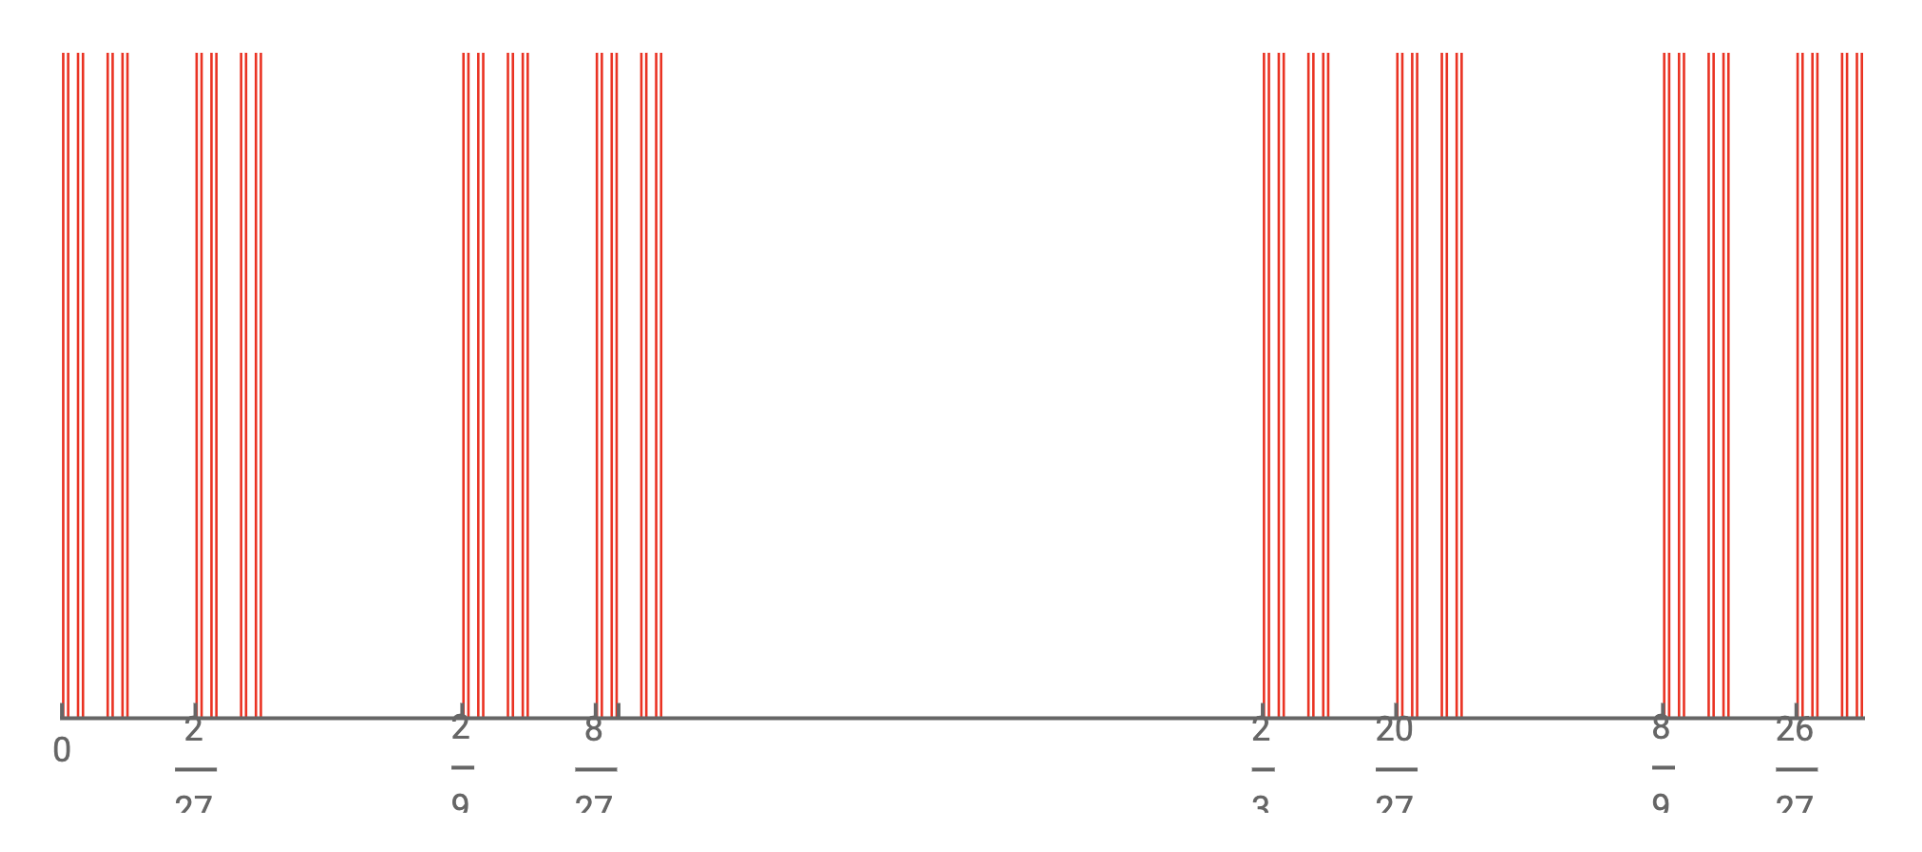
\includegraphics[width=0.6\textwidth]{images/cantor-set.png}
  \caption{Cantor Set: first few steps of construction}
  \label{fig:cantor-set}
\end{figure}

\begin{proposition}
  \begin{enumerate}
    \item $C_0$ is compact and $C_0 \subset [0,1]$;
    \item $C_0$ is nowhere dense;
    \item $\mu(C_0) = 0$
          \begin{proof}

          \end{proof}
    \item $C_0$ is continual.
          \begin{proof}

          \end{proof}
  \end{enumerate}
\end{proposition}

\begin{definition}[Fat Cantor Set]\index{Fat Cantor Set}

  A \textbf{fat Cantor set\footnote[1]{It is also sometimes called \textbf{Smith–Volterra–Cantor set (SVC)} or \textbf{$\eps$-Cantor set}.}} is an example of a set of points on the real line that is nowhere dense (in particular it contains no intervals), yet has positive measure.

  It is a generalization of the standard Cantor set $C_0$, which has measure zero.
\end{definition}

\begin{example}
  Consider $A$ be the subset of points in $[0,1]$ the decimal expansion of which doesn’t contain the digit $5$. Approximate $A$ by “first $n$ digits” sets.

  For each $n\in\mathbb{N}$ let \(A_n = \{x\in[0,1]: \text{among the first }n\text{ decimal digits of }x\text{ no digit equals }5\}.\)

  Then $A_1\supset A_2\supset\cdots$ and $A=\bigcap_{n=1}^\infty A_n$.

  Each $A_n$ is the disjoint union of $9^n$ intervals of length $10^{-n}$ (one for each choice of $n$ digits from $\{0,1,2,3,4,6,7,8,9\}$), hence \(m(A_n)=9^n\cdot10^{-n}=\Big(\frac{9}{10}\Big)^n.\)

  By continuity of measure, \(m(A)=m\Big(\bigcap_{n=1}^\infty A_n\Big)=\lim\limits_{n\to\infty}m(A_n)=\lim\limits_{n\to\infty}\Big(\frac{9}{10}\Big)^n=0.\)

  So $A$ is measurable and $m(A)=0$.
\end{example}













\subsubsection{Cantor Staircase Function}

\begin{definition}

\end{definition}

\begin{figure}[htbp]
  \centering
  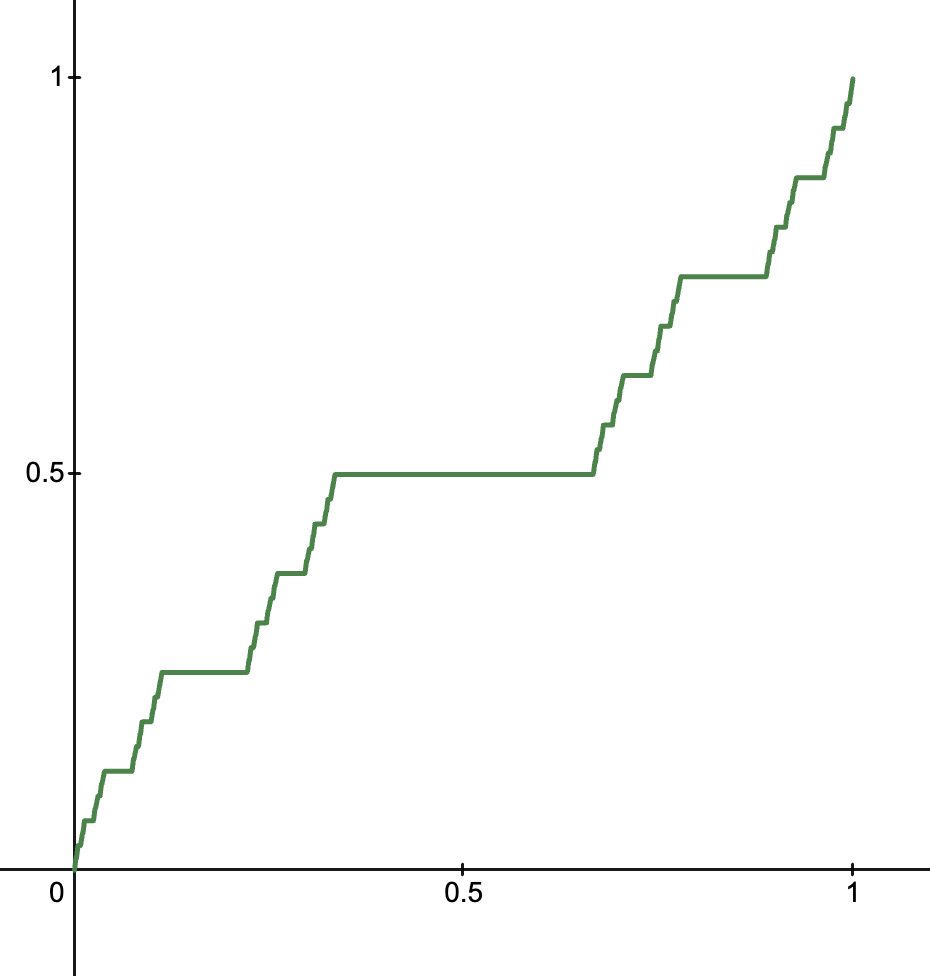
\includegraphics[width=0.45\textwidth]{images/cantor-staircase.png}
  \caption{Cantor Staircase Function}
  \label{fig:cantor-staircase}
\end{figure}

\begin{lemma}
  Let $f: \Omega \rightarrow \Omega^{\prime}, S^{\prime} \subset 2^{\Omega^{\prime}}$, then $\mathcal{A}(f^{-1}*(S^{\prime})) = f^{-1}(\mathcal{A}(S^{\prime}))$.
  \begin{proof}

  \end{proof}
\end{lemma}

\begin{corollary}
  (Preimage of Borel set is Borel.)

  If $f: [a,b] \rightarrow [c,d]$ is continuous, then $f^{-1}(E^{\prime})$ is Borel, provided $E^{\prime} \subset [c,d]$ is Borel.
  \begin{proof}
    Follows from $f^{-1}(G)$ is open if $G$ is open.
  \end{proof}
\end{corollary}


Now, consider $\phi (x) := x + K(x)$, $\phi : [0,1] \rightarrow [0,2]$, $\phi$ is strictly increasing.












\subsubsection{Construction of a Non-Borel Measurable Set(!)}
















\clearpage


\begin{proposition}
  Let $A \subset \R^n$ be a Lebesgue mesurable set, i.e. $A \in \mathcal{M}(\R^n)$.

  Then, $\forall \delta > 0$, $\exists$ a closed $F_\delta$ and an open $G_\delta$ satisfying $F_\delta \subset A \subset G_\delta$, s.t. $\mu(A \setminus F_\delta) < \delta$ and $\mu(G_\delta \setminus A) < \delta$.
  \begin{proof}

  \end{proof}
\end{proposition}

\begin{corollary}
  $\forall A \in \mathcal{M}(\R^n)$, A can be decomposed as:

  1. $A = F \bigsqcup E$, where $F$ is Borel and $E$ is measure 0;

  2. $A = G \setminus E$, where $G$ is Borel and $E \subset G$ is measure 0.
  \begin{proof}
    1. If $\mu(A) < \infty$:

    Take $F := \bigcup_{k=1}^{\infty} F_{\frac{1}{2^k}}$.

    Then $F \subset A$ and $\forall k$, $\mu(F) \geq \mu(F_{\frac{1}{2^k}}) > \mu(A) - \frac{1}{2^k}$.

    $\Rightarrow \mu(F) \geq \mu(F) \geq \mu(A)$

    $\Rightarrow \mu(F) = \mu(A)$, $\mu(A \setminus F) = 0$.

    Now, if $\mu(A) = \infty$, then we can write $A = \bigsqcup_{k=1}^{\infty} A_k$ with all $\mu(A_k) < \infty$.

    Then, $\forall A_k = F_k \bigsqcup E_k$.

    Just take $F = \bigsqcup_{k=1}^{\infty} F_k$ and $E = \bigsqcup_{k=1}^{\infty} E_k$.

    2. Proof is analogous to 1.
  \end{proof}
\end{corollary}

\begin{remark}
  Note that the actual $F$ here is an at most countable union of closed sets. And $G$ here is an at most countable intersection of open sets.
\end{remark}

\begin{remark}
  \underline{Reminder}: $\mathcal{A}(f^{-1}(S)) = f^{-1}(\mathcal{A}(S))$ for continuous $f$ $\implies f^{-1} (E)$ is Borel if $E$ is Borel.
\end{remark}

\clearpage

\subsection{Completeness and Regularity of Measures}

In previous sections, we touched upon the concept of completeness and approximation. Here we formalize these notions, which are crucial for the ``good behavior'' of a measure.

\subsubsection{Completion of a Measure Space}

We have defined a complete measure space as one where subsets of null sets are measurable. If a space is not complete, we can always ``complete'' it.

\begin{theorem}[Completion Theorem]\index{Completion Theorem}
  Let $(\Omega, \mathcal{A}, \mu)$ be a measure space. Define $\overline{\mathcal{A}}$ as the collection of sets $E \subset \Omega$ of the form $E = A \cup N$, where $A \in \mathcal{A}$ and $N$ is a subset of some $M \in \mathcal{A}$ with $\mu(M) = 0$.
  Define $\overline{\mu}(E) = \mu(A)$.
  Then:
  \begin{enumerate}
    \item $\overline{\mathcal{A}}$ is a $\sigma$-algebra.
    \item $\overline{\mu}$ is well-defined and is a measure on $\overline{\mathcal{A}}$.
    \item $\overline{\mu}$ extends $\mu$, i.e., $\overline{\mu}(A) = \mu(A)$ for all $A \in \mathcal{A}$.
    \item $(\Omega, \overline{\mathcal{A}}, \overline{\mu})$ is a complete measure space, called the \textbf{completion} of $(\Omega, \mathcal{A}, \mu)$.
  \end{enumerate}

  \begin{proof}
    \underline{1. $\sigma$-algebra:}
    Clearly $\emptyset \in \overline{\mathcal{A}}$.
    Let $E = A \cup N \in \overline{\mathcal{A}}$ with $N \subset M, \mu(M)=0$. Then $E^c = (A \cup N)^c = A^c \cap N^c$.
    Notice $A^c \cap M^c \subset E^c \subset A^c$.
    So $E^c = (A^c \cap M^c) \cup (E^c \setminus (A^c \cap M^c))$.
    The second part is a subset of $M$, hence a null subset. The first part is in $\mathcal{A}$. Thus $E^c \in \overline{\mathcal{A}}$.
    Countable union is straightforward.

    \underline{2. Well-definedness:}
    Suppose $A_1 \cup N_1 = A_2 \cup N_2$, with $N_i \subset M_i, \mu(M_i)=0$.
    We need to show $\mu(A_1) = \mu(A_2)$.
    $A_1 \subset A_2 \cup N_2 \subset A_2 \cup M_2 \implies \mu(A_1) \leq \mu(A_2) + \mu(M_2) = \mu(A_2)$.
    Symmetrically, $\mu(A_2) \leq \mu(A_1)$. Thus $\overline{\mu}$ is independent of representation.

    \underline{3. \& 4.} Follow directly from definitions. Completeness holds because if $F \subset E \in \overline{\mathcal{A}}$ and $\overline{\mu}(E)=0$, then $E = A \cup N$ where $\mu(A)=0$. $F$ is a subset of a null set, hence $F \in \overline{\mathcal{A}}$ by construction.
  \end{proof}
\end{theorem}

\subsubsection{Regularity of Measures}

Regularity connects measure theory with topology. We essentially ask: can measurable sets be approximated by open or compact sets?

\begin{definition}[Outer Regular Measure]\index{Outer Regular Measure}
  Let $X$ be a metric space (or topological space) and $\mu$ a measure on the Borel $\sigma$-algebra $\mathcal{B}(X)$.

  $\mu$ is \textbf{outer regular} on $E$ if $\mu(E) = \inf \{ \mu(U) : E \subset U, U \text{ is open} \}$.
\end{definition}

\begin{definition}[Inner Regular Measure]\index{Inner Regular Measure}
  Let $X$ be a metric space (or topological space) and $\mu$ a measure on the Borel $\sigma$-algebra $\mathcal{B}(X)$.

  $\mu$ is \textbf{inner regular} on $E$ if $\mu(E) = \sup \{ \mu(K) : K \subset E, K \text{ is compact} \}$.
\end{definition}

\begin{definition}[Regular Measure]\index{Regular Measure}
  Let $X$ be a metric space (or topological space) and $\mu$ a measure on the Borel $\sigma$-algebra $\mathcal{B}(X)$.

  $\mu$ is \textbf{regular} if it is both outer and inner regular for all sets in $\mathcal{B}(X)$.
\end{definition}

\begin{theorem}[Regularity of Lebesgue Measure]\index{Regularity of Lebesgue Measure}
  The Lebesgue measure $\mu$ on $\R^n$ is regular.
  Specifically, for any Lebesgue measurable set $E$:
  \begin{enumerate}
    \item (Outer Regularity) $\mu(E) = \inf \{ \mu(U) : E \subset U, U \text{ open} \}$.
    \item (Inner Regularity) $\mu(E) = \sup \{ \mu(K) : K \subset E, K \text{ compact} \}$.
  \end{enumerate}

  \begin{proof}
    \textbf{1. Outer Regularity:}
    This follows directly from the definition of the outer measure $\mu^*$ (covering by cells) and the fact that cells can be slightly expanded to be open.
    For $\epsilon > 0$, cover $E$ by $\{I_j\}$ such that $\sum |I_j| < \mu(E) + \epsilon/2$. Expand each $I_j$ to an open $U_j$ such that $\mu(U_j) < \mu(I_j) + \epsilon/2^{j+1}$. Then $U = \cup U_j$ is open and satisfies the condition.

    \textbf{2. Inner Regularity:}
    First, assume $E$ is bounded. By Prop 5.86, for $\epsilon > 0$, there exists a closed set $F \subset E$ such that $\mu(E \setminus F) < \epsilon$. Since $E$ is bounded, $F$ is bounded and closed, hence compact (Heine-Borel). Thus $\mu(F) > \mu(E) - \epsilon$.

    If $E$ is unbounded, define $E_k = E \cap B_k(0)$ (intersection with ball of radius $k$). Then $E_k$ is bounded and $\mu(E_k) \to \mu(E)$.
    For each $E_k$, we can find compact $K_k \subset E_k$ close in measure. By choosing $k$ large enough and then $K_k$, we obtain the result.
  \end{proof}
\end{theorem}

\clearpage

\subsection{Dynkin Classes}

In the extension of measures (Carathéodory's Theorem), we constructed a measure on a $\sigma$-algebra generated by a semi-ring. A natural question arises: Is this extension unique?
To answer this, we introduce the concept of Dynkin classes (also known as $\lambda$-systems) and $\pi$-systems. This is a powerful tool often referred to as the $\pi$-$\lambda$ Theorem.

\subsubsection{$\pi$-systems and $\lambda$-systems}

\begin{definition}[$\pi$-system]\index{$\pi$-system}
  A collection of sets $\mathcal{P} \subset 2^\Omega$ is called a \textbf{$\pi$-system} if it is closed under finite intersection:
  \[ A, B \in \mathcal{P} \implies A \cap B \in \mathcal{P}. \]
\end{definition}

\begin{example}
  The collection of all semi-open cells in $\R^n$ is a $\pi$-system.
  The collection of all open sets is a $\pi$-system.
\end{example}

\begin{definition}[$\lambda$-system / Dynkin Class]\index{$\lambda$-system}
  A collection of sets $\mathcal{D} \subset 2^\Omega$ is called a \textbf{$\lambda$-system} (or a Dynkin class) if:
  \begin{enumerate}
    \item $\Omega \in \mathcal{D}$.
    \item If $A, B \in \mathcal{D}$ and $A \subset B$, then $B \setminus A \in \mathcal{D}$ (Closed under proper difference).
    \item If $A_n \in \mathcal{D}$ and $A_1 \subset A_2 \subset \dots$, then $\bigcup_{n=1}^\infty A_n \in \mathcal{D}$ (Closed under monotone limits).
  \end{enumerate}
\end{definition}

\begin{remark}
  It is easy to check that a $\sigma$-algebra is always a $\lambda$-system and a $\pi$-system.
  Conversely, if a system is both a $\pi$-system and a $\lambda$-system, it is a $\sigma$-algebra.
  \begin{proof}
    Let $\mathcal{C}$ be $\pi$-system + $\lambda$-system.
    1. $\Omega \in \mathcal{C}$ ($\lambda$-prop).
    2. Closed under complement: $A^c = \Omega \setminus A$. Since $A \subset \Omega$, $A^c \in \mathcal{C}$ ($\lambda$-prop).
    3. Closed under union: $A \cup B = (A^c \cap B^c)^c$. Since closed under complement and intersection ($\pi$-prop), it is closed under finite union.
    4. Closed under countable union: Let $A_n \in \mathcal{C}$. Let $B_n = \bigcup_{k=1}^n A_k \in \mathcal{C}$. $B_n \subset B_{n+1}$. By $\lambda$-prop (3), $\bigcup B_n = \bigcup A_n \in \mathcal{C}$.
  \end{proof}
\end{remark}

\subsubsection{$\pi$-$\lambda$ Theorem}

\begin{theorem}[$\pi$-$\lambda$ Theorem, Dynkin]\index{$\pi$-$\lambda$ Theorem, Dynkin}
  If $\mathcal{P}$ is a $\pi$-system and $\mathcal{D}$ is a $\lambda$-system such that $\mathcal{P} \subset \mathcal{D}$, then
  \[ \sigma(\mathcal{P}) \subset \mathcal{D}, \]
  where $\sigma(\mathcal{P})$ is the smallest $\sigma$-algebra generated by $\mathcal{P}$.
\end{theorem}

\begin{proof}
  Let $\mathcal{D}(\mathcal{P})$ be the smallest $\lambda$-system containing $\mathcal{P}$ (intersection of all such $\lambda$-systems). Clearly $\mathcal{D}(\mathcal{P}) \subset \mathcal{D}$.
  It suffices to show that $\mathcal{D}(\mathcal{P})$ is a $\pi$-system. (Because if so, by the Remark above, $\mathcal{D}(\mathcal{P})$ is a $\sigma$-algebra containing $\mathcal{P}$, hence $\sigma(\mathcal{P}) \subset \mathcal{D}(\mathcal{P}) \subset \mathcal{D}$).

  \underline{Step 1}: Let $A \in \mathcal{D}(\mathcal{P})$. Define $\mathcal{D}_A = \{ B \in \mathcal{D}(\mathcal{P}) : A \cap B \in \mathcal{D}(\mathcal{P}) \}$.
  We show $\mathcal{D}_A$ is a $\lambda$-system.
  \begin{itemize}
    \item $\Omega \cap A = A \in \mathcal{D}(\mathcal{P}) \implies \Omega \in \mathcal{D}_A$.
    \item Let $B_1 \subset B_2$ in $\mathcal{D}_A$. Then $A \cap (B_2 \setminus B_1) = (A \cap B_2) \setminus (A \cap B_1)$. Since $A \cap B_1 \subset A \cap B_2$ are in $\mathcal{D}(\mathcal{P})$ and $\mathcal{D}(\mathcal{P})$ is a $\lambda$-system, the difference is in $\mathcal{D}(\mathcal{P})$. So $B_2 \setminus B_1 \in \mathcal{D}_A$.
    \item Let $B_n \uparrow B$ in $\mathcal{D}_A$. $A \cap B = \bigcup (A \cap B_n)$. By monotone limit property of $\mathcal{D}(\mathcal{P})$, $A \cap B \in \mathcal{D}(\mathcal{P})$.
  \end{itemize}

  \underline{Step 2}: Let $A \in \mathcal{P}$. Since $\mathcal{P}$ is a $\pi$-system, for any $B \in \mathcal{P}$, $A \cap B \in \mathcal{P} \subset \mathcal{D}(\mathcal{P})$. Thus $\mathcal{P} \subset \mathcal{D}_A$.
  Since $\mathcal{D}_A$ is a $\lambda$-system, we have $\mathcal{D}(\mathcal{P}) \subset \mathcal{D}_A$.
  This implies: $\forall A \in \mathcal{P}, \forall B \in \mathcal{D}(\mathcal{P}), A \cap B \in \mathcal{D}(\mathcal{P})$.

  \underline{Step 3}: Now let $B \in \mathcal{D}(\mathcal{P})$ be arbitrary (not just in $\mathcal{P}$).
  From Step 2, we know that for any $A \in \mathcal{P}$, $A \cap B \in \mathcal{D}(\mathcal{P})$.
  This means $A \in \mathcal{D}_B$. So $\mathcal{P} \subset \mathcal{D}_B$.
  Again, since $\mathcal{D}_B$ is a $\lambda$-system, $\mathcal{D}(\mathcal{P}) \subset \mathcal{D}_B$.
  This implies: $\forall B \in \mathcal{D}(\mathcal{P}), \forall C \in \mathcal{D}(\mathcal{P}), B \cap C \in \mathcal{D}(\mathcal{P})$.
  Thus $\mathcal{D}(\mathcal{P})$ is closed under intersection (a $\pi$-system). $\qed$
\end{proof}

\subsubsection{Application: Uniqueness of Measure Extension}

\begin{theorem}[Uniqueness of Measure]\index{Uniqueness of Measure}
  Let $\mu_1$ and $\mu_2$ be two measures on $(\Omega, \sigma(\mathcal{P}))$, where $\mathcal{P}$ is a $\pi$-system.
  If:
  \begin{enumerate}
    \item $\mu_1(A) = \mu_2(A)$ for all $A \in \mathcal{P}$,
    \item $\Omega = \bigcup_{n=1}^\infty E_n$ with $E_n \in \mathcal{P}$ and $\mu_1(E_n) = \mu_2(E_n) < \infty$ for all $n$ ($\sigma$-finite condition),
  \end{enumerate}
  Then $\mu_1 = \mu_2$ on $\sigma(\mathcal{P})$.
\end{theorem}

\begin{proof}
  Let's prove for the finite case ($\mu(\Omega) < \infty$) first.
  Let $\mathcal{L} = \{ E \in \sigma(\mathcal{P}) : \mu_1(E) = \mu_2(E) \}$.
  \begin{itemize}
    \item $\Omega \in \mathcal{L}$ by assumption.
    \item If $A \subset B$ are in $\mathcal{L}$, $\mu_1(B \setminus A) = \mu_1(B) - \mu_1(A) = \mu_2(B) - \mu_2(A) = \mu_2(B \setminus A)$. So $B \setminus A \in \mathcal{L}$.
    \item If $A_n \uparrow A$ are in $\mathcal{L}$, by continuity of measure, $\mu_i(A) = \lim \mu_i(A_n)$. Thus $A \in \mathcal{L}$.
  \end{itemize}
  So $\mathcal{L}$ is a $\lambda$-system containing $\mathcal{P}$. By the $\pi$-$\lambda$ Theorem, $\sigma(\mathcal{P}) \subset \mathcal{L}$.
  The $\sigma$-finite case follows by restricting measures to $E_n$ and taking limits.
\end{proof}

\begin{remark}
  This theorem is fundamental. It tells us that the Lebesgue measure we constructed is the \textbf{unique} measure on $\mathcal{B}(\R^n)$ that assigns the volume $l(I)$ to every cell $I$.
\end{remark}

\clearpage

\section{Measurable Function}

\clearpage

\subsection{What Kind of Functions are Measurable(?)}

\begin{definition}[Measurable Function]\index{Measurable Function}

  Let $(\Omega, \mathcal{A}, \mu)$ be a measure space with a complete measure. Then a function $f: \Omega \rightarrow \R$ is called \textbf{measurable} if and only if $\forall$ Borel set $A \subset \R$, it holds $f^{-1}(A) \in \mathcal{M}(\Omega)$.
\end{definition}

\begin{remark}

\end{remark}

\begin{remark}

\end{remark}

\clearpage

\subsection{Properties of Measurable Functions}

\begin{proposition}
  \begin{enumerate}
    \item If $f$ is measurable, then $a f + b$ is measurable for $a, b \in \R$;

          \noindent\medskip Define $E_c := \{x \in \Omega: af(x)+b<c\}$







    \item If $f$, $g$ are measurable, then the set $\{x: f(x)<g(x)\}$ is measurable.
          \begin{proof}

          \end{proof}

    \item Combining \textit{1} and \textit{2}, one can get:

          \ldots

          $\Rightarrow f \pm g$ is measurable.

    \item If $\phi \in \mathcal{C}(\R)$ and $f$ is measurable, then $\phi \circ f$ is measurable.
          \begin{proof}

          \end{proof}

          \begin{remark}

          \end{remark}

    \item If $f,g$ are measurable, then $f \cdot g$ is measurable.
          \begin{proof}

          \end{proof}

    \item If $f,g$ are measurable and $g(x) \neq 0, \forall x \in \Omega$, then $\frac{f}{g}$ is measurable.
          \begin{proof}
            $f \div g = f \cdot \frac{1}{g}$ with $\frac{1}{g}$ being measurable by taking $\phi (x) = \frac{1}{x}$ in \textit{4}.
          \end{proof}
  \end{enumerate}
\end{proposition}

\begin{remark}
  \underline{Conclusion}: Arithmetric operations with measurable functions give measurable functions.
\end{remark}



















% TODO: 只要你把函数限制在一个 Lebesgue 零测集上，这个受限函数总是 Lebesgue 可测.








\clearpage

\subsection{Almost Everywhere Properties}

\begin{definition}[Almost Everywhere]\index{Almost Everywhere}

  Let $(\Omega, \mathcal{A}, \mu)$ be a measure space with a complete measure.

  Then we say that a property of some points $\{x\ \in \Omega\}$ holds \textbf{almost everywhere (a.e.)} if and only if the property holds that $\forall x \in \Omega \setminus E$, where $\mu(E) = 0$.

  We say that a property of some points $\{x\ \in \Omega\}$ holds \textbf{almost everywhere (a.e.) on A}, where $A \in \mathcal{M}(\Omega)$, if and only if the property holds for $\forall x \in A \setminus E$, where $\mu(E) = 0$.
\end{definition}

\begin{example}
  \begin{enumerate}
    \item Dirichlet function: $D(x) = \begin{cases} 1, & x \in \Q, \\ 0, & x \in [0,1] \setminus \Q. \end{cases}$

          One can esaily check that
    \item One can consider \textbf{convergence a.e.}: $f_n(x) \rightarrow f(x)$ a.e.

    \item One can consider funtions defined a.e.:

    \item Finally,instead of actual functions, we may consider their equivalent classes:

  \end{enumerate}
\end{example}

\begin{lemma}
  If $f$ is measurable and $\mu(A) = 0$,

  then if we define:
  $g(x) = \begin{cases} f(x), & x \in A, \\ 0,  & x \notin A.\end{cases}$, $g$ is still measurable.
  \begin{proof}

  \end{proof}
\end{lemma}

\begin{theorem}
  Let $\{f_n\}_{n=1}^{\infty}$ be a sequence of measurable fucntions on $(\Omega, \mathcal{A}, \mu)$ and $f_n(x) \overset{a.e.}{\rightarrow} f(x)$. Then $f(x)$ is also measurable.
  \begin{proof}

  \end{proof}
\end{theorem}

\begin{corollary}
  Let $\{f_n(x)\}$ be a sequence of measurable functions. If $f_n(x)$ is bounded from above $\forall n$ for a.e. $x \in \Omega$, then

  \begin{enumerate}
    \item $\sup\limits_{n} f_n(x)$\ is measurable;
    \item $\limsup\limits_{n \to \infty} f_n(x)$ is measurable;
  \end{enumerate}

  If, otherwise, $f_n(x)$ is bounded from below $\forall n$ for a.e. $x \in \Omega$, then
  \begin{enumerate}
    \item $\inf\limits_{n} f_n(x)$ is measurable;
    \item $\liminf\limits_{n \to \infty} f_n(x)$ is measurable.
  \end{enumerate}

  \begin{proof}
    Consider $g_1(x) := f_1(x)$, $g_2(x) := \max\{f_1(x), f_2(x)\} = \frac{|f_1(x) - f_2(x)| + f_1(x) + f_2(x)}{2}$, $g_3(x) := \max\{f_1(x), f_2(x), f_3(x)\} = \max\{g_2(x), f_3(x)\}$, \ldots, which are all measurable by properties in the last subsubsection.

    Then, $\sup\limits_{n} f_n(x) \overset{a.e.}{=} \lim\limits_{n \to \infty} g_n(x)$ is measurable.

    \underline{Recall}: $\limsup\limits_{n \to \infty} a_n(x) = \sup \{$limits of convergent subsequences$\} = \lim\limits_{k \to \infty} (\sup\limits_{n \geq k} a_n(x))$.

    Then, $\limsup\limits_{n \to \infty} f_n(x) = \lim\limits_{k \to \infty} (\sup\limits_{n \geq k} f_n(x))$ is measurable.

    Analogously, $\inf\limits_{n} f_n(x) = - \sup\limits_{n} (-f_n(x))$ is measurable; $\liminf\limits_{n \to \infty} f_n(x) = - \limsup\limits_{n \to \infty} (-f_n(x))$ is measurable.
  \end{proof}
\end{corollary}

\clearpage

\subsection{Egorov's Theorem}

\begin{theorem}[Egorov's Theorem]\index{Egorov's Theorem}

  Let $(\Omega, \mathcal{A}, \mu)$ be a space with a \underline{finite} complete measure, and $\{f_n\}$ is a sequence of measurable functions with $f_n \overset{a.e.}{\rightarrow} f$.

  Then, $\forall \delta > 0$, $\exists$ a set $E_\delta \subset \Omega$ s.t. $\mu(E_\delta) < \delta$ and $f_n \overset{\Omega \setminus E_\delta}{\rightrightarrows} f$.

  \begin{proof}
    Fix $\delta > 0$. Consider the divergence set $E$ ($\mu(E) = 0$ by our assumption):

    $E = \bigcup_{k \geq 1} $
  \end{proof}
\end{theorem}

\begin{remark}
  Intuition here: on a set with small measure, convergence may be bad; but on the rest part with large measure, convergence is uniform.
\end{remark}

\begin{remark}
  Ths Egorov's Theorem may fail if $\mu(\Omega) = \infty$.

  \underline{Counter example 1}: Take $\Omega = \R$ with Lebesgue measure, $f_n(x) = \frac{x}{n}$.

  Then, $f_n(x) \overset{a.e.}{\rightarrow} 0$ on the whole real line, but $\forall E_\delta$ with finite measure, $f_n \not \rightrightarrows 0$ on $\R \setminus E_\delta$.

  \underline{Counter example 2}: Take $\Omega = \R$ with Lebesgue measure, $f_n(x) = \chi_{[n, n+1]}(x)$.

  Then, $f_n(x) \overset{a.e.}{\rightarrow} 0$ on the whole real line, but $\forall E_\delta$ with finite measure, $f_n \not \rightrightarrows 0$ on $\R \setminus E_\delta$.
\end{remark}

\begin{remark}
  In Egorov's Theorem, one CANNOT take $E_\delta = 0$.

  \underline{Counter example}: Take $\Omega = [0,1]$ with Lebesgue measure, $f_n(x) = x^n$.

  Then, $f_n(x) \overset{a.e.}{\rightarrow} 0$ for $x \in [0,1)$ and $f(1) = 1$.
\end{remark}

\begin{proposition}
  Let $E \subset \R$ be a closed set, $f \in \mathcal{C}(E)$. Then $\exists g \in \mathcal{C}(\R)$, s.t. $g|_E = f|_E$.
  \begin{proof}
    Since $E$ is closed, $\R \setminus E$ is open. So, we can write $\R \setminus E = \bigsqcup_{k=1}^{\infty} I_k$, where $I_k = (a_k, b_k)$.

    On each $I_k$, we define $g$ as the linear function connecting $(a_k, f(a_k))$ and $(b_k, f(b_k))$. Explicitly, $g(x) = f(a_k) + \frac{f(b_k) - f(a_k)}{b_k - a_k}(x - a_k), x \in I_k$.

    If there are some intervals which contain $\infty$ or $-\infty$, we just extend $g$ as a constant function on them.

    So, such defined $g$ is continuous on $\R$ and $g|_E = f|_E$.
  \end{proof}
\end{proposition}

\begin{remark}
  What's good about such linear link / extension?

  Linear functions not only preserves continuity, but also linear control, which may provide us with some sort of convenience in some problems.
\end{remark}

\begin{remark}
  This also works for $E \subset \R^n$, which requires a more complicated proof.
\end{remark}






\clearpage

\subsection{Lusin's Theorem}

\begin{theorem}[Lusin's Theorem]\index{Lusin's Theorem}

  Let $f$ be a Lebesgue measurable function on $[a,b]$.

  Then $\forall \delta > 0$, $\exists E_\delta$ s.t. $\mu(E_\delta) < \delta$ and $\exists$ a continuous function $g \in \mathcal{C}([a,b])$, s.t. $f|_{[a,b] \setminus E} = g|_{[a,b] \setminus E}$.

  \begin{proof}

  \end{proof}
\end{theorem}

\begin{remark}
  $[a,b]$ can be replaced by any interval $I \subset \R$.
\end{remark}

\begin{remark}
  We could say instead of $f|_{[a,b] \setminus E} = g|_{[a,b] \setminus E}$ that $f$ is continuous on $[a,b] \setminus E$ for an open set $E$ (as follows from the proof).
\end{remark}

\begin{remark}
  The Lusin's Theorem also holds in $\R^n$ analogously: for $f$ - measurable on an open $G \subset \R^n$.
\end{remark}

\begin{remark}
  We still CANNOT take $E$ with $\mu(E) = 0$.

  \underline{Counter Example}: $f(x) = \begin{cases} \frac{1}{x}, & x \in (0,1]; \\ 0, & x = 0 \end{cases}$
\end{remark}

\begin{theorem}[Inverse Lusin's Theorem]\index{Inverse Lusin's Theorem}

  Let $f$ be a function on $[a,b]$ with the \textbf{Lusin property} ($\forall \delta > 0$, $\exists E_\delta : \mu(E_\delta) < \delta$ and $g_\delta \in \mathcal{C}([a,b]): f|_{[a,b] \setminus E} = g|_{[a,b] \setminus E}$).

  Then $f$ is Lebesgue measurable.

  So, $f$ on $[a,b]$ is Lebesgue measurable $\Leftrightarrow$ $f$ has the Lusin property.
  \begin{proof}



  \end{proof}
\end{theorem}


We established, in particular, that a measurable function on an interval is an a.e. limit of continuous functions.


\clearpage

\subsection{Convergence in Measure}

\begin{definition}[Convergence in Measure]\index{Convergence in Measure}

  Let $f_n$ be a sequence of measurable functions on a measure space $(\Omega, \mathcal{A}, \mu)$ with a complete measure. We say that $f_n$ \textbf{converges to $f$ in measure} if $\forall \delta > 0$,
  $$\lim_{n \to \infty} \mu(\{x \in \Omega \colon |f_n(x) - f(x)| \geq \delta\}) = 0.$$

  In the theory of probability, this is also called \textbf{convergence in probability}.

  \underline{Notation}: $X_n \xrightarrow{p} X$ where $X_n, X$ are all random variables.
\end{definition}

\begin{theorem}
  Let $(\Omega, \mathcal{A}, \mu)$ be a space with a \underline{finite} complete measure. $f_n \overset{a.e.}{\rightarrow} f$ where $f_n$ is measurable.

  Then $f_n \rightarrow f$ in measure.
  \begin{proof}
    $f_n \overset{a.e.}{\rightarrow} f$ on $\Omega$. Fix $\delta > 0$, then fix $\eps > 0$.

    By Egorov's Theorem, $\exists E: \mu(E) < \eps$ and $f_n \overset{\Omega \setminus E}{\rightrightarrows} f$. Then, $\exists N \in \N, \forall n > N, |f_n(x) - f(x)| < \delta$ on $\Omega \setminus E \Rightarrow \{\}$









  \end{proof}
\end{theorem}

\begin{remark}

\end{remark}


\begin{theorem}[Riesz Theorem]\index{Riesz Theorem}

  Let $(\Omega, \mathcal{A}, \mu)$ be a space with a \underline{finite} complete measure. $f_n \rightarrow f$ in measure.

  Then,$\exists f_{n_k} \overset{a.e.}{\rightarrow} f (k \rightarrow \infty)$ on $\Omega$.
  \begin{proof}
    Fix $k \in \N$, then $\mu(\{|f_n - f| > \frac{1}{k}\}) \overset{n \rightarrow \infty}{\rightarrow} 0$.

    $\Rightarrow \exists n_k: \mu(\{|f_{n_k}(x) - f(x)| \geq \frac{1}{k}\}) < \frac{1}{2^k}$.

    Denote $E_k := \{|f_{n_k}(x) - f(x)| \geq \frac{1}{k}\}$, then $\mu(E_k) < \frac{1}{2^k}$.

    Now, set $E := \bigcap_{N=1}^{\infty} \bigcup_{k \geq N} E_k$. Denote $A_N := \bigcup_{k \geq N} E_k$.

    Then, $\mu(A_N) \leq \Sigma_{k \geq N} \mu(E_k) < \Sigma_{k \geq N} \frac{1}{2^k} = 2^{-N}$.

    But $A_1 \supset A_2 \supset \ldots$ and $\mu(A_1) < \frac{1}{2}$ (in particular, $\mu(A_1) < \infty$)

    $\Rightarrow$ we can apply the continuity of $\mu$:

    $\mu(E) = \lim\limits_{N \rightarrow \infty} \mu(A_N) = 0$.

    We can apply the continuity of $\mu$: $\mu(\bigcap_{N=1}^\infty \bigcup_{k=N}^\infty A_k) = 0$

    We claim then $f_{n_k} \to f$ a.e. $\forall x \in \Omega \setminus E$

    Indeed, $\mu(\limsup E_k) = \mu(\bigcap_{N=1}^\infty \bigcup_{k=N}^\infty \{|f_{n_k} - f| \ge \frac{1}{k}\}) = 0$.

    If $x \in \Omega \setminus E$, then $\exists N$: for $k \ge N$, it holds $|f_{n_k}(x) - f(x)| < \frac{1}{k}$ in partic.

    $f_{n_k}(x) \to f(x)$, as desired.
  \end{proof}
\end{theorem}

\begin{example}
  $\Omega = [0, 1)$, now let's build a sequence of intervals.
  \begin{align*}
    A_1 & = [0, 1),                                               \\
    A_2 & = [0, 1/2), & A_3   & = [1/2, 1)                        \\
    A_4 & = [0, 1/3), & A_5   & = [1/3, 2/3), & A_6 & = [2/3, 1), \\
    A_7 & = [0, 1/4), & \dots
  \end{align*}

  Let $f_n(x) = \mathds{1}_{A_n}(x) := \begin{cases} 1, & x \in A_n \\ 0, & x \notin A_n \end{cases}$

  \begin{center}
    \begin{tikzpicture}[scale=1.5, >=Stealth]

      \begin{scope}[shift={(0, 0)}]
        \draw[->] (0, 0) -- (1.2, 0) node[right] {$x$};
        \draw[->] (0, 0) -- (0, 1.2) node[above] {$f_1$};
        \draw[thick, red] (0, 1) -- (1, 1);
        \filldraw[red] (0, 1) circle (0.02); % Closed dot at 0
        \draw (1, 1) circle (0.02); % Open dot at 1 (since [0, 1))
        \node at (1, -0.2) {$1$};
      \end{scope}

      \begin{scope}[shift={(2.5, 0)}]
        \draw[->] (0, 0) -- (1.2, 0) node[right] {$x$};
        \draw[->] (0, 0) -- (0, 1.2) node[above] {$f_2$};
        \draw[thick, red] (0, 1) -- (0.5, 1);
        \draw[thick] (0.5, 0) -- (1, 0);
        \filldraw[red] (0, 1) circle (0.02);
        \draw (0.5, 1) circle (0.02);
        \node at (0.5, -0.2) {$\frac{1}{2}$};
        \draw (0.5, 0.05) -- (0.5, -0.05); % Tick mark at 1/2
        \node at (1, -0.2) {$1$};
        \draw (1, 0.05) -- (1, -0.05); % Tick mark at 1
      \end{scope}

      \begin{scope}[shift={(5, 0)}]
        \draw[->] (0, 0) -- (1.2, 0) node[right] {$x$};
        \draw[->] (0, 0) -- (0, 1.2) node[above] {$f_3$};
        \draw[thick, red] (0.5, 1) -- (1, 1);
        \draw[thick] (0, 0) -- (0.5, 0);
        \filldraw[red] (0.5, 1) circle (0.02);
        \draw (1, 1) circle (0.02);
        \node at (0.5, -0.2) {$\frac{1}{2}$};
        \draw (0.5, 0.05) -- (0.5, -0.05); % Tick mark at 1/2
        \node at (1, -0.2) {$1$};
        \draw (1, 0.05) -- (1, -0.05); % Tick mark at 1
      \end{scope}

      \begin{scope}[shift={(7.5, 0)}]
        \draw[->] (0, 0) -- (1.2, 0) node[right] {$x$};
        \draw[->] (0, 0) -- (0, 1.2) node[above] {$f_4$};
        \draw[thick, red] (0, 1) -- (1/3, 1);
        \draw[thick] (1/3, 0) -- (1, 0);
        \filldraw[red] (0, 1) circle (0.02);
        \draw (1/3, 1) circle (0.02);
        \node at (1/3, -0.2) {$\frac{1}{3}$};
        \draw (1/3, 0.05) -- (1/3, -0.05); % Tick mark at 1/3
        \node at (1, -0.2) {$1$};
        \draw (1, 0.05) -- (1, -0.05); % Tick mark at 1
      \end{scope}

      \begin{scope}[shift={(9, 0)}]
        \node at (0.6, 0.6) {etc.};
      \end{scope}
    \end{tikzpicture}
  \end{center}

  Then, for example, for $x \in [0, 1)$, $x$ will fall into infinitely many of $A_n \implies$ $f_n(x) = 1$ and $x \in A_m$ for infinitely many of $m$, so $f_m(x) = 0$

  Thus, $\not\exists \lim_{n \to \infty} f_n(x)$ $\forall x \in [0, 1)$.

  But $\mathds{1}_{[0,\frac{1}{k}]}(x) \overset{k \to \infty}{\rightarrow} 0$ a.e. and $\mathds{1}_{[0,\frac{1}{k}]}$ is a subset of $f_n$.
\end{example}

\clearpage

\section{Lebesgue Integration with a Finite Complete Measure}

The Riemann integral relies on a geometric partitioning of the domain, which fails when the function exhibits rapid local oscillation (making approximation by vertical rectangles impossible). In contrast, the Lebesgue integral adopts a statistical perspective by partitioning the range. It aggregates the measure of sets where the function takes specific values, thereby handling such irregularities robustly.

\vspace{1cm}

\noindent In what follows: $(\Omega, \mathcal{A}, \mu)$ --- a space with \underline{finite} complete measure.

\noindent ($\Omega$: set, $\mathcal{A}$: $\sigma$-algebra on $\Omega$, $\mu$: $\sigma$-additive measure on $\mathcal{A}$.)

\noindent Define the extended real number set $\overline{\mathbb{R}} = \mathbb{R} \cup \{-\infty, +\infty\}$ and we have the axiom: $0 \cdot \infty = 0$.

\clearpage

\subsection{Simple Function}

\begin{definition}[Simple Function]\index{Simple Function}

  A function $f$ on $\Omega$ is \textbf{simple}, if $f(\Omega)$ is at most countable, i.e. $f(\Omega) = \{c_j\}_{j=1}^\infty$.
\end{definition}

\begin{lemma}
  A simple $f$ is measurable $\iff$ all the 'level sets\footnote[1]{We also call them canonical sets because they are the canonical objectives we analyzes here.}' $E_j = \{x \in \Omega \colon F(x) = c_j\}$ are measurable.
\end{lemma}

\begin{theorem}
  $f$ is measurable on $\Omega$ $\iff$ $f$ can be expressed as a uniform convergence of a sequence of simple measurable functions on $\Omega$, i.e. $\exists f_n \overset{\Omega}{\rightrightarrows} f$ where all $f_n$ are simple and measurable.
  \begin{proof}
    1. Suppose $f$ can be expressed as an uniformly convergence of some sequence of simple measurable functions, then f is clearly measurable. (Recall that we have a theorem saying that the a.e. convergence of a sequence of mesurable functions is still measurable.)

    2. Suppose $f$ is measurable on $\Omega$

    Fix $n \in \N$, then $\R = \bigsqcup_{k = -\infty}^{+\infty} [\frac{k-1}{2^n}, \frac{k}{2^n})$.

    Let $E_n^k = f^{-1}([\frac{k-1}{2^n}, \frac{k}{2^n}))$. $\forall E_n^k, \forall x \in E_n^k$, we set $f_n(x) = \frac{k-1}{2^n}$.

    Then, $\Omega = \bigsqcup_{k = -\infty}^{+\infty} E_n^k, f_n|_{E_n^k} = \frac{k-1}{2^n}$. $f_n$ is well-defined on $\Omega$.

    Since $f$ is measurable, all $E_n^k$ are measurable $\Rightarrow$ $f_n$ is measurable.

    Clearly, $|f_n(x) - f(x)| \leq \frac{1}{2^n} \Rightarrow f_n \overset{\Omega}{\rightrightarrows} f$.
  \end{proof}
\end{theorem}

\begin{remark}
  Here, clearly it could be possible that $f$ takes its value as $\infty$ on some measure-zero set, which requires us to deal with the construction more carefully. For this specific construction, we define $\forall x \in E_{\infty}, f_n(x) = f(x)$. Such construction has no problem since $E_\infty$ has measure zero and still $|f_n(x) - f(x)| \leq \frac{1}{2^n}$.
\end{remark}

\begin{remark}
  As seen from the proof, we may, in addition:

  \begin{enumerate}
    \item make $f_n \rightrightarrows f$ where all $f_n$ are \underline{non-decreasing} in $n$, just as in the proof;
          \begin{proof}
            At step $n$, $f_n$ approximates $f$ using intervals of size $1/2^n$.

            At step $n+1$, we split those intervals in half to get better precision. Because we are taking the "floor" (the lower bound of the interval $\frac{k-1}{2^n}$), refining the grid moves the approximation up or keeps it the same; it never moves it down.
          \end{proof}
    \item make $f_n \rightrightarrows f$ where all $f_n$ are \underline{non-increasing} in $n$, by setting $f_n(x) = \frac{k}{2^n}$;
    \item $f \geq 0 \Rightarrow$ choose $f_n \geq 0$, just as in the proof (since $f \geq 0$, $E_n^k = \emptyset$, $\forall k < 0$);
    \item $f$ is bounded, then choose $\{f_n\}$ which are finitely valued (need a bit modifying of the proof).
  \end{enumerate}
\end{remark}

\begin{definition}[Lebesgue Integrable Simple Function]\index{Lebesgue Integrable Simple Function}

  Let $f$ be a measurable simple function. Then we say that $f$ is \textbf{Lebesgue integrable on $\Omega$} if the series $\sum_{j=1}^{\infty}c_j \mu(E_j)$ is absolutely convergent.

  Here, $f(\Omega) = \{c_j\}_{j=1}^\infty, E_j = f^{-1}(\{c_j\})$.

  If the condition is satisfied, we call $\int_{\Omega} f d\mu := \sum_{j=1}^{\infty}c_j \mu(E_j)$ the \textbf{Lebesgue integration} of $f$ over $\Omega$.
\end{definition}

\begin{remark}
  It's convenient to write $f(x) = \sum_{j=1}^{\infty} c_j \mathds{1}_{E_j}$.
\end{remark}

\begin{remark}
  Analogously, we can define the integrability of $f$ on $A \in \mathcal{A}$ and $\int_{A} f d\mu$ $\forall A \in \mathcal{A}$.

  (Switch here to $\mathcal{A}^{\prime} := \mathcal{A} \bigcap A, \mu^{\prime}(X) := \mu(X \bigcap A)$.)
\end{remark}

\begin{remark}
  In this definition, one can actually consider any partition $\Omega = \bigsqcup_j A_j, A_j \in \mathcal{A}, f|_{A_j} = a_j \in \R, \int_{\Omega} f d\mu = \sum_{j=1}^{\infty}a_j \mu(A_j)$.

  In other words, one can easily check that our definition for Lebesgue integrable simple functions is well-defined in the sense that we only need to make sure on every $E_j$ $f$ only takes one constant value $c_j$ without requring all $c_j$ here to be precisely distinct, which is presented in the next lemma.

  So, thanks to the well-defineness of our definition for Lebesgue integration for simple functions, we can simply always choose $\{E_j\}$ as our partition for convenience, which is the 'maximum' partition.
\end{remark}

\begin{lemma}
  Let $A = \bigcup_k B_k$, where $B_i \cap B_j = \varnothing$ when $i \neq j$, and assume that the function $f$ takes a constant value $b_k$ on each set $B_k$ (We don't require them to be all distinct!). Then $\int_A f d\mu = \sum_k b_k \mu(B_k)$, and $f$ is Lebesgue integrable on $A$ if and only if the series $\sum_k b_k \mu(B_k)$ is absolutely convergent.
  \begin{proof}
    It is easy to see that each canonical set
    \(E_j = \{ x \in A : f(x) = c_j \}\)
    is the union of those sets $B_k$ satisfying $b_k = c_j$.

    Therefore,
    \(\sum_j c_j \mu(E_j) = \sum_j c_j \sum_{k: b_k = c_j} \mu(B_k) = \sum_k b_k \mu(B_k).\)

    Since the measure is non-negative, we have
    \(\sum_j |c_j| \mu(E_j) = \sum_j |c_j| \sum_{k: b_k = c_j} \mu(B_k) = \sum_k |b_k| \mu(B_k).\)

    That is, the series $\sum c_j \mu(E_j)$ and $\sum b_k \mu(B_k)$ either both converge absolutely or both diverge. The lemma is proved.
  \end{proof}
\end{lemma}

\begin{proposition}
  \begin{enumerate}
    \item Linearity: $f,g$: simple, Lebesgue integrable $\Rightarrow$ $\alpha f + \beta g$: also Lebesgue integrable $\forall \alpha, \beta \in \R$ and $\int_A (\alpha f + \beta g) d\mu = \alpha \int_A f d\mu + \beta \int_A g d\mu$.
          \begin{proof}
            $f(A) = \{c_j\}_{j=1}^{\infty}, g(A) = \{d_j\}_{j=1}^{\infty}$. $E_j := f^{-1}(c_j), G_j:= g^{-1}(d_j)$.

            $\Rightarrow \alpha f + \beta g |_{E_j \bigcap G_k} = \alpha c_j + \beta d_k$ (Note that $\{E_j \bigcap G_k\}_{j,k}$ itself makes a partition of the whole space $\Omega$.)

            $\Rightarrow$ we shall consider, for the integrability, the series

            $\sum_{j,k}(\alpha c_j + \beta d_j) \mu(E_j \bigcap G_k)$

            $=$ \{linearity of series\} $= \alpha \sum_{j,k} c_j \mu(E_j \bigcap G_k) + \beta \sum_{j,k} \mu(E_j \bigcap G_k)= $ \{$\sigma$-additivity\} = $\alpha \sum_{j} c_j \mu(E_j) + \beta \sum_{k} d_k \mu(G_k)$ where the last two series are absolutely convergent. Thus, the original series is absolutely convergent.

            Also, we have $\int_A (\alpha f + \beta g) d\mu = \alpha \int_A f d\mu + \beta \int_A g d\mu$ by definition.
          \end{proof}
    \item If $f$ is a \underline{bounded} simple function: $|f| \leq C$ for some $C \in \R^+$ $\implies$ $f$ is Lebesgue integrable and $|\int_A f d\mu| \leq C \mu(A)$.
          \begin{proof}
            $\sum |c_j \mu(E_j)| \leq C \sum \mu(E_j) = C \mu(A)$

            $\implies \sum c_j \mu(E_j)$ is absolutely convergent.
          \end{proof}
  \end{enumerate}
\end{proposition}

\clearpage

\subsection{Lebesgue Integral with a Finite Complete Measure}

The Lebesgue integral is less concerned with the function's behavior at individual points; rather, it focuses on the measure of the sets where the function assumes specific values.

\begin{definition}[Lebesgue Integrable Function]\index{Lebesgue Integrable Function}

  Let $f$ be a general measurable function on $(\Omega, \mathcal{A}, \mu)$.

  Then $f$ is called \textbf{Lebesgue integrable} on $A \subset \mathcal{A}$ if $\exists$ a sequence of simple, measurable, Lebesgue integrable (on $A$) functions $\{f_n\}$ s.t. $f_n \overset{A}{\rightrightarrows} f$.

  \underline{Notation}: We write $f \in \mathcal{L}^1(A)$ if $f$ is Lebesgue integrable on $A$.\footnote[1]{Here, $\mathcal{L}^1$ means $\mathcal{L}^1$-space. In general, for $1 \leq p \leq \infty$, $\mathcal{L}^p$-space is defined as the space of Lebesgue measurable functions for which the $p$-th power of the absolute value is Lebesgue integrable.}

  Further, $\int_A f d \mu := \lim\limits_{n \rightarrow \infty} \int_A f_n d \mu$ in the case of integrability is the \textbf{Lebesgue integration} of $f$ on $A$.
\end{definition}

\begin{proposition}
  \begin{enumerate}
    \item The limit $\lim\limits_{n \rightarrow \infty} \int_A f_n d \mu$ always exists, if $f$ is Lebesgue integrable and $f_n \overset{A}{\rightrightarrows} f$;
          \begin{proof}
            $f_n \overset{A}{\rightrightarrows} f \implies \forall \eps > 0, \exists N \in \N; \forall m, n > N, |f_n - f_m| < \eps$ on $A$.

            $\implies |\int_A f_n d\mu - \int_A f_m d\mu| =$ \{linearity of Lebesgue integration of Lebesgue integrable simple function\} = $|\int_A (f_n - f_m) d\mu| \leq \eps \mu(A)$. (Thanks to the fact that $\mu(A) < \infty$.)
          \end{proof}
    \item The value $\lim\limits_{n \rightarrow \infty} \int_A f_n d \mu$ doesn't depend on the sequence $\{f_n\}$;
          \begin{proof}
            Assume, to the contrary, that
            $L:=\lim_{n\to\infty}\int_A f_n\,d\mu$ and $L^*:=\lim_{n\to\infty}\int_A f_n^*\,d\mu$ but $L\neq L^*$.

            Construct a new sequence $\{g_n\}$ by \underline{interleaving the two sequences}:

            \(
            g_{2n-1}:=f_n, g_{2n}:=f_n^*, n=1,2,\ldots
            \)

            Since $f_n \overset{A}{\rightrightarrows} f$ and $f_n^* \overset{A}{\rightrightarrows} f$, the interleaved sequence $g_n$ also satisfies $g_n \overset{A}{\rightrightarrows} f$ (uniform convergence on $A$ is preserved under interleaving). Hence the limit
            \(
            \lim_{n\to\infty}\int_A g_n\,d\mu
            \)
            exists.

            However, the subsequence of odd indices of $\{\int_A g_n\,d\mu\}$ is exactly $\{\int_A f_n\,d\mu\}$ and therefore has limit $L$, while the subsequence of even indices is $\{\int_A f_n^*\,d\mu\}$ and has limit $L^*$. This contradicts $L\neq L^*$. Therefore $L=L^*$, and the limit is independent of the chosen approximating sequence.
          \end{proof}
    \item For simple $f$, the definition is equivalent the previous definition of 'Lebesgue integrable' for simple functios.
  \end{enumerate}
\end{proposition}

We now grab the theorem below without proving it.

\begin{theorem}[Cauthy Theorem on Permutations]\index{Cauthy Theorem on Permutations}

  Let $\sum_n a_n$ be an absolutly convergent number series.

  Then $\forall$ permutation $\delta: \N \leftrightarrow \N$, $\sum_n a_{\delta(n)}$ is also an absolutely convergent series which converges to the same sum value.
\end{theorem}

You may be more familiar with its appearance as the \textit{Riemann Rearrangement Theorom}: "If $\sum_{n=1}^{\infty} a_n$ converges absolutely, then every rearrangement of $\sum_{n=1}^{\infty} a_n$ converges, and they all converge to the same sum."

\begin{corollary}
  Let $\{a_{1n}\}_{n=1}^{\infty}$ absolutely converge to $b_1$,
  $\{a_{2n}\}_{n=1}^{\infty}$ absolutely converge to $b_2$, $\ldots$. If $\sum_i^{\infty} b_i$ absolutely converges to $b \in \R$, then $\sum_{i,j} a_{ij}$ absolutely converges to $b$.
\end{corollary}

\begin{proposition}
  \begin{enumerate}
    \item Let $f$ be a Lebesgue integrable simple function: $f(x) = \sum_{j=1}^{\infty} c_j \mathds{1}_{E_j}$, then its integration over $A$ equals $\sum_j c_j \mu(E_j)$.

          In particular, if $f = C = constant$, then $\int_A f d \mu = C \mu(A)$;

          $\qquad \qquad \qquad$ Also, $\int_A \mathds{1}_{E} d\mu = \mu(E), \forall E \subset A$.

    \item Linearity: $f,g \in \mathcal{L}^1(A) \Rightarrow$ $\alpha f + \beta g \in \mathcal{L}^1(A), \forall \alpha, \beta \in \R$ and $\int_A (\alpha f + \beta g) d\mu = \alpha \int_A f d\mu + \beta \int_A g d\mu$.
          \begin{proof}
            $\exists f_n \overset{A}{\rightrightarrows} f, g_n \overset{A}{\rightrightarrows} g$ where $\forall f_n,g_n \in \mathcal{L}^1(A)$ $\implies \alpha f_n + \beta g_n \overset{A}{\rightrightarrows} \alpha f + \beta g$,
            and by linearity of Lebesgue integrability of simple functions we get $\forall \alpha f_n + \beta g_n \in \mathcal{L}^1(A)$, where $\forall \alpha f_n + \beta g_n$ is clearly still simple, $\implies$ $\alpha f + \beta g \in \mathcal{L}^1(A)$, $\int_A (\alpha f_n + \beta g_n) d\mu$ exists and equals $\alpha \int_A f_n d\mu + \beta \int_A g_n d\mu$ by linearity of series. Taking limit $n \to \infty$, we obtain $\int_A (\alpha f + \beta g) d\mu = \alpha \int_A f d\mu + \beta \int_A g d\mu$.
          \end{proof}

    \item If $\mu(A) = 0 \implies \forall f \in \mathcal{L}^1(A)$ and $\int_A f d\mu = 0$.
          \begin{proof}
            $\forall f$: Simply use the standard\footnote[1]{Here, 'stantard' means being the same as the construction of such $\{f_n\}$ in the proof of Theorem 6.1.} $f_n \overset{A}{\rightrightarrows} f $. It's trivial that $\forall f_n \in \mathcal{L}^1(A) \implies f \in \mathcal{L}^1(A)$. Since $\mu(A) = 0$, we have $\mu(E) = 0, \forall E \subset A \implies$ by definition, $\int_A f_n d\mu = 0 \implies \int_A f d\mu = 0$.
          \end{proof}

    \item If $f = 0$ a.e. on $A$, then $f \in \mathcal{L}^1(A)$ and $\int_A f d\mu = 0$.

          As a corollary, if $f,g$ are measurable on $A$ and $f = g$ a.e. on $A$, then $f,g$ are Lebesgue integrable or not Lebesgue integrable simultaneously, and if they are Lebesgue integrable, $\int_A f d\mu = \int_A g d\mu$.

          (So, 'Lebesgue integrable' ignores measure-zero sets.)
          \begin{proof}
            Let $f = 0$ a.e. on $A$. Choose the 'standard' $f_n \overset{A}{\rightrightarrows} f$. By construction, $\forall f_n$, which is a simple function, $f_n = 0$ a.e. on $A$.

            $\implies f_n \in \mathcal{L}^1(A)$ by definition and $\int_A f_n d\mu = 0$ $\implies f \in \mathcal{L}^1(A)$ and $\int_A f d\mu = 0$.

            If we have $f,g$ are measurable on $A$ and $f = g$ a.e. on $A$.

            $\implies f-g = 0$ a.e. on $A$. Consider $f = (f-g) +g$ and $g = (g-f) +f$, which help us check the Lebesgue integrability on both sides (If $f$ is Lebesgue integrable, then $g = (g-f) +f$ is also Lebesgue integrable. Coversely, if $g$ is Lebesgue integrable, then $f = (f-g) +g$ is also Lebesgue integrable.). Now the second proposition and the conclusion above give what we need.
          \end{proof}

    \item If $f$ is bounded a.e. on $A$, i.e. $|f| \leq C$ a.e. on $A$, and $f$ is measurable, then $f \in \mathcal{L}^1(A)$ and $|\int_A f d\mu| \leq C \mu(A)$.
          \begin{proof}
            From the forth proposition, we can replace 'a.e.' by 'everywhere'. Now, $|f| \leq C$ on $A$. Then take the 'standard'  $f_n \overset{A}{\rightrightarrows} f$. By construction of $f_n$, $\forall f_n$ is bounded by $C$ $\implies$ by the proposition for simple functions, $f_n \in \mathcal{L}^1(A)$ and $|\int_A f_n d\mu| \leq C \mu(A)$ $\implies f \in \mathcal{L}^1(A)$ and passing to limit: $|\int_A f d\mu| \leq C \mu(A)$.
          \end{proof}

    \item If $f \in \mathcal{L}^1(A)$, then $\forall f_n \rightrightarrows f$, where all $f_n$ are simple and measurable, $\exists N \in \N: \forall f_n \in \mathcal{L}^1(A), \forall n > N$. And hence, by above, $\int_A f d\mu = \lim\limits_{n \to \infty} \int_A f_n d\mu$.
          \begin{proof}
            Take $\eps = 1 \implies \exists N \in \N,$ we have $|f_n - f| < 1, \forall x \in A, \forall n \geq N \implies f_n = (f_n - f) + f$ where $f_n - f$ is bounded and measurable, and $f \in \mathcal{L}^1(A) \implies f_n - f \in \mathcal{L}^1(A)$ and $f_n \in \mathcal{L}^1(A)$.
          \end{proof}

          In fact, we can also prove by contradiction, which focuses on the definition of the Lebeegue integrability of $f$.

    \item Lebesgue Integrability Inequality: $f \geq 0$ a.e. on $A$, $f \in \mathcal{L}^1(A) \implies \int_A f d\mu \geq 0$.

          As a corollary, if $f \geq g$ a.e. on $A$ and $f,g \in \mathcal{L}^1(A)$, then $\int_A f d\mu \geq \int_A g d\mu$.
          \begin{proof}
            We still use the 'standard' $f_n \rightrightarrows f$. Then, by proposition 6, we have $\forall f_n \in \mathcal{L}^1(A)$. Note that $f_n \geq 0$ a.e. on $A$ by construction. By definition, $\int_A f_n d\mu \geq 0 \implies$ passing to limit: $\int_A f d\mu \geq 0$.
          \end{proof}

    \item Let $f,g$ be measurable on $A$, $g \in \mathcal{L}^1(A)$, and $|f| \leq g$ a.e. on $A$. Then $f \in \mathcal{L}^1(A)$ and $|\int_A f d\mu| \leq |\int_A g d\mu|$.
          \begin{proof}
            Set $f^+(x) = \frac{|f(x)| + f(x)}{2} \geq 0$ and $f^-(x) = \frac{|f(x)| - f(x)}{2} \geq 0$.

            Note that $|f| = f^+ + f^-$ and $f = f^+ - f^-$. Also, $0 \leq f^{+,-} \leq |f|$.

            One can also write $f^+ = \begin{cases} f, & f \geq 0; \\ 0, & f < 0; \end{cases}$ and $f^- = \begin{cases} 0, & f \geq 0; \\ f, & f < 0; \end{cases}$

            \begin{lemma}
              $f$ is measurable $\iff$ $f^+$ and $f^-$ are both measurable.
            \end{lemma}

            Then, it's sufficient to prove the statement for $f \geq 0$ because if so, then for general $f$, since $0 \leq f^{+,-} \leq g$, $f^{+,-} \in \mathcal{L}^1(A) \implies f = f^+ - f^- \in \mathcal{L}^1(A)$. Since $\int_A f^+ \cdot \mathds{1}_{f \geq 0} d\mu \leq \int_A g \cdot \mathds{1}_{f \geq 0} d\mu$ and $\int_A f^- \cdot \mathds{1}_{f < 0} d\mu \leq \int_A g \cdot \mathds{1}_{f < 0} d\mu$, we have $|\int_A f d\mu| = |\int_A f^+ \cdot \mathds{1}_{f \geq 0} - f^- \cdot \mathds{1}_{f < 0} d\mu| \leq \int_A f^+ \cdot \mathds{1}_{f \geq 0} d\mu + \int_A f^- \cdot \mathds{1}_{f < 0} d\mu \leq \int_A g d\mu = |\int_A g d\mu|$.

            So, from now on, we assume $f \geq 0$.

            Choose $f_n \rightrightarrows f$ where $\forall f_n$ is simple and measurable $\forall n \geq N$ for some $N \in \N$, and $\{f_n\}$ is non-decreasing.

            Choose $g_n \rightrightarrows f$ where $\forall g_n$ is simple and $g_n \in \mathcal{L}^1(A), \forall n \geq N$ for the same $N$, and $\{g_n\}$ is non-increasing. Thus, we have $0 \leq f_n \leq g_n$ but $g_n \in \mathcal{L}^1(A) \implies f_n \in \mathcal{L}^1(A)$ by being restricted by an upper bound and $\int_A f_n d\mu \leq \int_A g d\mu \implies$ passing to limit, $\int_A f d\mu \leq \int_A g d\mu$.
          \end{proof}

    \item Absolute Lebesgue Integrability: Let $f$ be measurable on $A$. Then $f \in \mathcal{L}^1(A) \Leftrightarrow |f| \in \mathcal{L}^1(A)$. And if so, $|\int_A f d\mu| \leq \int_A |f| d\mu$.
          \begin{proof}
            "$\Leftarrow$": If $|f| \in \mathcal{L}^1(A)$, then take $g = |f|$ in proposition 8, we get $f \in \mathcal{L}^1(A)$.

            "$\Rightarrow$": Suppose $f \in \mathcal{L}^1(A)$, then $\exists f_n \rightrightarrows f$ where $\forall f_n$ is simple and Lebesgue integrable. Then, $|f_n| \rightrightarrows |f|$ since $||f_n| - |f|| \leq |f_n - f|$. $\forall |f_n| \in \mathcal{L}^1(A)$ since it corresponds to the same series that $f_n$ has in the sense of absolute convergence. Thus, $|f| \in \mathcal{L}^1(A)$ by definition.

            Finally, $|\int_A f d\mu| \leq \int_A |f| d\mu$, which follows from proposition 8 by taking $g = |f|$.

          \end{proof}
          \begin{remark}
            This fails for Riemann integrability. Consider the function taking its value as $1$ at all rational points and $-1$ at all irractional points.
          \end{remark}

    \item If $f \in \mathcal{L}^1(A)$ and $E \subset A$ is measurable, then $f \in \mathcal{L}^1(E)$.

          Furthermore, if $f \geq 0$, then $\int_E f d\mu \leq \int_A f d\mu$.
          \begin{proof}
            By the decomposition $f = f^+ - f^-$, it is sufficient to prove for $f \geq 0$. Still take the standard $f_n \overset{A}{\rightrightarrows} f$, then clearly we also have $f_n \overset{E}{\rightrightarrows} f$ since $E \subset A$.

            Clearly, $f_n \in \mathcal{L}^1(E)$ since its series $\sum c_j \mu(E_j)$ on $E$ is majorated by that on $A$, and $\int_E f_n d\mu \leq \int_A f_n d\mu$ (Note that $f_n \geq 0$.).

            $\implies f \in \mathcal{L}^1(E)$ and passing $\int_E f_n d\mu \leq \int_A f_n d\mu$ to limit: $\int_E f d\mu \leq \int_A f_n d\mu$.
          \end{proof}

    \item $\sigma$-additivity of Lebesgue integration: Let $f \in \mathcal{L}^1(A)$ and $A = \bigsqcup_{j=1}^{\infty} A_j$ where $\forall A_j$ is measurable. Then $f \in \mathcal{L}^1(A_j), \forall j$, which follows from proposition 10, and $\int_A f d\mu = \sum_{j=1}^{\infty} \int_{A_j} f d\mu$, where RHS converges absolutely.
          \begin{proof}
            Using $f = f^+ - f^-$, we only need to show for $f \geq 0$.

            \underline{Case 1}: $f(x) = \mathds{1}_{E} (x), E \subset A$. Then the identity means $\mu(E) = \sum \mu(E \cap A_j)$, which is true according to the $\sigma$-additivity of $\mu$.

            \underline{Case 2}: $f(x) = \sum c_i \mathds{1}_{E_i} (x), c_i \geq 0$, i.e. $f$ is simple and non-negative. $\int_A f d\mu = \sum_i c_i \int_A \mathds{1}_{E_i} d\mu = \sum_i c_i \sum_j \int_{A_j} \mathds{1}_{E_i} d\mu = \sum_i \sum_j c_i \int_{A_j} \mathds{1}_{E_i} d\mu = \sum_j \int_{A_j} (\sum_i c_i \mathds{1}_{E_i} d\mu) = \sum_j $.

          \end{proof}

    \item Inverse of 11 holds for $f \geq 0$: If $\sum_j \int_{A_j} f d\mu < \infty, A = \bigsqcup_j A_j$, then $f \in \mathcal{L}^1(A)$ and $\int_A f d\mu = \sum_j \int_{A_j} f d\mu$.
          \begin{proof}

          \end{proof}

    \item \textbf{Chebyshev Inequality}: Let $f \in \mathcal{L}^1(A)$, then $\mu(\{|f| \geq \lambda\}) \leq \frac{1}{\lambda} \int_A |f| d\mu$.

          \begin{proof}
            Let $A_{\lambda} := \{x \in A: |f(x)| \geq \lambda\} \subset A$.

            Then $\int_A |f| d\mu \geq \int_{A_{\lambda}} |f| d\mu \geq \int_{A_{\lambda}} \lambda d\mu = \lambda \mu(A_{\lambda}) \implies \mu(\{|f| \geq \lambda\}) \leq \frac{1}{\lambda} \int_A |f| d\mu$.
          \end{proof}

    \item Let $f \in \mathcal{L}^1(A)$ and $\int_A f d\mu = 0$, then $f = 0$ a.e.
          \begin{proof}
            Consider $E := \{f \neq 0\} = \{|f| > 0\} = \bigcup_{k \in \N} \{|f| \geq \frac{1}{k}\}$. But $\mu(\{|f| \geq \frac{1}{k}\}) \leq k \int_A |f| d\mu = 0$ by Chebyshev Inequality. By $\sigma$-additivity, $\mu(E) = 0$.
          \end{proof}
    \item Absolute continuity: If $f \in \mathcal{L}^1(A)$, then $\forall \eps > 0, \exists \delta > 0: \forall$ measurable set $E \subset A$ with $\mu(E) < \delta$, it holds $|\int_E f d\mu| < \eps$.
          \begin{proof}
            In view of $|\int_E f d\mu| \leq \int_E |f| d\mu$, we can switch to $|f|$ $\implies$ now assume $f \geq 0$.

            Consider $A_n := \{x \in A: n-1 \leq f(x) \leq n\}$, then $A = \bigsqcup_{n=1}^{\infty} A_n$. By $\sigma$-additivity, $\int_A f d\mu = \sum_{n=1}^{\infty} \int_{A_n} f d\mu$, which is a convergent series because $f \in \mathcal{L}^1(A)$ $\implies$ For fixed $\eps > 0$, $\exists N \in N, \sum_{n=N+1}^{\infty} \int_{A_n} f d\mu = \int_{\bigsqcup_{n=N+1}^{\infty} A_n} f d\mu < \eps$.

            Now, write $A = B \bigsqcup C$, where $C = \bigsqcup_{n=N+1}^{\infty} A_n$. Note that $f|_C \leq N$, set $\delta := \frac{\eps}{\N}$.

            Now, $\forall$ measurable $E \subset A: \mu(E) < \delta$, we have $\int_A f d\mu = \int_{E \cap B} f d\mu + \int_{E \cap C} f d\mu \leq \int_B f d\mu + N \mu(E \cap C) < \eps + N \frac{\eps}{N} = 2\eps$.
          \end{proof}
    \item Let $f \in \mathcal{L}^1(A)$, $A = \bigcup_{n=1}^{\infty} A_n$ where $A_1 \subset A_2 \subset A_3 \subset \ldots$ with $\forall A_j$ is measurable. Then, $\int_A f d\mu = \lim\limits_{n \to \infty} \int_{A_n} f d\mu$.

          Moreover, following this intuition, one may define $\int_{-\infty}^{+\infty} f d\mu$ as $\lim\limits_{N \to +\infty} \int_{-N}^{+N} f d\mu$.

          \begin{proof}
            Repeats the proof of continuity of $\mu$. Write $A = \bigsqcup_{j=1}^{\infty} A_j^\prime, A_1^\prime = A_1, A_2^\prime = A_2 \setminus A_1$, etc.

            $\int_A f d\mu = \sum_{n=1}^{\infty} \int_{A_j^\prime} f d\mu = \lim\limits_{N \to \infty} \sum_{j=1}^{N} \int_{A_j^\prime} f d\mu = \lim\limits_{N \to +\infty} \int_{\bigsqcup_{j=1}^{N} A_j^\prime} f d\mu = \lim\limits_{N \to +\infty} \int_{A_N} f d\mu$.
          \end{proof}

    \item Inverse of 16: If $f \geq 0$ and $A = \bigcup_{n=1}^{\infty} A_n$ where $A_1 \subset A_2 \subset A_3 \subset \ldots$ with $\forall A_j$ is measurable, $f \in \mathcal{L}^1(A_n), \forall n$, and $\exists \alpha \in \R, \alpha = \lim\limits_{n \to +\infty} \int_{A_n} f d\mu$, then $f \in \mathcal{L}^1(A)$ and $\int_A f d\mu = \alpha$.
  \end{enumerate}
\end{proposition}

At the end of this subsection, let's reflect on the philosophy behind Lebesgue integral and investigate why it extended the boundary of our understanding of 'integrable'.

From a structural point of view, the Lebesgue integral is based on reversing the classical Riemannian paradigm. Instead of decomposing the domain into small geometric intervals and approximating the function locally on each piece, the Lebesgue framework reconstructs integration by analysing the measure of inverse images under the function. The central role is played by the level sets
\[
  \{x \in X : f(x) > a\}, \qquad
  \{x \in X : f(x) = c\}, \qquad c \in \mathbb{R},
\]
whose measurability guarantees that the function interacts coherently with the underlying measure space.

A measurable function is precisely one for which these sets lie in the sigma-algebra \(\mathcal{A}\), and the integral is defined through approximation by simple functions
\[
  f_n = \sum_{j=1}^{k_n} c_{j,n}\, \mathbf{1}_{E_{j,n}},
  \qquad E_{j,n} \in \mathcal{A}, k_n \in \N \cup \{\infty\}.
\]
This representation encodes \(f\) as a countable superposition of measurable layers, so that
\(
\int f\, d\mu
\)
arises as the limit of weighted measures of these layers, as opposed to limits of Riemann sums.

This shift yields a theory stable under pointwise limits and dominated convergence: the behaviour of the function on sets of small measure is negligible, and pathological oscillations do not obstruct integrability, since their contribution is controlled by \(\mu\). Consequently, the Lebesgue integral extends the Riemann integral whenever the latter exists, i.e.
\(
\int f\, d\mu = \int f\, dx,
\)
while admitting functions that may be nowhere continuous or highly irregular. This measure-theoretic foundation explains why the Lebesgue integral provides the natural analytic setting for limit theorems, \(\mathcal{L}^p\)-spaces, and probability theory.

\clearpage

\subsection{Three Convergence Theorems}

\subsubsection{Dominated Convergence Theorem}

\begin{theorem}[Dominated Convergence Theorem, Lebesgue]\index{Dominated Convergence Theorem, Lebesgue}

  Let $(\Omega, \mathcal{A}, \mu)$ be a measure space with a finite complete measure $\mu$, $A \in \mathcal{A}, \forall \{f_n\}$ is measurable on $A$, $f_n \overset{\text{a.e.}}{\rightarrow} f$.

  Assume that $\exists g \in \mathcal{L}^1(A): |f_n| \leq g$ a.e.

  Then $f_n, f \in \mathcal{L}^1(A)$ and $\exists \lim\limits_{n \to +\infty} \int_A f_n d\mu = \int_A f d\mu$.

  \begin{proof}




  \end{proof}
\end{theorem}

\subsubsection{Monotone Convergence Theorem}

\begin{theorem}[Monotone Convergence Theorem, Beppo Levi]\index{Monotone Convergence Theorem, Beppo Levi}

  Let $(\Omega, \mathcal{A}, \mu)$ be a measure space with a finite complete measure $\mu$. Let $f_n \in \mathcal{L}^1(A), A \in \mathcal{A}$ and $f_1 \leq f_2 \leq f_3 \leq \ldots$ a.e.

  Assume that $\exists C \in \R$ s.t. $|\int_A f_n d\mu| \leq C, \forall n$.

  Then, $f_n \overset{\text{a.e.}}{\rightarrow} f$, $f$ is a.e. finite, Lebesgue measurable on $A$ and $\int_A f d\mu = \lim\limits_{n \to \infty} \int_A f_n d\mu$.

  \begin{proof}




  \end{proof}
\end{theorem}

\begin{theorem}[Monotone Convergence Theorem (Series Version), Beppo Levi]\index{Monotone Convergence Theorem (Series Version), Beppo Levi}

  Let $(\Omega, \mathcal{A}, \mu)$ be a measure space with a finite complete measure $\mu$. Let $f_n \in \mathcal{L}^1(A), A \in \mathcal{A}$ and $f_n \geq 0$ a.e. (Thus  the series $\sum_{j=1}^n f_n$ is non-decreasing a.e.)

  Assume that $\sum_{j=1}^\infty \int_A f_n d\mu < \infty$.

  Then $\sum_{j=1}^n f_n \overset{\text{a.e.}}{\rightarrow} f \in \mathcal{L}^1(A)$ and $\int_A \sum_{j=1}^\infty f_n d\mu = \sum_{j=1}^\infty \int_A f_n d\mu$.
\end{theorem}

\subsubsection{Fatou's Lemma}

\begin{theorem}[Fatou's Lemma]\index{Fatou's Lemma}

  Let $(\Omega, \mathcal{A}, \mu)$ be a measure space with a finite complete measure $\mu$, $A \in \mathcal{A}$. Let $f_n \in \mathcal{L}^1(A), f_n \geq 0$.

  Assume that $\exists C \in \R$ s.t. $|\int_A f_n d\mu| \leq C, \forall n$, then $\int_A f d\mu \leq \liminf\limits_{n \to \infty} \int_A f_n d\mu \leq C$, where $f(x) := \liminf\limits_{n \to \infty} f_n(x)$.

  In particular, $f$ is finite a.e.

  \underline{Recall}: $\liminf\limits_{n \to \infty} a_n(x) = \inf \{$limits of convergent subsequences$\} = \lim\limits_{n \to \infty} (\inf\limits_{k \geq n} a_k(x))$.

  \begin{proof}
    Let $g_n := \inf\limits_{k \geq n} f_k(x)$, then $f(x) = \lim\limits_{n \to \infty} (\inf\limits_{k \geq n} f_k(x)) = \lim\limits_{n \to \infty} g_k(x)$.




  \end{proof}
\end{theorem}

\begin{corollary}
  If in addition, $f = \lim\limits_{n \to \infty} f_n$ a.e., then $f$ is a.e. finite and $\int_A f d\mu \leq C$.
\end{corollary}

\clearpage

\subsection{Comparison of Riemann and Lebesgue Integrals}

\underline{Darboux Sum}: Let $f$ be Riemann integrable on $[a,b]$. For any partition $P$ of $[a,b]$: $a = x_0 < x_1 < \ldots < x_n = b, \Delta_j := [x_{j-1}, x_j]$. $M_j := \sup_{x \in \Delta_j} f(x), m_j := \inf_{x \in \Delta_j} f(x)$. Obviously, we have $m_j \leq M_j$. Then the upper and lower Darboux sums are $U_{f,P} := \sum_{j=1}^n M_j |\Delta_j|, L_{f,P} := \sum_{j=1}^n m_j |\Delta_j|$, and the upper and lower Darboux integrals are $U_{f} := \lim\limits_{\max |\Delta_j| \rightarrow 0} U_{f,P}, L_{f} := \lim\limits_{\max |\Delta_j| \rightarrow 0} L_{f,P}$.

\begin{lemma}
  $f$ is Riemann integrable $\iff$ $\lim\limits_{\max |\Delta_j| \rightarrow 0} U_{f,P} = \lim\limits_{\max |\Delta_j| \rightarrow 0} L_{f,P}$.

  And if $f$ is Riemann integrable, $\int_a^b f dx = \lim\limits_{\max |\Delta_j| \rightarrow 0} U_{f,P} = \lim\limits_{\max |\Delta_j| \rightarrow 0} L_{f,P}$.
\end{lemma}

\begin{theorem}
  If $f$ is Riemann integrable on $[a,b]$, then $f \in \mathcal{L}^1([a,b])$ and both integrals are equal.
  \begin{proof}
    Let $I$ be the integral of $f$ on $[a,b]$ in the sense of Riemann.

    Darboux sums: $U_{f,P} := \sum_{j=1}^n M_j |\Delta_j|, L_{f,P} := \sum_{j=1}^n m_j |\Delta_j|$.

    $g_n := \begin{cases} m_i, & x \in (x_{i-1}, x_i) \text{ for some } i, \\ 0, & \text{otherwise}, \end{cases} \quad h_n := \begin{cases} M_i, & x \in (x_{i-1}, x_i) \text{ for some } i, \\ 0, & \text{otherwise}, \end{cases}$

    Now, we just consider the special splittings: we increase the density of the partition by setting that on step $n$, there are $2^n$ segments. If we keep the partition points in step $n-1$ and continue to step $n$, then $g_n$ is non-decreasing a.e. and $h_n$ is non-increasing a.e.

    Note that $g_n, h_n$ are a.e. simple, finite-valued functions $\implies g_n, h_n \in \mathcal{L}^1([a,b])$. $\int_{[a,b]} g_n d \mu = \sum m_i |\Delta_i| = L_{f, P_n}, \quad \int_{[a,b]} h_n d \mu = \sum M_i |\Delta_i| = U_{f, P_n}$.

    $\max{\{|\int_{[a,b]} g_n d\mu|, |\int_{[a,b]} h_n d\mu|\}} \leq C = \sup_{[a,b]} |f| \cdot (b-a) \implies$ can apply Levi's Theorem and one gets $g_n \overset{\text{a.e.}}{\rightarrow} g, h_n \overset{\text{a.e.}}{\rightarrow} h$, where $g,h$ are measurable and $g \leq f \leq h$. And $\int_{[a,b]} g d\mu = \lim\limits_{n \to \infty} g_n d\mu = \lim\limits_{n \to \infty} L_{f, P_n} = I, \int_{[a,b]} h d\mu = \lim\limits_{n \to \infty} h_n d\mu = \lim\limits_{n \to \infty} U_{f, P_n} = I$. So, $\int_{[a,b]} h-g d\mu = 0$ but $h - g \geq 0 \implies h-g = 0$ a.e. $\implies h = g$ a.e. $\implies f = g = h$ a.e. $\implies f$ is measurable and $f \in \mathcal{L}^1(A)$ and $\int_{[a,b]} f d\mu = \int_{[a,b]} h d\mu = \int_{[a,b]} g d\mu = I$.
  \end{proof}
\end{theorem}

So, Lebesgue integral is more general than Riemann integral.

\begin{remark}
  The converse is wrong. For example, the Dirichlet function $D(x) = \mathds{1}_\Q (x)$ is not Riemann integrable (upper sum: $b-a$ but lower sum: $0$) but Lebesgue integrable (The rational numbers are countable, so their Lebesgue measure is 0).
\end{remark}

\begin{theorem}[Lebesgue Criterion]\index{Lebesgue Criterion}

  A function $f$ on $[a,b]$ is Riemann integrable $\iff$ $f$ is bounded and continuous a.e. (The set of discontinuous points has measure zero.)
  \begin{proof}
    \begin{enumerate}
      \item necessity: Let $f \in R[a,b]$ which is the collection of all Riemann integrable functions. Then $f$ is bounded.

            Set $w_i = M_i - m_i = \sup_{x_i, y_i \in \Delta_i} |f(x_i) - f(y_i)|$, which is called the oscilation of $f$ on $\Delta_i$. Then, $\forall \eps > 0, \exists \delta > 0: \forall$ partition with $\max_i |\Delta_i| \leq \delta$ we have $\sum_{i=1}^n w_i \cdot |\Delta_i| < \eps$.

            Take $\forall k \in \N$ s.t. there exists a partition with $\sum_{i=1}^n w_i \cdot |\Delta_i| < \frac{1}{4^k}$. Let $A_k := \{$ all $\Delta_i$ here with its corresponding $w_i \geq \frac{1}{2^k}$ $\}$, then $\mu(A_k) = \sum_{i\text{ s.t. } w_i \geq \frac{1}{2^k}} |\Delta_i| < \frac{1}{2^k}$. Indeed, if otherwise $\mu(A_k) \geq \frac{1}{2^k}$, then $\sum_{i=1}^n w_i \cdot |\Delta_i| \geq \sum_{i\text{ s.t. } w_i \geq \frac{1}{2^k}} w_i \cdot |\Delta_i| \geq \frac{1}{2^k} \sum_{i\text{ s.t. } w_i \geq \frac{1}{2^k}} |\Delta_i| = \frac{1}{2^k} \mu(A_k) \geq \frac{1}{4^k}$, which leads to a contradiction. So, $\mu(A_k) < \frac{1}{2^k}$.

            Now, set $A := \cap_{N \geq 1} \cup_{k > N} A_k$ and $B := [a,b] \setminus A$. Let's prove that $\mu(A) = 0$ and $A$ actually contains all discontinuous points. $\mu(\cup_{k>N} A_k) \leq \sum_{k>N} \mu(A_k) < \sum_{k>N} \frac{1}{2^k} = \frac{1}{2^N}$. Note that $\mu(\cup_{k>N} A_k)$ is non-increasing in $N$ and $\frac{1}{2^N} \to 0 (N \to \infty)$, we get $\mu(A) = \lim\limits_{N \to \infty} \mu(\cup_{k>N} A_k) = 0$.

            It remains to prove that $f$ is continuous at $\forall x \in B$. $B = \cup_{N \geq 1} \cap_{k>N} [a,b] \setminus A_k$, but note that $[a,b] \setminus A_k = \cup \{\text{ open intervals on each of which }\}$
      \item sufficiency: Now $f$ is bounded: $|f| \leq C$ on $[a,b]$ and $E :=$ discontinous set, $\mu(E) = 0$. We will prove that $f \in R[a,b]$.

            Take $\forall \eps > 0$, then $\exists G:$ open, $G \supset E, \mu(G) < \eps$. Let $K := [a,b] \setminus G$, closed and bounded $\implies$ $K$ is compact. And $f$ is continuous at $\forall x \in K \implies \forall x \in K, \exists U_x:$ open interval containing $x$ s.t. $w_x := \sup_{y,z \in U_x} |f(y)-f(z)|<\eps$.

            $\{U_x\}$ is an open covering of $K$ $\implies \exists U_1 = U_{X_1}, \ldots, U_m = U_{x_m}$: a finite subcover.
            Here, we always choose the subcovering satisfying $U_i \not\subset U_j \forall i \neq j$. In fact, if we have a finite subcovering, one can always choose the 'smallest' subcovering of the finite covering by eliminating those covering sets being contains in some other covering sets in the same covering. (We will always choose such 'smallest' finite subcovering by default.)

            Set $\delta \in (0,\frac{\eps}{2m})$. Now take $\forall$ spartition of $[a,b]$ with $\max_j |\Delta_j| < \delta$.

            $\sum_{j=1}^n w_j \cdot |\Delta_j| \\ = \sum_{\Delta_j \subset G} w_j \cdot |\Delta_j| + \sum_{\Delta_j \subset U_i \text{for some }i} w_j \cdot |\Delta_j| + \sum_{\Delta_j \cap \partial U_i \text{for some }i} w_j \cdot |\Delta_j| \\ < 2C \cdot \sum_{\Delta_j \in G} |\Delta_j| + \eps \cdot \sum_{\Delta_j \subset U_i} |\Delta_j| + 2m \cdot 2C \cdot \delta \\ < 2C \cdot \mu(G) + \eps \cdot (b-a) + 2C \cdot \eps \\ < 2C \cdot \eps + \eps \cdot (b-a) + 2C \cdot \eps \\ = (4C + b-a) \cdot \eps \\ \implies f \in R[a,b]$.
    \end{enumerate}
  \end{proof}
\end{theorem}

\begin{example}[Thomae's Function]\index{Thomae's Function}
  Thomae's Function $\zeta(x) := \begin{cases} \frac{1}{n}, & x = \frac{m}{n}, (m,n) = 1; \\ 0, & x \not\in \Q; \end{cases}$

  $\zeta(x)$ is continuous at $\forall x \not\in \Q$: $\forall \eps>0$, there are only a finite number of rational numbers $\frac{m}{n}$ where $\frac{1}{n} \geq \epsilon$ (because $n$ would have to be small).Since there are only a finite number of these "tall spikes," we can pick a neighborhood around our irrational number $x_0$ that is small enough to avoid all of them. Therefore, for all $x$ in that neighborhood, $\zeta(x)$ is either $0$ (if irrational) or very small (if rational with large $n$). Thus, it is continuous.

  Thus, $\zeta(x) \in R[0,1]$ follows from Lebesgue Criterion.
\end{example}









\clearpage

\section{Product Measure}

\clearpage

\subsection{Direct Product of Measures}

Let $\{(\Omega_i, \mathcal{A}_i, \mu_i)\}_{i=1}^n$ be a system of spaces with finite complete measure.

Now, we may consider:
\begin{enumerate}
  \item $\Omega := \Omega_1 \times \Omega_2 \times \ldots \Omega_n$;
  \item $S := \mathcal{A}_1 \times \mathcal{A}_2 \times \ldots \mathcal{A}_n = \{A_1 \times A_2 \times \ldots \times A_n, \forall A_i \in \mathcal{A}_i\}$ is s system of subsets in $2^\Omega$;
  \item $\mu := \mu_1 \otimes \mu_2 \otimes \ldots \otimes \mu_n, \quad \mu(A_1 \times A_2 \times \ldots \times A_n) = \mu_1(A_1) \times \mu(A_2) \times \ldots \times \mu_n(A_n)$;
\end{enumerate}

\underline{Fact}: $S$ is still a semi-ring.

\begin{proposition}
  $\mu$ is still a $\sigma$-additive measure on $S$.
  \begin{proof}
    We prove for the case $n=2$ and by induction we get all cases.

    We need to prove: if $C = A \times B \bigsqcup_{j=1}^\infty C_j, C_j = A_j \times B_j$ with $A, A_j \in \mathcal{A}, B, B_j \in \mathcal{A}_2$, then $\mu(C) = \sum_{j=1}^\infty \mu(C_j)$.

    \medskip

    $f_j(x) := \mu_2(B_n) \cdot \mathds{1}_{A_j} (x)= \begin{cases} 0, & x \in A_j; \\ \mu_2(B_j), & x \not\in A_j; \end{cases}$

    \medskip

    Then, note that $\forall x \in A, \sum_{j=1}^\infty f_j(x) = \mu_2(B) \implies \sum_{j=1}^\infty f_j$ is integrable over $A$ and we apply Monotone Convergence Theorem (Series Version), Beppo Levi.

    $\mu_1(A) \cdot \mu_2(B) = \int_A \mu_2(B) d\mu_1 = \int_A \sum_{j=1}^\infty f_j(x) d\mu_1 = \{\text{ Levi }\} = \sum_{j=1}^\infty f_j(x) d\mu_1 = \sum_{j=1}^\infty \mu_2(B_j) \cdot \mu_1(A_j)$

    This exactly means $\mu(C) = \sum_{j=1}^\infty \mu(C_j)$.
  \end{proof}
\end{proposition}

\begin{definition}

\end{definition}

\underline{Fact}:

\begin{remark}

\end{remark}

\clearpage

\subsection{Fubini Theorem}

\begin{theorem}[Baby Fubini Theorem]\index{Baby Fubini Theorem}
  Let $\mu = \mu_1 \otimes \mu_2$ and we define $(\Omega, \mathcal{A}, \mu)$ like above.

  Let $A \in \mathcal{A}, \forall x \in \Omega_1$, define the respective section $S_x : \{y \in \Omega_2: (x,y) in \mathcal{A}\}$. Then \begin{enumerate}
    \item For a.e. $x \in \Omega_1$, it holds $S_x \in \mathcal{A}_2$;
    \item The function $\phi(x) := \mu_2(S_x)$ is measurable on $\Omega_1$;
    \item $\mu(A) = \int_{\Omega_1} \phi(x) dx$.
  \end{enumerate}

  \begin{proof}
    \begin{lemma}
      Let $(\Omega, \mathcal{A}, \mu)$  be the Lebesgue extension of $(\Omega, S, \mu)$. Let $A \in \mathcal{A}$.

      Then $\exists B \supset A, \mu(B \setminus A)=0,$ with the form $B = \cap_{n=1}^\infty B_n, B_1 \cup B_2 \cup \ldots, \forall B_n = \cup_{k=1}^\infty B_{n_k}, B_{n_k} \in \mathcal{R}(S), B_{n_1} \subset B_{n_2} \subset \ldots$.
      \begin{proof}

      \end{proof}
    \end{lemma}

    \underline{Case 1}: $A = A_1 \times A_2$, then obviously $\mu(A) = \mu(A_1) \cdot \mu(A_2)$ and $\phi(x) = \mu(A_2)$ with $S_x = A_2$.

    \underline{Case 2}: $A \in \mathcal{R}(S) = \bigsqcup_{j=1}^n C_j, C_j = X_j \times Y_j$. This case can be deduced to Case 1 if we divide the region into disjoint union of ``rectangles'' wiht the form $A_1 \times A_2$.

    \underline{Case 3}: $C = $
  \end{proof}
\end{theorem}

\clearpage


\section{Lebesgue Integration with $\sigma$-additive Measure \& of $\infty$-valued Function}

\noindent In what follows, let $(\Omega, \mathcal{A}, \mu)$ be a measure space with a complete, $\sigma$-additive measure (possibly, $\mu(\Omega) = +\infty$).

\noindent Here, $\sigma$-additivity means: $\exists B_k \in \mathcal{A}: \Omega = \sqcup_{k=1}^\infty B_k, \mu(B_k) < +\infty$.

\clearpage

\subsection{Lebesgue Integration with $\sigma$-additive Measure}

\begin{definition}[Lebesgue Integrable Function]\index{Lebesgue Integrable Function}

  Let $f$ be measurable on $\Omega$, $f \geq 0$ and $f \in \mathcal{L}^1(B_k)$. Then $f$ is \textbf{Lebesgue integrable on $\Omega$} (\underline{Notation}: $f \in \mathcal{L}^1(\Omega)$), if $\sum_{k=1}^\infty \int_{B_k} f d\mu < +\infty$. The \textbf{Lebesgue integration of $f$ on $\Omega$} is $\int_\Omega f d\mu := \int_{k=1}^\infty \int_{B_k} f d\mu$.
\end{definition}

Note that $$A = A \cap \Omega = A \cap \left( \bigsqcup_{k=1}^\infty B_k \right) = \bigsqcup_{k=1}^\infty (A \cap B_k), \quad \forall A \in \mathcal{A}.$$

Now, fix $f$, then $\forall A \in \mathcal{A}$, the function $\ups_k(A) := \int_{A \cap B_k} f d\mu$ defines a $\sigma$-additive measure $\ups$ (by the $\sigma$-additivity of Lebesgue integration). (Here, $\ups_k = \ups_{f,k}$.)

$$v(A) := \sum_{k=1}^\infty v_k(A) = \sum_{k=1}^\infty \int_{A \cap B_k} f d\mu.$$

$\Rightarrow$ the above construction of $\int_\Omega f d\mu$ is exactly the construction of the $\sigma$-additive measure $\ups$.

Now, we can use the propositions of $\sigma$-additivity measures. $\ups(A) := \sum_{k=1}^\infty \ups_k(A)$.

$$\sum_{k=1}^\infty \int_{A \cap B_k} f d\mu = \int_{\bigsqcup_{k=1}^\infty (A \cap B_k)} f d\mu = \int_A f d\mu$$

So, we conclude that the definition of $\ups$ is independent of the partition $\Omega = \bigsqcup_{k=1}^\infty B_k$.

Also, we have $\ups(A) < +\infty \iff f \in \mathcal{L}^1(A)$.





\clearpage


The next theorem compares improper Riemann integration and Lebsgue integration.

\begin{theorem}
  Let's consider the improper Riemann integration $\int_a^{+\infty} f(x) dx$ (presuming thet $f \in R[a,b], \forall b \geq a$).

  Assume that $f \geq 0$. Then the $(R) \int_a^{+\infty} f(x) dx$ coverges $\iff$ the Lebesgue integration $(L) \int_a^{+\infty} f(x) d\mu < +\infty$ and in the latter case coincide.

  \begin{proof}
    Since the function $\Phi(b):= \int_a^b f(x) dx$ is monotonic (due to the fact that $f \geq 0$), $\exists \lim\limits_{b \to +\infty} \int_a^b f(x) dx \iff \exists \lim\limits_{N \to +\infty, N \in \N} \int_a^N f(x) dx$. But $(R) \int_a^N f(x) dx = (L) \int_a^N f d\mu$
  \end{proof}
\end{theorem}


\clearpage


\begin{proposition}
  \begin{enumerate}
    \item Integration of a simple function $f(x) = \sum_{j=1}^{\infty} c_j \mathds{1}_{A_j}$ exists $\iff \sum_{j=1}^\infty |c_j| \mu(A_j) <+\infty$ and $\int_A fd\mu = \sum_{j=1}^\infty c_j\mu(A_j)$ ($A = \bigsqcup_{j=1}^\infty A_j$).
    \item Linearity: $f,g \in \mathcal{L}^1(A) \Rightarrow$ $\alpha f + \beta g \in \mathcal{L}^1(A), \forall \alpha, \beta \in \R$ and $\int_A (\alpha f + \beta g) d\mu = \alpha \int_A f d\mu + \beta \int_A g d\mu$.

          \underline{Extra Claim}: If $f \in \mathcal{L}^1(A)$, and $g$ has an integration over $A$ (finite or infinite), then the above still holds.

          \underline{Extra Claim}: $\int_A  f + g d\mu = \int_A f d\mu + \int_A g d\mu$ holds if $\int_A  f d\mu$ and $\int_A  g d\mu$ are both $+\infty$ or both $-\infty$.
    \item $\mu(A) = 0 \implies \forall f \in \mathcal{L}^1(A)$ and $\int_A f d\mu = 0$.
    \item If $f = g$ a.e. $\implies$ $\int_A  f d\mu$ and $\int_A  g d\mu$ are decided in the same way.

          In particular, if $f = 0$ a.e., then $\int_A  f d\mu$ =0.
    \item Bounded $f$ may $\not\in \mathcal{L}^1(A)$ and $\not\exists \int_A f d\mu$, but $\int_A |f| d\mu \leq \sup |f| \cdot \mu(A)$ still holds.

          \underline{Counter Example}: $f(x) = \begin{cases} 1, & x \geq 0;\\ -1, & x<0; \end{cases}$
    \item $\exists f_n \rightrightarrows f$, where all $f_n$ are simple, fails in general.


          %TODO: Inverse of prop.16


  \end{enumerate}
\end{proposition}

\clearpage

\subsection{Three Convergence Theorems}

\subsubsection{Monotone Convergence Theorem}

\begin{theorem}[Monotone Convergence Theorem, Beppo Levi]\index{Monotone Convergence Theorem, Beppo Levi}

  Let $(\Omega, \mathcal{A}, \mu)$ be a measure space with a complete, $\sigma$-additive measure $\mu$. Let $f_n \in \mathcal{L}^1(A), A \in \mathcal{A}$ and $f_1 \leq f_2 \leq f_3 \leq \ldots$ a.e.

  Assume that $\exists C \in \R$ s.t. $|\int_A f_n d\mu| \leq C, \forall n$. Then, $f_n \overset{\text{a.e.}}{\rightarrow} f$ for some $f$, $f$ is a.e. finite, Lebesgue measurable on $A$ and $\int_A f d\mu = \lim\limits_{n \to \infty} \int_A f_n d\mu$.

  \begin{proof}




  \end{proof}
\end{theorem}

\begin{theorem}[Monotone Convergence Theorem (Series Version), Beppo Levi]\index{Monotone Convergence Theorem (Series Version), Beppo Levi}

  Let $(\Omega, \mathcal{A}, \mu)$ be a measure space with a complete, $\sigma$-additive measure $\mu$. Let $f_n \in \mathcal{L}^1(A), A \in \mathcal{A}$ and $f_n \geq 0$ a.e. (Thus  the series $\sum_{j=1}^n f_n$ is non-decreasing a.e.)

  Then $\int_A \sum_{j=1}^\infty f_n d\mu = \sum_{j=1}^\infty \int_A f_n d\mu$.

  Further assume that $\sum_{j=1}^\infty \int_A f_n d\mu < \infty$. Then $\sum_{j=1}^n f_n \overset{\text{a.e.}}{\rightarrow} f \in \mathcal{L}^1(A)$ and $\int_A \sum_{j=1}^\infty f_n d\mu = \sum_{j=1}^\infty \int_A f_n d\mu$.
\end{theorem}

\subsubsection{Fatou's Lemma}

\begin{theorem}[Fatou's Lemma]\index{Fatou's Lemma}

  Let $(\Omega, \mathcal{A}, \mu)$ be a measure space with a complete, $\sigma$-additive measure $\mu$, $A \in \mathcal{A}$. Let $f_n \in \mathcal{L}^1(A), f_n \geq 0$.

  Assume that $\exists C \in \R$ s.t. $|\int_A f_n d\mu| \leq C, \forall n$, then $\int_A f d\mu \leq \liminf\limits_{n \to \infty} \int_A f_n d\mu \leq C$, where $f(x) := \liminf\limits_{n \to \infty} f_n(x)$.

  In particular, $f$ is finite a.e.

  \begin{proof}



  \end{proof}
\end{theorem}

\subsubsection{Dominated Convergence Theorem}

\begin{theorem}[Dominated Convergence Theorem, Lebesgue]\index{Dominated Convergence Theorem, Lebesgue}

  Let $(\Omega, \mathcal{A}, \mu)$ be a measure space with a complete, $\sigma$-additive measure $\mu$, $A \in \mathcal{A}, \forall \{f_n\}$ is measurable on $A$, $f_n \overset{\text{a.e.}}{\rightarrow} f$.

  Assume that $\exists g \in \mathcal{L}^1(A): |f_n| \leq g$ a.e., then $f_n, f \in \mathcal{L}^1(A)$ and $\exists \lim\limits_{n \to +\infty} \int_A f_n d\mu = \int_A f d\mu$.

  \begin{proof}
    First, note that $f \in L_1(A)$ and $f_n \in L_1(A)$. This follows from the properties of integrable functions (since $|f_n| \le g$ implies integrability, and the limit function $f$ is also bounded by $g$ a.e.).

    Step 1: Lower Bound

    Consider the non-negative sequence of functions $g + f_n \ge 0$.Since $f_n \to f$ a.e., we have $g + f_n \to g + f$ a.e.Applying Fatou's Lemma:$$\int_A (g+f) \, d\mu \le \liminf_{n\to\infty} \int_A (g+f_n) \, d\mu$$Using the linearity of the integral:$$\int_A g \, d\mu + \int_A f \, d\mu \le \int_A g \, d\mu + \liminf_{n\to\infty} \int_A f_n \, d\mu$$Since $g \in L_1(A)$, $\int g \, d\mu$ is finite, so we can subtract it from both sides:$$\int_A f \, d\mu \le \liminf_{n\to\infty} \int_A f_n \, d\mu$$

    Step 2: Upper Bound

    Next, we consider the sequence $g - f_n \ge 0$.Using the same logic ("do all the same"), we apply Fatou's Lemma to $g - f_n$. This yields the inequality:$$\int_A \liminf_{n\to\infty} (g - f_n) \, d\mu \le \liminf_{n\to\infty} \int_A (g - f_n) \, d\mu$$

    $$\int g \, d\mu - \int f \, d\mu \le \int g \, d\mu - \limsup_{n\to\infty} \int f_n \, d\mu$$

    $$- \int f \, d\mu \le - \limsup_{n\to\infty} \int f_n \, d\mu$$

    $$\int f \, d\mu \ge \limsup_{n\to\infty} \int f_n \, d\mu$$

    $$\int_A f \, d\mu \ge \limsup_{n\to\infty} \int_A f_n \, d\mu$$

    Putting the results from Step 1 and Step 2 together, we have:$$\limsup_{n\to\infty} \int_A f_n \, d\mu \le \int_A f \, d\mu \le \liminf_{n\to\infty} \int_A f_n \, d\mu$$Since it is always true that $\liminf \le \limsup$, all three terms must be equal. Therefore, the limit exists and:$$\lim_{n\to\infty} \int_A f_n \, d\mu = \int_A f \, d\mu$$



  \end{proof}
\end{theorem}

\clearpage

\subsection{What kinds of $\infty$-valued Functions are measurable(?)}

\noindent In what follows, let $(\Omega, \mathcal{A}, \mu)$ be a measure space with a complete, $\sigma$-additive measure (possibly, $\mu(\Omega) = +\infty$).

\noindent Here, $\sigma$-additivity means: $\exists B_k \in \mathcal{A}: \Omega = \sqcup_{k=1}^\infty B_k, \mu(B_k) < +\infty$.

\noindent \underline{Question}: What about $\infty$-valued function?

\noindent \underline{Answer}: $\bar{\R} = \R \cup \{\pm \infty\} \cong [a,b]$, if you apply $\arctan x: \bar{\R} \rightarrow [-\frac{\pi}{2},\frac{\pi}{2}]$.

\begin{lemma}[Open Set in $\bar{\R}$]\index{Open Set in $\bar{\R}$}
  Open sets in $\bar{\R} = \begin{cases} \text{Open sets in } \R \\ \text{Open sets in } \R \cup \text{Neighborhood of }  \pm \infty \end{cases}$

  `` $\cup$'' in the definition of the second kind of open set means the result set is Borel.
\end{lemma}

\begin{definition}[Measurable Function]\index{Measurable Function}

  Let $(\Omega, \mathcal{A}, \mu)$ be a measure space with a complete, $\sigma$-additive measure (possibly, $\mu(\Omega) = +\infty$). Then a function $f: \Omega \rightarrow \bar{\R}$ is called \textbf{measurable} if and only if $\begin{cases} \forall \text{ Open set } A \subset \bar{\R}, \quad f^{-1}(A) \in \mathcal{M}(\Omega); \\ f^{-1}(\pm \infty) \in \mathcal{M}(\Omega). \end{cases}$
\end{definition}

\noindent \underline{As long as it makes sense}: Similarly,  we still have

\begin{proposition}
  \begin{enumerate}
    \item $f \pm g$ is measurable;
    \item $f \cdot g$ is measurable;
    \item $f / g$ is measurable, provided $g \neq 0$;
    \item Let $\{f_n\}_{n=1}^{\infty}$ be a sequence of measurable fucntions on $(\Omega, \mathcal{A}, \mu)$ and $f_n(x) \overset{a.e.}{\rightarrow} f(x)$. Then $f(x)$ is also measurable;
    \item Let $\{f_n(x)\}$ be a sequence of measurable functions. If $f_n(x)$ is bounded from above $\forall n$ for a.e. $x \in \Omega$. Then $\sup\limits_{n} f_n(x), \limsup\limits_{n \to \infty} f_n(x)$ are measurable;
    \item Let $\{f_n(x)\}$ be a sequence of measurable functions. If $f_n(x)$ is bounded from below $\forall n$ for a.e. $x \in \Omega$. Then $\inf\limits_{n} f_n(x), \liminf\limits_{n \to \infty} f_n(x)$ are measurable;
  \end{enumerate}
\end{proposition}

\noindent For integration, we define:

\noindent If $f(x) \in [a,+\infty]$ for some $a$, let $E := \{x: f(x)=+\infty\}$: $\begin{cases} \text{if } \mu(E) = 0, \int_A f d\mu := \int_{A \setminus E} f d\mu; \\ \text{if } \mu(E) > 0, \int_A f d\mu := +\infty. \end{cases}$

\noindent For general $f \in \bar{\R}$, we consider $f$ as $f = f^+ - f^-$ and deal with $\int_A f d\mu  = \int_A f^+ d\mu + \int_A f^- d\mu$ if both terms makes sense.

\begin{lemma}
  For $f:f(x) \in \bar{\R}$,

  $\quad \quad \quad f \in \mathcal{L}^1(A) \iff f(x) \in \R$ a.e. and $f \in \mathcal{L}^1(A \setminus E_{\pm \infty})$.
\end{lemma}

\noindent Also, we have stronger convergence theorems as follows.

\begin{theorem}[Strong Monotone Convergence Theorem, Beppo Levi]\index{Strong Monotone Convergence Theorem, Beppo Levi}
  For $\{f_n\}: f_n(x) \in \bar{\R}, f_n \geq 0$, measurable, non-decreasing $\implies \int_A \lim\limits_{n \to \infty} f_n d\mu = \lim\limits_{n \to \infty} \int_A f_n d\mu$.
\end{theorem}

\begin{theorem}[Strong Fatou's Lemma]\index{Strong Fatou's Lemma}
  For $\{f_n\}: f_n(x) \in \bar{\R}, f_n \geq 0$, measurable

  $\implies \int_A \liminf\limits_{n \to \infty} f_n d\mu \leq \lim\limits_{n \to \infty} \int_A f_n d\mu$.
\end{theorem}

\noindent One application:

\begin{theorem}
  For $0 \leq f \leq g$, $f(x),g(x)\in \bar{\R}$, $f,g$ measurable

  $\implies 0 \leq \int_A f d\mu \leq \int_A g d\mu$.
\end{theorem}

\clearpage

\section{$\mathcal{L}^p$ Space}

In what follows: $(\Omega, \mathcal{A}, \mu)$ is a space with a complete measure. More precisely, we use it to denote the space of equivalent classes of a.e. equivalences.

\clearpage

\subsection{$\mL^{1}$ Space}

\underline{Recall}: $\mathcal{L}^1(\Omega) = \{f:\int_\Omega |f| d\mu < \infty\}$.

\noindent \underline{Recall}: $\mL^1(\Omega)$ is a linear space: $f,g \in \mathcal{L}^1(A) \Rightarrow$ $\alpha f + \beta g \in \mathcal{L}^1(A), \forall \alpha, \beta \in \R$. Here, $\mL^1(\Omega)$ is equipped with the norm $\|f\| := \int_\Omega |f| d\mu$, which is indeed a norm: \begin{enumerate}
  \item $\|\lambda \cdot f\| = |\lambda| \cdot \|f\|$;
  \item $\|f+g\| \leq \|f\| + \|g\|$;
  \item $\|f\| = 0 \iff f = 0$.
\end{enumerate} So, $\mL^1(\Omega)$ is a normed space.



\begin{example}
  $\Omega  = \N, \mu(A) = \# A$, which is the cadinality of the set $A \subset \Omega$.

  $\mL^1(\Omega) = \ell^1(\Omega) = \{(a_1, a_2, \ldots): \sum_j^\infty |a_j| < \infty\}$, which is the \(\#\) is counting measure and \(\int f\,d\#=\sum_{n=1}^\infty f(n)\).
\end{example}

\begin{theorem}
  $\mL^1(\Omega)$, equipped with the norm $\|\cdot\|$, is a Banach space.

  \underline{Reminder}: Let $X$ be a metric space, $\{x_n\}$ be a Cauchy sequence and $\exists \{x_{n_k}\}$ satisfying $x_{n_k} \overset{k \to \infty}{\rightarrow} a \implies x_n \overset{n \to \infty}{\rightarrow} a$, since $d(x_n, a) \leq d(x_n, x_{n_k}) + d(a, x_{n_k}) < 2 \eps$.
  \begin{proof}
    Let $\{f_n\}$ be a Cauchy sequence.

    Then take increasing $\{N_k\}_{k=1}^\infty: \forall m,l \geq N_k, \|f_m - f_l\| < \frac{1}{2^k}$. In particular, we have $\|f_{N_{k+1}} - f_{N_k}\| < \frac{1}{2^k} \iff \int_\Omega (f_{N_{k+1}} - f_{N_k}) d\mu < \frac{1}{2^k} \implies \sum_{k=1}^{\infty} \int_\Omega f_{k+1} - f_k d\mu < \infty \implies$  by the series version of Levi Theorem, we get $\sum |f_{N_{k+1}} - f_{N_k}| < \infty$ a.e. $\implies \sum (f_{N_{k+1}} - f_{N_k})$, which is exactly a kind of partial sum, is absolutely convergent a.e. $\implies f_{N_k} \overset{\text{a.e.}}{\rightarrow} f$.

    Since $f_{N_k}$ is also a Cauchy sequence, $\forall \eps>0, \exists N\in \N : \forall m, n\geq N, \|f_{N_m} - f_{N_l}\| < \eps$.

    Now, apply Fatou's Lemma, we have
    $$\int_\Omega \liminf\limits_{l \to \infty} (f_{N_m} - f_{N_l}) d\mu = \int_\Omega (f_{N_m} - f d) \mu = \|f_{N_m} - f\|$$
    $$\leq \liminf\limits_{l \to \infty} \int_\Omega (f_{N_m} - f_{N_l}) d\mu = \liminf\limits_{l \to \infty} \|f_{N_m} - f_{N_l}\| < \liminf\limits_{l \to \infty} \eps = \eps$$

    Thus, the limit $f \in \mL^1(\Omega)$, since $f_{N_m} - f \in \mL^1(\Omega), f_{N_m} \in \mL^1(\Omega)$. And we have $\forall m \geq N, \|f_{N_m} - f\| \leq \eps$. By definition, $f_{N_m} \overset{\mL^1}{\rightarrow} f$. So, $\{f_n\}$ contains a subsequence convergent to $f \implies f_n \overset{\mL^1}{\rightarrow} f$.
  \end{proof}
\end{theorem}

\begin{remark}
  If we restrict to $\mu(\Omega) < \infty$, then we have the following relationship between 3 types of convergence:

  convergence a.e. $\implies$ convergence in measure $\mu$

  convergence $\mL^1 \implies$ convergence in measure $\mu$

  \noindent The second implication is true even for $\mu(\Omega) = \infty$:

  By Chebyshev inequality, $\mu(\{|f_n - f| \geq \delta\}) \leq \frac{1}{\delta} \int_\Omega |f_n - f| d\mu$ can be bounded from above.
\end{remark}

\begin{remark}
  In probability, \begin{enumerate}
    \item convergence a.e. $\iff$ convergence with probability 1;
    \item convergence in measure $\mu \iff$ convergence in probability;
    \item convergence in $\mL^1 \iff$ convergence in mean.
  \end{enumerate}
\end{remark}

\clearpage

\subsection{$\mL^p$ Space with $1 < p < \infty$}

Assume $1 < p < \infty$.

\begin{definition}[$\mL^p$-function]\index{$\mL^p$-function}
  A measurable function $f$ on $(\Omega, \mathcal{A}, \mu)$ is called an \textbf{$\mL^p$-function} if $\int_\Omega |f|^p d\mu < \infty$.
\end{definition}

\begin{definition}[$\mL^p$ Space]\index{$\mL^p$ Space}
  $\mL^p := \{\text{ all $\mL^p$ functions / equivalent classes}\}$.
\end{definition}

\begin{definition}[$\mL^p$ Norm]\index{$\mL^p$ Norm}
  For $f \in \mL^p$, $\|f\|_p := (\int_\Omega |f|^p d\mu)^\frac{1}{p}$.
\end{definition}

It is indeed a norm: \begin{enumerate}
  \item $\|\lambda \cdot f\|_p = |\lambda| \cdot \|f\|_p$;
  \item $\|f+g\|_p \leq \|f\|_p + \|g\|_p$: see Minkovski inequality below;
  \item $\|f\|_p = 0 \iff f = 0$.
\end{enumerate}

\begin{definition}[$\ell^p$ Space]\index{$\ell^p$ Space}
  \(
  \ell^p := \left\{ x=(x_n)_{n\in\mathbb N}\subset \mathbb{R}\ \text{or}\ \mathbb{C}\ :\ \sum_{n=1}^{\infty} |x_n|^p < \infty \right\}
  \).
\end{definition}

\begin{definition}[$\ell^p$ Norm]\index{$\ell^p$ Norm}
  For $x \in \ell^p$, \(\|x\|_p := \left(\sum_{n=1}^{\infty} |x_n|^p\right)^{1/p}.\)
\end{definition}



\underline{Notation}: $\forall p > 1$, the \textbf{dual number}\index{Dual Number} of $p$ is $q: \frac{1}{p} + \frac{1}{q} = 1$. $q = \frac{p}{p-1}$, so $q >1$.

\begin{lemma}
  $\forall a, b \geq 0$, it holds: $a^\frac{1}{p} \cdot b^\frac{1}{q} \leq \frac{a}{p} + \frac{b}{q}$.
  \begin{proof}
    If $a \cdot b = 0$, trivial.

    Assume $a >0, b>0$. Then $\frac{1}{p} \ln a+ \frac{1}{q} \ln b \leq \ln (\frac{a}{p} + \frac{b}{q})$. Then it holds by the convexity of the $\ln (\cdot)$ function.
  \end{proof}
\end{lemma}

\begin{theorem}[Holder Inequality]\index{Holder Inequality}
  If $f \in \mL^p(\Omega), g \in \mL^q(\Omega)$, then $f \cdot g \in \mL^1(\Omega)$ and $\int_\Omega |f \cdot g| d\mu \leq \|f\|_{p} \cdot \|g\|_{q}$.
  \begin{proof}
    If $\|f\|_p \cdot \|g\|_q = 0$, trivial.

    We now normalify the inequality by letting $f \rightarrow \frac{f}{\|f\|_p}$ and $g \rightarrow \frac{g}{\|g\|_q}$. And now $\|f\|_p = \|g\|_q = 1$. We need to prove that $\int_\Omega |f \cdot g| d\mu \leq 1$.

    In the above lemma, choose $a = |f|^p, b = |g|^q$, then $|f| \cdot |g| \leq \frac{|f|^p}{p} + \frac{|g|^q}{q}$. Then $\int_\Omega |f \cdot g| d\mu \leq \int_\Omega \frac{|f|^p}{p} + \frac{|g|^q}{q} d\mu = \frac{1}{p} \|f\|_p + \frac{1}{q}\|g\|_q = \frac{1}{p} + \frac{1}{q} = 1$.
  \end{proof}
\end{theorem}

\begin{remark}
  This theorem holds even without $f \in \mL^p, g \in \mL^q$.
\end{remark}

\begin{theorem}[Minkovski Inequality]\index{Minkovski Inequality}
  Let $f,g \in \mL^p(\Omega), p>1$. Then $f+g \in \mL^p(\Omega)$ and $\|f+g\|_p \leq \|f\|_p + \|g\|_p$.
  \begin{proof}
    First, consider the case: $f+g \in \mL^p(\Omega)$.

    $|f+g|^p = |f+g|^{p-1} \cdot |f+g| \leq |f+g|^{p-1} \cdot |f| + |f+g|^{p-1} \cdot |g|$.

    $$\implies \int_\Omega |f+g|^p d\mu \leq \int_\Omega |f+g|^{p-1} \cdot |f| d\mu + \int_\Omega |f+g|^{p-1} \cdot |g| d\mu$$
    $\leq \{\text{ Holder Inequality }\}$
    $$\leq (\int_\Omega |f|^p)^\frac{1}{p} \cdot (\int_\Omega |f+g|^{q(p-1)} d\mu)^\frac{1}{q} + (\int_\Omega |g|^p)^\frac{1}{p} \cdot (\int_\Omega |f+g|^{q(p-1)} d\mu)^\frac{1}{q},$$ where $q = \frac{p}{p-1}$.

    Thus, divided by $(\int_\Omega |f+g|^p d\mu)^\frac{1}{q}$, we have $\|f+g\|_p \leq \|f\|_p + \|g\|_p$.

    Next, consider the case: without approximating $\|f+g\|_p < \infty$.

    $\exists A_1 \subset A_2 \subset \ldots, \Omega  = \cup_j^\infty A_j, \int_{A_j} |f+g|^p d\mu < \infty$.

    Thus, $\forall A_j$, we have $(\int_{A_j} |f+g|^p d\mu)^\frac{1}{p} \leq (\int_{A_j} |f|^p)^\frac{1}{p} + (\int_{A_j} |g|^p)^\frac{1}{p}$.

    Now, let $j \to \infty$, we get $\|f+g\|_p \leq \|f\|_p + \|g\|_p$.
  \end{proof}
\end{theorem}

\begin{corollary}
  $\mL^p(\Omega)$ is a linear space.

  Furthermore, $\mL^p(\Omega)$ is a normed space.
\end{corollary}

\begin{theorem}
  $\mL^p(\Omega)$, equipped with the norm $\|\cdot\|_p$, is a Banach space.
  \begin{proof}
    First, assume $\mu(\Omega)<\infty$.

    Take a Cauthy sequence $\{f_n\}$. $\exists \{N_k\}$, which is increasing, s.t.

    $\forall m,l\geq N_k, \|f_m  - f_l\|_p < \frac{1}{2^k}$.

    Now, $\int_\Omega |f_m - f_l| d\mu \leq \{\text{ Holder Inequality with $f = f_m - f_l, g = 1$, }\} \\ \leq \|f_m - f_l\|_p \cdot \|1\|_q = \|f_m - f_l\|_p \cdot (\mu(\Omega))^\frac{1}{q} \implies \sum_k \int_\Omega |f_{N_{k+1}} - f_{N_k}| d\mu < \infty \\ \implies \text{apply Levi Theorem, } \sum |f_{N_{k+1}} - f_{N_k}| < \infty$ a.e. $\implies f_{N_{k+1}} \overset{\text{a.e.}}{\rightarrow} f$.

    Since $\{f_{N_k}\}$ is a Cauchy sequence itself. $\forall \eps>0, \exists N\in \N: \forall m,l \geq N$, we have $\|f_{N_m} - f_{N_l}\|_p < \eps$.

    Now, fix $m$ and let $l \to \infty$, by Fatou's Theorem, $\|f_{N_m} - f\| \leq \eps \implies f_{N_m} \overset{\mL^p}{\rightarrow} f \implies f_n \overset{\mL^p}{\rightarrow} f$.

    Next, assume that $\mu(\Omega) = \infty$.

    Note that we only used $\mu(\Omega)< \infty$ for proving $\exists f_{N_k} \overset{\text{a.e.}}{\rightarrow} f$.

    $\exists \{A_j\}: \Omega = \bigsqcup_{j=1}^\infty A_j, \mu(A_j) < \infty$ and $\forall A_j, (\int_{A_j} |f_m - f_l|^p d\mu)^frac{1}{p} \leq \|f_m - f_l\|_p$ since $A_j \subset \Omega$.

    $\implies \{f_n\}$ is also Cauthy in $\forall \mL^p(A_j)$.

    By the above, $\exists$ a.e.convergent subsequences:

    On $A_1: \exists f_{11}, f_{12}, f_{13}, \ldots$ convergent a.e.

    On $A_2: \exists f_{21}, f_{22}, f_{23}, \ldots$ convergent a.e., which is a subsequence of the above sequence.

    On $A_3: \exists f_{31}, f_{32}, f_{33}, \ldots$ convergent a.e., which is a subsequence of the above sequence.

    $\ldots \ldots$

    Using the Cantor diagonal trick: $\{f_{nn}\}$ is a subsequence of $\{f_n\}$ and converges a.e. on $\forall A_j$.

    $\implies \{f_{nn}\}$ converges a.e. on $\Omega$.

    Finally, apply Fatou's Lemma just as what we've done in the proof of `$\mL^1(\Omega)$ is a Banach space', we arrive with the conclusion that $\mL^p(\Omega)$ is a Banach space.
  \end{proof}
\end{theorem}

\clearpage

\subsection{Separable $\mL^p$ Space}

\underline{Question}: When do we have $\mL^p(\Omega)$ being separable?

\begin{definition}[Countable Base]\index{Countable Base}
  We say that $(\Omega, \mathcal{A}, \mu)$ has a \textbf{countable base}, if $\forall A: \mu(A) < \infty, \forall \eps>0, \exists B_j: \mu(A \Delta B_j) < \eps$, where $\{B_j\}_{j=1}^\infty$ is a countable system of sets in $\mathcal{A}$.
\end{definition}

\begin{example}
  If $\mu$ is the Lebesgue measure on $\R^n$, one can choose $\{B_j\}$ as the collection of finite unions of rational cells.
\end{example}

\begin{theorem}
  Let $(\Omega, \mathcal{A}, \mu)$ be a measure space with a countable base. Then $\mathcal{L}^p(\Omega)$ is separable for $1 \le p < \infty$.
\end{theorem}

\begin{proof}
  Let $\mathcal{B} = \{O_n\}_{n=1}^\infty$ be the countable base, and let $\mathcal{A}_0$ be the algebra generated by $\mathcal{B}$. Note that $\mathcal{A}_0$ is countable. Define the countable collection $E$ as:
  \[
    E = \left\{ \sum_{j=1}^m q_j \mathds{1}_{B_j} \;\middle|\; m \in \mathds{N}, \, q_j \in \mathds{Q}, \, B_j \in \mathcal{A}_0 \right\}.
  \]
  We aim to show that $E$ is dense in $\mathcal{L}^p(\Omega)$. Let $f \in \mathcal{L}^p(\Omega)$ and let $\varepsilon > 0$.

  \underline{Step 1: Reduction to non-negative functions.}

  Since $f = f^+ - f^-$, where $f^+, f^- \ge 0$, it suffices to approximate non-negative functions. By the Minkowski inequality, if we can find $g_1, g_2 \in E$ such that $\|f^+ - g_1\|_p < \varepsilon/2$ and $\|f^- - g_2\|_p < \varepsilon/2$, then $\|f - g\|_p = \|(f^+ - f^-) - (g_1 - g_2)\|_p \le \|f^+ - g_1\|_p + \|f^- - g_2\|_p < \varepsilon$. Thus, without loss of generality, assume $f \ge 0$.

  \underline{Step 2: Approximation by bounded functions (Levi Theorem).}

  Consider the sequence of truncated functions $f_n = \min(f, n) \cdot \mathds{1}_{S_n}$, where $S_n$ is a sequence of finite measure sets increasing to $\Omega$. Then $0 \le f_n \nearrow f$ pointwise. Since $f \in \mathcal{L}^p$, by the Monotone Convergence Theorem (Levi Theorem) or the Dominated Convergence Theorem, we have:
  \[
    \lim_{n \to \infty} \|f - f_n\|_p = 0.
  \]
  Choose a bounded function $h = f_N$ for sufficiently large $N$ such that $\|f - h\|_p < \varepsilon/4$.

  \underline{Step 3: Approximation by simple functions.}

  Since $h$ is bounded and vanishes outside a set of finite measure, there exists a simple function $\phi = \sum_{k=1}^K c_k \mathds{1}_{A_k}$ (with $c_k \in \mathds{R}, A_k \in \mathcal{A}$) that uniformly approximates $h$. Consequently, in the $L^p$ norm:
  \[
    \|h - \phi\|_p < \frac{\varepsilon}{4}.
  \]

  \underline{Step 4: Approximation of measurable sets.}

  The sets $A_k$ belong to $\mathcal{A}$, but we need sets from the countable algebra $\mathcal{A}_0$. Since $\mathcal{A}_0$ generates $\mathcal{A}$, for each $A_k$, there exists a set $B_k \in \mathcal{A}_0$ such that $\mu(A_k \Delta B_k)$ is sufficiently small. Specifically, we choose $B_k$ such that
  \[
    \left\| \sum_{k=1}^K c_k \mathds{1}_{A_k} - \sum_{k=1}^K c_k \mathds{1}_{B_k} \right\|_p \le \sum_{k=1}^K |c_k| \, \|\mathds{1}_{A_k} - \mathds{1}_{B_k}\|_p < \frac{\varepsilon}{4}.
  \]
  Let $\psi = \sum_{k=1}^K c_k \mathds{1}_{B_k}$.

  \underline{Step 5: Approximation by rational coefficients.}

  Finally, we approximate the real coefficients $c_k$ with rational numbers $q_k \in \mathds{Q}$. Since $\mathds{Q}$ is dense in $\mathds{R}$, we can choose $q_k$ close enough to $c_k$ such that
  \[
    \| \psi - g \|_p = \left\| \sum_{k=1}^K (c_k - q_k) \mathds{1}_{B_k} \right\|_p < \frac{\varepsilon}{4},
  \]
  where $g = \sum_{k=1}^K q_k \mathds{1}_{B_k}$. Note that $g \in E$.

  \underline{Conclusion.}

  Combining all steps using the triangle inequality:
  \[
    \|f - g\|_p \le \|f - h\|_p + \|h - \phi\|_p + \|\phi - \psi\|_p + \|\psi - g\|_p < 4 \cdot \frac{\varepsilon}{4} = \varepsilon.
  \]
  Since $E$ is a countable set, $\mathcal{L}^p(\Omega)$ is separable.
\end{proof}

\clearpage

\section{Charge(Generalized Measure)}

\clearpage

\subsection{Charge(Generalized Measure)}

\begin{definition}[Charge]\index{Charge}
  Let $\mathcal{A} \subset 2^\Omega$ be a $\sigma$-algebra, then a function $\nu: \mathcal{A} \rightarrow \R$ is called a \textbf{charge (or generalized measure)}, if $\forall$ disjoint $A_1, A_2, \ldots \in \mathcal{A}$, it holds $\nu(\bigsqcup_{j=1}^\infty A_j) = \sum_{j=1}^\infty \nu(A_j)$.
\end{definition}

From now on, we firstly assume that $\nu$ is finitely valued, i.e. $\nu(A) \neq \pm \infty, \forall A$.

\begin{example}
  For measures $\mu_1, \mu_2$ on $\mathcal{A}$, we consider $\alpha_1 \mu_1 + \alpha_2 \mu_2, \alpha_1, \alpha_2 \in \R$.
\end{example}

\begin{definition}
  For $A \in \mathcal{A}$, we call $\nu$ is
  \begin{enumerate}
    \item \textbf{positive on $A$}, if $\forall B \in \mathcal{A}, B \subset A, \mu(B) \geq 0$;
    \item \textbf{negative on $A$}, if $\forall B \in \mathcal{A}, B \subset A, \mu(B) \leq 0$;
    \item \textbf{zero on $A$}, if $\forall B \in \mathcal{A}, B \subset A, \mu(B) = 0$.
  \end{enumerate}

  Apparently, zero = positive + negative.

  Accordingly, we call $A$ is a \textbf{positive/negative/zero set} with respect to $\nu$.
\end{definition}

\begin{example}
  If $\nu$ is positive on $A$, then $\nu|_{\mathcal{A} \cap A}$ is a measure.
\end{example}

\begin{proposition}
  $\forall A \in \mathcal{A}$ with $\nu(A) < 0, \exists A^\prime \subset A, A^\prime \in \mathcal{A}$, s.t. $\nu$ is negative on $A^\prime$ and $\nu(A^\prime)<0$.
  \begin{proof}
    \underline{Notation}: $S(C):=\sup\{\nu(B):B\subset C\}$.

    Now, consider $S(A)$: If $S(A)\leq 0$, then just choose $A^\prime = A$.

    Assume $\S(A)>0$. Next, consider the case $S(A) = +\infty$.

    Then $\exists B_1 \subset A, \nu(B_1) >1 \implies \nu(A \setminus B_1) < \nu(A)$. Let $A_1 := A \setminus B_1$.

    Now, either $S(A\setminus B_1) < +\infty$ or we continue and find $B_2\subset A_1: \nu(B_2) >1$. Let $A_2 = A_1\setminus B_2$









    So, finally replace $A$ by $A_k \subset A$ for some $k$. We can just assume that $0 < S(A) < +\infty$.






  \end{proof}
\end{proposition}

\begin{remark}
  A charge has all the proposties of a measure that not involves non-negativity.

  In particular, the continuity of union and intersection still hold and one can check through same proof.
\end{remark}

\begin{theorem}[Hahn Decomposition]\index{Hahn Decomposition}
  Let $\nu$ be a charge on $\mathcal{A} \subset 2^\Omega$. Then $\exists \Omega^+, \Omega^-: \Omega = \Omega^+ \bigsqcup \Omega^-$, s.t. $\nu$ is positive on $\Omega^+$ and negative on $\Omega^-$.
  \begin{proof}
    Let $M := \{\text{all negative subsets of }\Omega\}$. For instance, $\emptyset \in M$.

    Set $\alpha := \inf_{A \in M} \nu(A)$ and $\alpha \leq 0$. $\exists A_n \in M: \nu(A_n) \rightarrow \alpha$.

    Set $\Omega^- := \bigcup_{n=1}^\infty A_n$, then $\Omega^- \in M$, since unions of positive sets are still positive while unions of negative sets are still negative if you partition the union into a disjoint union and apply $\sigma$-additivity.

    $\nu(\Omega^-)\leq \nu(A_n), \forall n \implies \nu(\Omega^-) \leq \lim\limits_{n \to \infty} \nu(A_n) = \alpha$.

    Since $\alpha$ is the infimum, $\nu(\Omega^-) = \alpha$.

    Set $\Omega^+ := \Omega \setminus \Omega^-$, we claim that $\nu$ is positive on $\Omega^+$.

    By continuity, let $A \subset \Omega^+: \nu(A) < 0$, then by the proposition, $\exists A^\prime \subset A: \nu(A^\prime) < 0$ and $\nu$ is negative on $A^\prime$.

    Now, we have $\Omega^- \bigsqcup A^\prime \in M$ and $\nu(\Omega^- \bigsqcup A^\prime) = \nu(\Omega^-) + \nu(A^\prime) < \alpha$, which is a contradiction to the fact that $\alpha$ is the infimum.
  \end{proof}
\end{theorem}

\begin{remark}
  The decomposition $\Omega = \Omega^+ \bigsqcup \Omega^-$ is essentially unique, i.e. if $\Omega = \widetilde{\Omega^+} \bigsqcup \widetilde{\Omega^-}$, then $\Omega^\pm$ differs from $\widetilde{\Omega^\pm}$ by a zero set respectively, since $\Omega^+ \setminus \widetilde{\Omega^+} \in \Omega^+ \bigcap \widetilde{\Omega^-}$.
\end{remark}

\begin{corollary}[Jordan Decomposition]\index{Jordan Decomposition}
  Let $\nu$ be a charge on $\mathcal{A}$. Then $\exists \nu^+, \nu^- \geq 0$, i.e. being positive on $\Omega$, which means they are both measures in fact, s.t. $\nu = \nu^+ - \nu^-$.
  \begin{proof}
    $\Omega = \Omega^+ \bigsqcup \Omega^-$.

    $\forall A \in \mathcal{A},$ set $\nu^+(A) := \nu(A\bigcap \Omega^+) \geq 0$ and $\nu^- := - \nu(A\bigcap \Omega^-) \geq 0$.
  \end{proof}
\end{corollary}

\begin{remark}
  Jordan decomposition is not unique! One can choose $\nu^\pm \rightarrow \nu^\pm +\mu$, where $\mu$ is any measure.
\end{remark}

\clearpage

\subsection{Absolutely Continuous Charge}

\begin{definition}[Absolutely Continuous Charge]\index{Absolutely Continuous Charge}
  A charge $\nu$ on $\mathcal{A} \subset 2^\Omega$ is called \textbf{absolutely continuous w.r.t. a measure $\mu$ on $\mathcal{A}$}, if $\forall E \in \mathcal{A}$ with $\mu(E) = 0$, it holds $\nu(E) = 0$.
\end{definition}

\begin{example}
  For $f \in \mL^1(\Omega)$, set $\nu(E) := \int_E f d\mu$.
\end{example}

\begin{proposition}
  Let $\lambda, \mu$ be two measure on $\mathcal{A} \subset 2^\Omega$, $\lambda \not\equiv 0$ (i.e. $\lambda(\Omega) \neq 0$), $\lambda$ be absolutely continuous w.r.t. $\mu$. Then $\exists E \in \mathcal{A}$, s.t.
  \begin{enumerate}
    \item $\mu(E)>0$;
    \item the charge $\lambda - \eps \cdot \mu$ is positive on $E$ for some $\eps>0$.
  \end{enumerate}
  \begin{proof}
    $\forall n \in \N$, consider $\lambda_n := \lambda - \frac{1}{n} \cdot \mu$.

    Apply the Hahn Decomposition for $\lambda_n$:
    $\Omega = A^+_n \bigsqcup A^-_n$.

    Set $A^+ := \bigcup_{n=1}^\infty A_n^+$ and $A^- := \bigcap_{n=1}^\infty A_n^-$.

    Since $A^+_n = \Omega \setminus A_n^-$, by duality: $\Omega = A^+ \bigsqcup A^-$.

    $A^- \subset A^-_n, \forall n$, $\lambda_n$ is negative on $A_n^- \implies \lambda_n(A^-) \leq 0 \implies \lambda(A^-) \leq \frac{1}{n} \cdot \mu(A^-) \implies$ let $n \to \infty: \lambda(A^-) \leq 0 \implies \lambda(A^-) = 0$. Now, $\lambda(A^+) > 0$ since $\lambda(\Omega) >0 \implies \mu(A^+)>0$ by absolute continuity.

    $\implies$ by continuity of $\mu: \exists n$, s.t. $\mu(A^+_n)>0$, but $\lambda_n$ is positive on $A_n^+$

    $\implies$ take $E := A_n^+, \eps := \frac{1}{n}$.
  \end{proof}
\end{proposition}

\begin{theorem}

\end{theorem}



\onehalfspacing

\printindex

\end{document}
